%%%%%%%%%%%%%%%%%%%%%%%%%%%%%%%%%%%%%%%%%%%%%%%%%%%%%%%%%%%%%%%%%%%%%%%%%%%%
%DIF LATEXDIFF DIFFERENCE FILE
%DIF DEL main_old.tex   Fri Sep 19 14:16:51 2025
%DIF ADD main.tex       Fri Sep 19 14:16:51 2025
% AGUJournalTemplate.tex: this template file is for articles formatted with LaTeX
%
% This file includes commands and instructions
% given in the order necessary to produce a final output that will
% satisfy AGU requirements, including customized APA reference formatting.
%
% You may copy this file and give it your
% article name, and enter your text.
%
% guidelines and troubleshooting are here: 

%% To submit your paper:
\documentclass[draft]{agujournal2019}
%DIF 15c15
%DIF < \usepackage{url} %this package should fix any errors with URLs in refs.
%DIF -------
\usepackage{url}  %DIF > 
%DIF -------
\usepackage{lineno}
%DIF 17c17
%DIF < %\usepackage[inline]{trackchanges} %for better track changes. finalnew option will compile document with changes incorporated.
%DIF -------
%\usepackage[inline]{trackchanges} %DIF > 
%DIF -------
\usepackage{soul}
\usepackage{amsmath}
\usepackage{booktabs}
%DIF 21a21
\usepackage{fancyhdr} %DIF > 
%DIF -------
%\usepackage{hyperref}
\usepackage{multirow}
%DIF 23a24
\usepackage{makecell} %DIF > 
%DIF -------
\usepackage{xcolor}
\usepackage{graphicx}
\usepackage{amsmath,amssymb}
\usepackage{amsfonts}
\usepackage[nice]{nicefrac}
\usepackage[title]{appendix}
\usepackage[misc]{ifsym}
\usepackage{multirow}
\usepackage{booktabs}
\usepackage{lineno}
\usepackage{float}
\usepackage{comment}
\usepackage{appendix}
\usepackage{lmodern}
%DIF 37-38c39
%DIF < 
%DIF < 
%DIF -------
\usepackage[normalem]{ulem} %DIF > 
%DIF -------
\linenumbers
%DIF 40d41
%DIF < \graphicspath{{figures/V1/}}
%DIF -------

%DIF 42a42-43
\graphicspath{{figures/V2/}} %DIF > 
 %DIF > 
%DIF -------
\DeclareMathOperator{\arcsinh}{arcsinh}
%%%%%%%
% As of 2018 we recommend use of the TrackChanges package to mark revisions.
% The trackchanges package adds five new LaTeX commands:
%
%  \note[editor]{The note}
%  \annote[editor]{Text to annotate}{The note}
%  \add[editor]{Text to add}
%  \remove[editor]{Text to remove}
%  \change[editor]{Text to remove}{Text to add}
%
% complete documentation is here: http://trackchanges.sourceforge.net/
%%%%%%%

\draftfalse

%% Enter journal name below.
%% Choose from this list of Journals:
%
% JGR: Atmospheres
% JGR: Biogeosciences
% JGR: Earth Surface
% JGR: Oceans
% JGR: Planets
% JGR: Solid Earth
% JGR: Space Physics
% Global Biogeochemical Cycles
% Geophysical Research Letters
% Paleoceanography and Paleoclimatology
% Radio Science
% Reviews of Geophysics
% Tectonics
% Space Weather
% Water Resources Research
% Geochemistry, Geophysics, Geosystems
% Journal of Advances in Modeling Earth Systems (JAMES)
% Earth's Future
% Earth and Space Science
% Geohealth
%
% ie, \journalname{Water Resources Research}

%DIF < \journalname{JGR: Solid Earth}
%DIF -------
%\journalname{} %DIF > 
%DIF PREAMBLE EXTENSION ADDED BY LATEXDIFF
%DIF UNDERLINE PREAMBLE %DIF PREAMBLE
\RequirePackage[normalem]{ulem} %DIF PREAMBLE
\RequirePackage{color}\definecolor{RED}{rgb}{1,0,0}\definecolor{BLUE}{rgb}{0,0,1} %DIF PREAMBLE
\providecommand{\DIFadd}[1]{{\protect\color{blue}\uwave{#1}}} %DIF PREAMBLE
\providecommand{\DIFdel}[1]{{\protect\color{red}\sout{#1}}} %DIF PREAMBLE
%DIF SAFE PREAMBLE %DIF PREAMBLE
\providecommand{\DIFaddbegin}{} %DIF PREAMBLE
\providecommand{\DIFaddend}{} %DIF PREAMBLE
\providecommand{\DIFdelbegin}{} %DIF PREAMBLE
\providecommand{\DIFdelend}{} %DIF PREAMBLE
\providecommand{\DIFmodbegin}{} %DIF PREAMBLE
\providecommand{\DIFmodend}{} %DIF PREAMBLE
%DIF FLOATSAFE PREAMBLE %DIF PREAMBLE
\providecommand{\DIFaddFL}[1]{\DIFadd{#1}} %DIF PREAMBLE
\providecommand{\DIFdelFL}[1]{\DIFdel{#1}} %DIF PREAMBLE
\providecommand{\DIFaddbeginFL}{} %DIF PREAMBLE
\providecommand{\DIFaddendFL}{} %DIF PREAMBLE
\providecommand{\DIFdelbeginFL}{} %DIF PREAMBLE
\providecommand{\DIFdelendFL}{} %DIF PREAMBLE
\newcommand{\DIFscaledelfig}{0.5}
%DIF HIGHLIGHTGRAPHICS PREAMBLE %DIF PREAMBLE
\RequirePackage{settobox} %DIF PREAMBLE
\RequirePackage{letltxmacro} %DIF PREAMBLE
\newsavebox{\DIFdelgraphicsbox} %DIF PREAMBLE
\newlength{\DIFdelgraphicswidth} %DIF PREAMBLE
\newlength{\DIFdelgraphicsheight} %DIF PREAMBLE
% store original definition of \includegraphics %DIF PREAMBLE
\LetLtxMacro{\DIFOincludegraphics}{\includegraphics} %DIF PREAMBLE
\newcommand{\DIFaddincludegraphics}[2][]{{\color{blue}\fbox{\DIFOincludegraphics[#1]{#2}}}} %DIF PREAMBLE
\newcommand{\DIFdelincludegraphics}[2][]{% %DIF PREAMBLE
\sbox{\DIFdelgraphicsbox}{\DIFOincludegraphics[#1]{#2}}% %DIF PREAMBLE
\settoboxwidth{\DIFdelgraphicswidth}{\DIFdelgraphicsbox} %DIF PREAMBLE
\settoboxtotalheight{\DIFdelgraphicsheight}{\DIFdelgraphicsbox} %DIF PREAMBLE
\scalebox{\DIFscaledelfig}{% %DIF PREAMBLE
\parbox[b]{\DIFdelgraphicswidth}{\usebox{\DIFdelgraphicsbox}\\[-\baselineskip] \rule{\DIFdelgraphicswidth}{0em}}\llap{\resizebox{\DIFdelgraphicswidth}{\DIFdelgraphicsheight}{% %DIF PREAMBLE
\setlength{\unitlength}{\DIFdelgraphicswidth}% %DIF PREAMBLE
\begin{picture}(1,1)% %DIF PREAMBLE
\thicklines\linethickness{2pt} %DIF PREAMBLE
{\color[rgb]{1,0,0}\put(0,0){\framebox(1,1){}}}% %DIF PREAMBLE
{\color[rgb]{1,0,0}\put(0,0){\line( 1,1){1}}}% %DIF PREAMBLE
{\color[rgb]{1,0,0}\put(0,1){\line(1,-1){1}}}% %DIF PREAMBLE
\end{picture}% %DIF PREAMBLE
}\hspace*{3pt}}} %DIF PREAMBLE
} %DIF PREAMBLE
\LetLtxMacro{\DIFOaddbegin}{\DIFaddbegin} %DIF PREAMBLE
\LetLtxMacro{\DIFOaddend}{\DIFaddend} %DIF PREAMBLE
\LetLtxMacro{\DIFOdelbegin}{\DIFdelbegin} %DIF PREAMBLE
\LetLtxMacro{\DIFOdelend}{\DIFdelend} %DIF PREAMBLE
\DeclareRobustCommand{\DIFaddbegin}{\DIFOaddbegin \let\includegraphics\DIFaddincludegraphics} %DIF PREAMBLE
\DeclareRobustCommand{\DIFaddend}{\DIFOaddend \let\includegraphics\DIFOincludegraphics} %DIF PREAMBLE
\DeclareRobustCommand{\DIFdelbegin}{\DIFOdelbegin \let\includegraphics\DIFdelincludegraphics} %DIF PREAMBLE
\DeclareRobustCommand{\DIFdelend}{\DIFOaddend \let\includegraphics\DIFOincludegraphics} %DIF PREAMBLE
\LetLtxMacro{\DIFOaddbeginFL}{\DIFaddbeginFL} %DIF PREAMBLE
\LetLtxMacro{\DIFOaddendFL}{\DIFaddendFL} %DIF PREAMBLE
\LetLtxMacro{\DIFOdelbeginFL}{\DIFdelbeginFL} %DIF PREAMBLE
\LetLtxMacro{\DIFOdelendFL}{\DIFdelendFL} %DIF PREAMBLE
\DeclareRobustCommand{\DIFaddbeginFL}{\DIFOaddbeginFL \let\includegraphics\DIFaddincludegraphics} %DIF PREAMBLE
\DeclareRobustCommand{\DIFaddendFL}{\DIFOaddendFL \let\includegraphics\DIFOincludegraphics} %DIF PREAMBLE
\DeclareRobustCommand{\DIFdelbeginFL}{\DIFOdelbeginFL \let\includegraphics\DIFdelincludegraphics} %DIF PREAMBLE
\DeclareRobustCommand{\DIFdelendFL}{\DIFOaddendFL \let\includegraphics\DIFOincludegraphics} %DIF PREAMBLE
%DIF AMSMATHULEM PREAMBLE %DIF PREAMBLE
\makeatletter %DIF PREAMBLE
\let\sout@orig\sout %DIF PREAMBLE
\renewcommand{\sout}[1]{\ifmmode\text{\sout@orig{\ensuremath{#1}}}\else\sout@orig{#1}\fi} %DIF PREAMBLE
\makeatother %DIF PREAMBLE
%DIF COLORLISTINGS PREAMBLE %DIF PREAMBLE
\RequirePackage{listings} %DIF PREAMBLE
\RequirePackage{color} %DIF PREAMBLE
\lstdefinelanguage{DIFcode}{ %DIF PREAMBLE
%DIF DIFCODE_UNDERLINE %DIF PREAMBLE
  moredelim=[il][\color{red}\sout]{\%DIF\ <\ }, %DIF PREAMBLE
  moredelim=[il][\color{blue}\uwave]{\%DIF\ >\ } %DIF PREAMBLE
} %DIF PREAMBLE
\lstdefinestyle{DIFverbatimstyle}{ %DIF PREAMBLE
	language=DIFcode, %DIF PREAMBLE
	basicstyle=\ttfamily, %DIF PREAMBLE
	columns=fullflexible, %DIF PREAMBLE
	keepspaces=true %DIF PREAMBLE
} %DIF PREAMBLE
\lstnewenvironment{DIFverbatim}{\lstset{style=DIFverbatimstyle}}{} %DIF PREAMBLE
\lstnewenvironment{DIFverbatim*}{\lstset{style=DIFverbatimstyle,showspaces=true}}{} %DIF PREAMBLE
\lstset{extendedchars=\true,inputencoding=utf8}

%DIF END PREAMBLE EXTENSION ADDED BY LATEXDIFF

\begin{document}

%%%%%%%%%%%%%%%%%%%%%%%%%%%%%%%%%%%%%%%%%%%%%%%
%  TITLE
%
% (A title should be specific, informative, and brief. Use
% abbreviations only if they are defined in the abstract. Titles that
% start with general keywords then specific terms are optimized in
% searches)
%
%%%%%%%%%%%%%%%%%%%%%%%%%%%%%%%%%%%%%%%%%%%%%%%

% Example: \title{This is a test title}

\title{Fourier Neural Operators for Accelerating Earthquake Dynamic Rupture Simulations}

%%%%%%%%%%%%%%%%%%%%%%%%%%%%%%%%%%%%%%%%%%%%%%%
%
%  AUTHORS AND AFFILIATIONS
%
%%%%%%%%%%%%%%%%%%%%%%%%%%%%%%%%%%%%%%%%%%%%%%%

% Authors are individuals who have significantly contributed to the
% research and preparation of the article. Group authors are allowed, if
% each author in the group is separately identified in an appendix.)

% List authors by first name or initial followed by last name and
% separated by commas. Use \affil{} to number affiliations, and
% \thanks{} for author notes.
% Additional author notes should be indicated with \thanks{} (for
% example, for current addresses).

% Example: \authors{A. B. Author\affil{1}\thanks{Current address, Antartica}, B. C. Author\affil{2,3}, and D. E.
% Author\affil{3,4}\thanks{Also funded by Monsanto.}}

\authors{Napat Tainpakdipat \affil{1}, Mohamed Abdelmeguid \affil{2}, Chunhui Zhao \affil{1}, Kamyar Azizzadenesheli \affil{3}, Ahmed Elbanna \affil{1,4}}


% \affiliation{1}{First Affiliation}
% \affiliation{2}{Second Affiliation}
% \affiliation{3}{Third Affiliation}
% \affiliation{4}{Fourth Affiliation}

\affiliation{1}{Department of Civil and Environmental Engineering, University of Illinois Urbana Champaign, Urbana, IL 61801, USA.}
\affiliation{2}{Graduate Aerospace Laboratories, California Institute of Technology, Pasadena, CA 91125, USA.}
\affiliation{3}{Nvidia Corporation, Santa Clara, CA 95051, USA.}
\affiliation{4}{Beckman Institute of Advanced Science and Technology, University of Illinois Urbana Champaign, Urbana, IL 61801, USA.}
%(repeat as many times as is necessary)


% Corresponding author mailing address and e-mail address:

% (include name and email addresses of the corresponding author.  More
% than one corresponding author is allowed in this LaTeX file and for
% publication; but only one corresponding author is allowed in our
% editorial system.)

% Example: \correspondingauthor{First and Last Name}{email@address.edu}

%\correspondingauthor{Ahmed Elbanna}{elbanna2@illinois.edu}



%%%%%%%%%%%%%%%%%%%%%%%%%%%%%%%%%%%%%%%%%%%%%%%
% KEY POINTS
%%%%%%%%%%%%%%%%%%%%%%%%%%%%%%%%%%%%%%%%%%%%%%%
%  List up to three key points (at least one is required)
%  Key Points summarize the main points and conclusions of the article
%  Each must be 140 characters or fewer with no special characters or punctuation and must be complete sentences

% Example:
% \begin{keypoints}
% \item	List up to three key points (at least one is required)
% \item	Key Points summarize the main points and conclusions of the article
% \item	Each must be 140 characters or fewer with no special characters or punctuation and must be complete sentences
% \end{keypoints}
\begin{keypoints}
\item We develop a Fourier Neural Operator (FNO) framework to simulate earthquake rupture under \DIFdelbegin \DIFdel{varying fractal stress }\DIFdelend \DIFaddbegin \DIFadd{under varying conditions of fractal stress, nucleation sites, }\DIFaddend and friction.
\item The FNO achieves up to \(4 \times 10^5\) times speedup compared to the Spectral Boundary Integral method\DIFaddbegin \DIFadd{, which is currently the fastest available numerical method}\DIFaddend .
\item We demonstrate that the model can generalize to unseen shear stress and frictional parameters, including out-of-distribution cases.
\end{keypoints}

%%%%%%%%%%%%%%%%%%%%%%%%%%%%%%%%%%%%%%%%%%%%%%%
%
%  ABSTRACT and PLAIN LANGUAGE SUMMARY
%
% A good Abstract will begin with a short description of the problem
% being addressed, briefly describe the new data or analyses, then
% briefly states the main conclusion(s) and how they are supported and
% uncertainties.

% The Plain Language Summary should be written for a broad audience,
% including journalists and the science-interested public, that will not have 
% a background in your field.
%
% A Plain Language Summary is required in GRL, JGR: Planets, JGR: Biogeosciences,
% JGR: Oceans, G-Cubed, Reviews of Geophysics, and JAMES.
% see http://sharingscience.agu.org/creating-plain-language-summary/)
%
%%%%%%%%%%%%%%%%%%%%%%%%%%%%%%%%%%%%%%%%%%%%%%%

%% \begin{abstract} starts the second page

\begin{abstract}
Dynamic rupture modeling plays a crucial role in unraveling earthquake source processes. However, the multiscale nature of rupture propagation \DIFdelbegin \DIFdel{pose }\DIFdelend \DIFaddbegin \DIFadd{poses }\DIFaddend significant challenges, and classical numerical methods remain computationally expensive. To overcome this hurdle, we present a methodology that is both computationally efficient and quantitatively accurate. Specifically, we introduce a surrogate model, in the form of a Fourier Neural Operator, for emulating the nonlinear equations governing dynamic rupture propagation on frictional interfaces. This surrogate is trained on synthetic data generated by multiple physics-based dynamic rupture simulations and is then applied to unseen problems. The proposed methodology retains the accuracy of traditional multiscale methods at a significantly reduced computational cost, achieving a speedup of up to \(4 \times 10^5\) compared to the \DIFdelbegin \DIFdel{state-of-the—art  }\DIFdelend \DIFaddbegin \DIFadd{state-of-the-art  }\DIFaddend conventional methods. We evaluate this approach using various examples and demonstrate its efficacy in capturing the spacetime evolution of fault slip rates for a wide range of stress conditions. This development advances the state of the art of computational earthquake dynamics and opens new opportunities for accelerating physics-based rupture forecasts. 
\end{abstract}

\section*{Plain Language Summary}
Earthquakes begin when stress builds up and causes sudden movement along faults in the Earth’s crust. To simulate how an earthquake spreads, traditional numerical models are often used. However, these models can be computationally intensive and time-consuming due to the complexity of earthquake processes. This study introduces a faster way to model earthquakes using a machine learning tool, specifically a Fourier Neural Operator framework. The model learns patterns from previous earthquake simulations and uses that knowledge to predict how a fault slips under different stress and friction conditions. This approach achieves a speedup of up to \(4 \times 10^5\) times compared to traditional methods, potentially enabling the rapid exploration of many scenarios and improving the ability to study and forecast earthquakes efficiently.



%%%%%%%%%%%%%%%%%%%%%%%%%%%%%%%%%%%%%%%%%%%%%%%
%
%  BODY TEXT
%
%%%%%%%%%%%%%%%%%%%%%%%%%%%%%%%%%%%%%%%%%%%%%%%

%%% Suggested section heads:
% \section{Introduction}
%
% The main text should start with an introduction. Except for short
% manuscripts (such as comments and replies), the text should be divided
% into sections, each with its own heading.

% Headings should be sentence fragments and do not begin with a
% lowercase letter or number. Examples of good headings are:

% \section{Materials and Methods}
% Here is text on Materials and Methods.
%
% \subsection{A descriptive heading about methods}
% More about Methods.
%
% \section{Data} (Or section title might be a descriptive heading about data)
%
% \section{Results} (Or section title might be a descriptive heading about the
% results)
%
% \section{Conclusions}


\section{Introduction}
\label{sec:intro}

Earthquakes are among the most destructive natural hazards, yet available data remains limited. Large earthquake events are rare, and their recorded histories are short, posing challenges for purely data-driven analyses. Furthermore, because earthquakes originate at depths where direct measurements are impossible, observations rely on sparse surface instrumentation, offering an incomplete view of fault dynamics \cite{arrowsmith2022big}. Earthquake modeling is therefore essential to interpret limited observations and infer subsurface processes that cannot be directly measured \cite{nielsen2000influence,duan2006heterogeneous,bhat2007role,ma2019dynamic,ripperger2007earthquake,gabriel2012transition,xu2015rupture}.

Modeling earthquakes is inherently challenging, as it requires integrating data from multiple sources, including field observations and laboratory experiments, with physics-based simulations.\cite{johnson2006frictional,Gallovic2019-method, gallovivc2019bayesian,aochi2020imaging,van2019modeling}. Additionally, key fault properties remain uncertain since they cannot be directly measured. The multiscale nature of earthquakes further complicates the problem. The rupture occurs within seconds, but the recurrence intervals span years to centuries. Physically, earthquakes propagate over kilometers, whereas the rupture process zone might be confined to a few meters \cite{lapusta2000elastodynamic,ben2008collective,chester1998ultracataclasite}. Accurately capturing rupture dynamics requires extremely fine discretization, often at the sub-meter scale, leading to immense computational costs \cite{Ulrich2019}.

Traditional numerical methods such as the finite element method (FEM) \cite{oglesby1998earthquakes,oglesby2000three,aagaard2001dynamic}, finite difference method (FDM) \cite{andrews1973numerical,day1982three,madariaga1998modeling,andrews1999test,dalguer2007staggered,moczo2007finite}, and boundary integral methods (BIM) \cite{das1980numerical,andrews1985dynamic,cochard1994dynamic,geubelle1995spectral} have been widely used for earthquake simulations . Recent advances focus on reducing computational costs while maintaining accuracy, including hybrid approaches like the finite element–spectral boundary integral method \cite{ma2019hybrid, abdelmeguid2019novel,abdelmeguid2022modeling}. However, despite these advances, the primary bottleneck in dynamic rupture modeling remains the inherent computational intensity, especially in the context of dynamic inversion for fault stress and friction. Each inversion requires solving the equations governing fault slip across a wide range of possible initial conditions, material properties, and frictional parameters, often necessitating large number of forward model evaluations. Therefore, developing more efficient approaches remains essential to overcome these computational challenges. Rapid simulations allow the study of fault behavior under varying conditions. They also enable large-scale statistical analyses, helping to identify rare or extreme events, which are essential for seismic hazard assessment. Additionally, accelerated accurate simulations reduce the computational burden of traditional methods, making large-scale inverse analyses more feasible.

In recent years, machine learning methods \DIFaddbegin \DIFadd{and reduced-order models }\DIFaddend have emerged as a powerful tool for addressing these computational challenges in various domains, including seismology \DIFdelbegin \DIFdel{\mbox{%DIFAUXCMD
\cite{zhu2019seismic, yang2022toward, zhu2019phasenet, mousavi2020earthquake, ross2018p, ross2019phaselink, zhu2022end}}\hskip0pt%DIFAUXCMD
}\DIFdelend \DIFaddbegin \DIFadd{\mbox{%DIFAUXCMD
\cite{zhu2019seismic, yang2022toward, zhu2019phasenet, mousavi2020earthquake, ross2018p, ross2019phaselink, zhu2022end, rekoske2025reduced}}\hskip0pt%DIFAUXCMD
}\DIFaddend . Deep learning approaches, specifically neural operators, have shown promise in approximating solutions to partial differential equations (PDEs), which govern many physical processes \cite{kovachki2023neural, azizzadenesheli2024neural, rahman2022u}. Unlike traditional neural networks, which map finite-dimensional input vectors to output vectors, neural operators learn mappings between entire functions. This capability allows them to solve complex problems governed by PDEs without requiring retraining, enabling rapid and efficient solution generation. 

In seismology, neural operators have been applied to 2D acoustic wave equation \cite{li2023solving, yang2021seismic}, the elastic wave equation \cite{lehmann2023fourier, lehmann20243d, zou2024deep, zhang2023learning}, viscoelastic wave models \cite{wei2022small}, and full-waveform inversion \cite{yang2023rapid}. While these applications have demonstrated the effectiveness of neural operators in handling wave propagation and seismic inversion tasks, their potential for modeling dynamic rupture propagation remains unexplored.

Dynamic rupture modeling presents unique challenges for machine learning due to the highly nonlinear and multiscale nature of fault slip processes. Capturing the evolution of rupture fronts, where stresses and slip rates exhibit sharp gradients, requires fine spatial and temporal resolution, leading to high computational costs. One potential approach that can address such challenges is Fourier Neural Operators (FNOs) \cite{li2020fourier}. Through spectral representation in Fourier space, FNOs efficiently capture long-range correlations and high-dimensional dependencies. By adding more Fourier modes, it is also possible to capture increasingly higher frequencies. Moreover, their superior trade-off between computational cost and accuracy makes them well-suited for this problem \cite{de2022cost}.

Here, we present a framework for accelerating earthquake dynanmic rupture simulations using FNOs. We use FNOs to generate the full spatio-temporal evolution of the fault slip rate. The proposed approach leverages the efficiency and accuracy of FNOs to address the large computational demands required by physics-based numerical methods. Specifically, we train FNOs on synthetic datasets incorporating heterogeneous distributions of initial shear stress\DIFdelbegin \DIFdel{and frictional parameters}\DIFdelend \DIFaddbegin \DIFadd{, initial slip rate, frictional parameters, and stress perturbation for nucleation}\DIFaddend . The performance of the FNO framework is evaluated across various datasets, demonstrating its ability to generalize and accurately predict fault slip dynamics with significant computational speedup.

The remainder of the paper is organized as follows. In Section \ref{sec:methodology} we give an overview of FNOs and describe the dynamic rupture problem setup. We discuss the nature of the different datasets used in training the model in Section \ref{sec:data}. We summarize our results in Section \ref{sec:results}. We discuss the implications of our findings and summarize our conclusions in Section \ref{sec:discussion}.

\section{Preliminaries and Problem Setup}
\label{sec:methodology}

 \DIFdelbegin \subsection{\DIFdel{Fourier Neural Operators}}
%DIFAUXCMD
\addtocounter{subsection}{-1}%DIFAUXCMD
%DIFDELCMD < \label{sec:fno}
%DIFDELCMD < 

%DIFDELCMD < %%%
\DIFdel{The Fourier Neural Operator (FNO) is a learning-based operator designed to map between infinite-dimensional spaces using input-output pairs, $\{a_j, u_j\}_{j=1}^{N}$. FNO replaces the kernel integral operator in traditional neural operators with a convolution operator defined in Fourier space. Subsequently, an inverse Fourier transform is applied, along with a linear transformation. The resulting values are then passed through an activation function, which is applied to the sum of the transformed features. Mathematically, the neural operator follows an iterative update process, $v_0 \rightarrow v_1 \rightarrow v_2 \rightarrow \dots \rightarrow v_T$, where the update from $v_0$ to $v_M$ and the output $u(x)$ are defined as follows:
}%DIFDELCMD < 

%DIFDELCMD < %%%
\begin{displaymath}
\DIFdel{%DIFDELCMD < \label{eqn:fno}%%%
\begin{aligned}
    v_{0}(x) &= P(a(x)) \\
    v_{m+1}(x) &= \sigma\left(W_{m} v_{m}(x) + \int k(x,y)_{m} v_{m}(y)\,dy \right), \quad m=0,\dots,M-1 \\
    u(x) &= Q(v_{M}(x))
\end{aligned}
}\end{displaymath}%DIFAUXCMD
%DIFDELCMD < 

%DIFDELCMD < %%%
\DIFdel{where $P$ is a pointwise lifting operator parameterized with a neural network that projects the point values of input function $a(x)$ to a higher dimension. $W_m$ is a linear transformation applied to $v_m(x)$ to account for non-periodic boundary conditions. $\int k(x,y) v_m(y),dy$ represents a kernel integral operator. $Q$ is a pointwise projection operator parameterized with a neural network that maps back to the target dimension. $\sigma$ is a nonlinear activation function.
}%DIFDELCMD < 

%DIFDELCMD < %%%
\DIFdel{In FNO, we replace the kernel integral operator with a convolution operator using the fast Fourier transform. Thus, we can rewrite the kernel integral operator as follows:
}%DIFDELCMD < 

%DIFDELCMD < %%%
\begin{displaymath}
\DIFdel{%DIFDELCMD < \label{eqn:kernel}%%%
    \int k(x,y)_{m} v_{m}(y)\,dy  = \mathcal{F}^{-1}(\mathcal{F}(k_m) \cdot \mathcal{F}(v_m))
}\end{displaymath}%DIFAUXCMD
%DIFDELCMD < 

%DIFDELCMD < %%%
\DIFdel{where $\mathcal{F}$ and $\mathcal{F}^{-1}$ are the Fourier transform and its inverse, respectively. Using the Fourier transform enhances computational efficiency, allows the model to handle global dependencies, and enables resolution invariance, meaning the model can generalize across different spatial and temporal resolutions without requiring retraining. Specifically, when the input function is provided in regular grids, the Fourier transformer is carried using fast Fourier transform, a celebrated and fast algorithm for Fourier analysis. It also leads to better generalization across grids, reduces computational costs for high-dimensional problems, and improves the model's ability to handle complex, nonlinear dynamics. We refer the reader to \mbox{%DIFAUXCMD
\cite{li2020fourier} }\hskip0pt%DIFAUXCMD
for a discussion of this architecture and related features.
}%DIFDELCMD < 

%DIFDELCMD < %%%
\DIFdelend \subsection{Fault Model Setup}
\label{sec:fault_model}

We consider a \DIFdelbegin \DIFdel{two-dimensional (}\DIFdelend 2D \DIFdelbegin \DIFdel{) }\DIFdelend planar fault embedded in a \DIFdelbegin \DIFdel{three-dimensional (}\DIFdelend 3D \DIFdelbegin \DIFdel{) }\DIFdelend homogeneous, isotropic, and elastic domain \( \Omega \). The domain includes a traction boundary \( \Gamma_T \), a displacement boundary \( \Gamma_u \), and a fault surface located along \( \Gamma_f \). We adopt the TPV101 benchmark problem setup from the SCEC/USGS dynamic earthquake rupture code verification exercise \cite{harris2018suite, harris2009scec, kammer2021uguca}. The governing equations are given by:

\begin{align}
\rho \frac{\partial^2 u_i}{\partial t^2} - \frac{\partial \sigma_{ij}}{\partial x_j} - b_i &= 0 \quad \text{in } \Omega,  \DIFaddbegin \label{eq:momentum_balance} \DIFaddend \\
\sigma_{ij} n_j &= T_i \quad \text{on } \Gamma_T, \DIFaddbegin {\DIFadd{eq:traction_bc}} \DIFaddend \\
u_i &= u_i^0 \quad \text{on } \Gamma_u, \DIFaddbegin \label{eq:disp_bc}\DIFaddend \\
(u_i^+ - u_i^-) &= \delta_i, \quad T_{f,i}^+ = -T_{f,i}^- \quad \text{on } \Gamma_f. \DIFaddbegin \label{eq:fault_bc}
\DIFaddend \end{align}

Here, \( \rho \) is the density, \( u_i \) represents the displacement vector, \( b_i \) denotes the body force vector, and \( \delta_i \) is the slip. The superscripts \( + \) and \( - \) refer to the positive and negative sides of the fault, respectively. The stress-strain relationship can be defined by linear elasticity:

\begin{equation}
\sigma_{ij} = \lambda \delta_{ij} \epsilon_{kk} + 2\mu \epsilon_{ij},
\end{equation}

where \( \lambda \) and \( \mu \) are the Lamé parameters, \( \delta_{ij} \) is the Kronecker delta, and \( \epsilon_{ij} \) is the strain tensor. The domain is characterized by its density (\(\rho\)), shear wave speed (\(c_s\)), and pressure wave speed (\(c_p\)), as summarized in Table \ref{table:2D_parameters}.

The shear component of the fault boundary condition is governed by a regularized rate-and-state friction law with an aging formulation \cite{dieterich1979modeling,ruina1983slip,ben1997dynamic,lapusta2000elastodynamic,ampuero2008earthquake}. This formulation relates the fault's strength to the slip rate (\(V\)), normal stress (\(\sigma\)), and state variable (\(\theta\)) through the following equations.

\begin{equation}
\tau = a \sigma \arcsinh \left[ \frac{V}{2V^*} \exp\left(\frac{f^* + b \ln(V^* \theta / D_{RS})}{a}\right) \right],
\label{rsf}
\end{equation}

In expression (\ref{rsf}), the parameter combination of $a$, and $b$ dictates the stability of the frictional interface. $a-b>0$ corresponds to a steady state rate-strengthening frictional response (VS) in which sliding is stable. In contrast, $a-b<0$ corresponds to a steady state rate-weakening frictional response (VW) which may lead to unstable slip and stick slip sequences.

\begin{equation}
\frac{d\theta}{dt} = 1 - \frac{V\theta}{D_{RS}}.
\end{equation}

A schematic representation of the fault geometry is shown in Figure \DIFdelbegin \DIFdel{\ref{fig:schematic_FNO}a. The hypocenter is located at \((x_0, y_0) = (0,0)\) km. The }\DIFdelend \DIFaddbegin \DIFadd{\ref{fig:schematic_fault}. The }\DIFaddend fault consists of a central velocity-weakening (VW) regime, defined by \(-W < x < W\) and \(-W/2 < y < W/2\), with \( W = 15 \) km. This region defines the boundaries of the seismogenic zone which is characterized by a negative value of \( a - b \). Surrounding the VW region is a velocity-strengthening (VS) regime, which is characterized by a positive value of \( a - b \), with a transition layer of width \( w = 3 \) km. To ensure a smooth transition between these regions, the parameter \( a \) varies smoothly based on a mathematically smoothed version of the boxcar function. The variation in \( a \) is governed by:

\begin{equation}
a = a_{0} + \Delta a(x,y),
\end{equation}

\begin{equation}
\Delta a(x, y) = \Delta a_0 \left[ 1 - B(x; W, w) B\left(y; \frac{W}{2}, w\right) \right],
\end{equation}

where the function \(B(x; W, w)\) is defined as:

\begin{equation}
B(x; W, w) =
\begin{cases}
1, & |x| \leq W, \\
\dfrac{1}{2} \left[ 1 + \tanh\left( \dfrac{w}{|x| - W - w} + \dfrac{w}{|x| - W} \right) \right], & W < |x| < W + w, \\
0, & |x| \geq W + w.
\end{cases}
\end{equation}


\begin{figure}
\centering
\DIFdelbeginFL %DIFDELCMD < 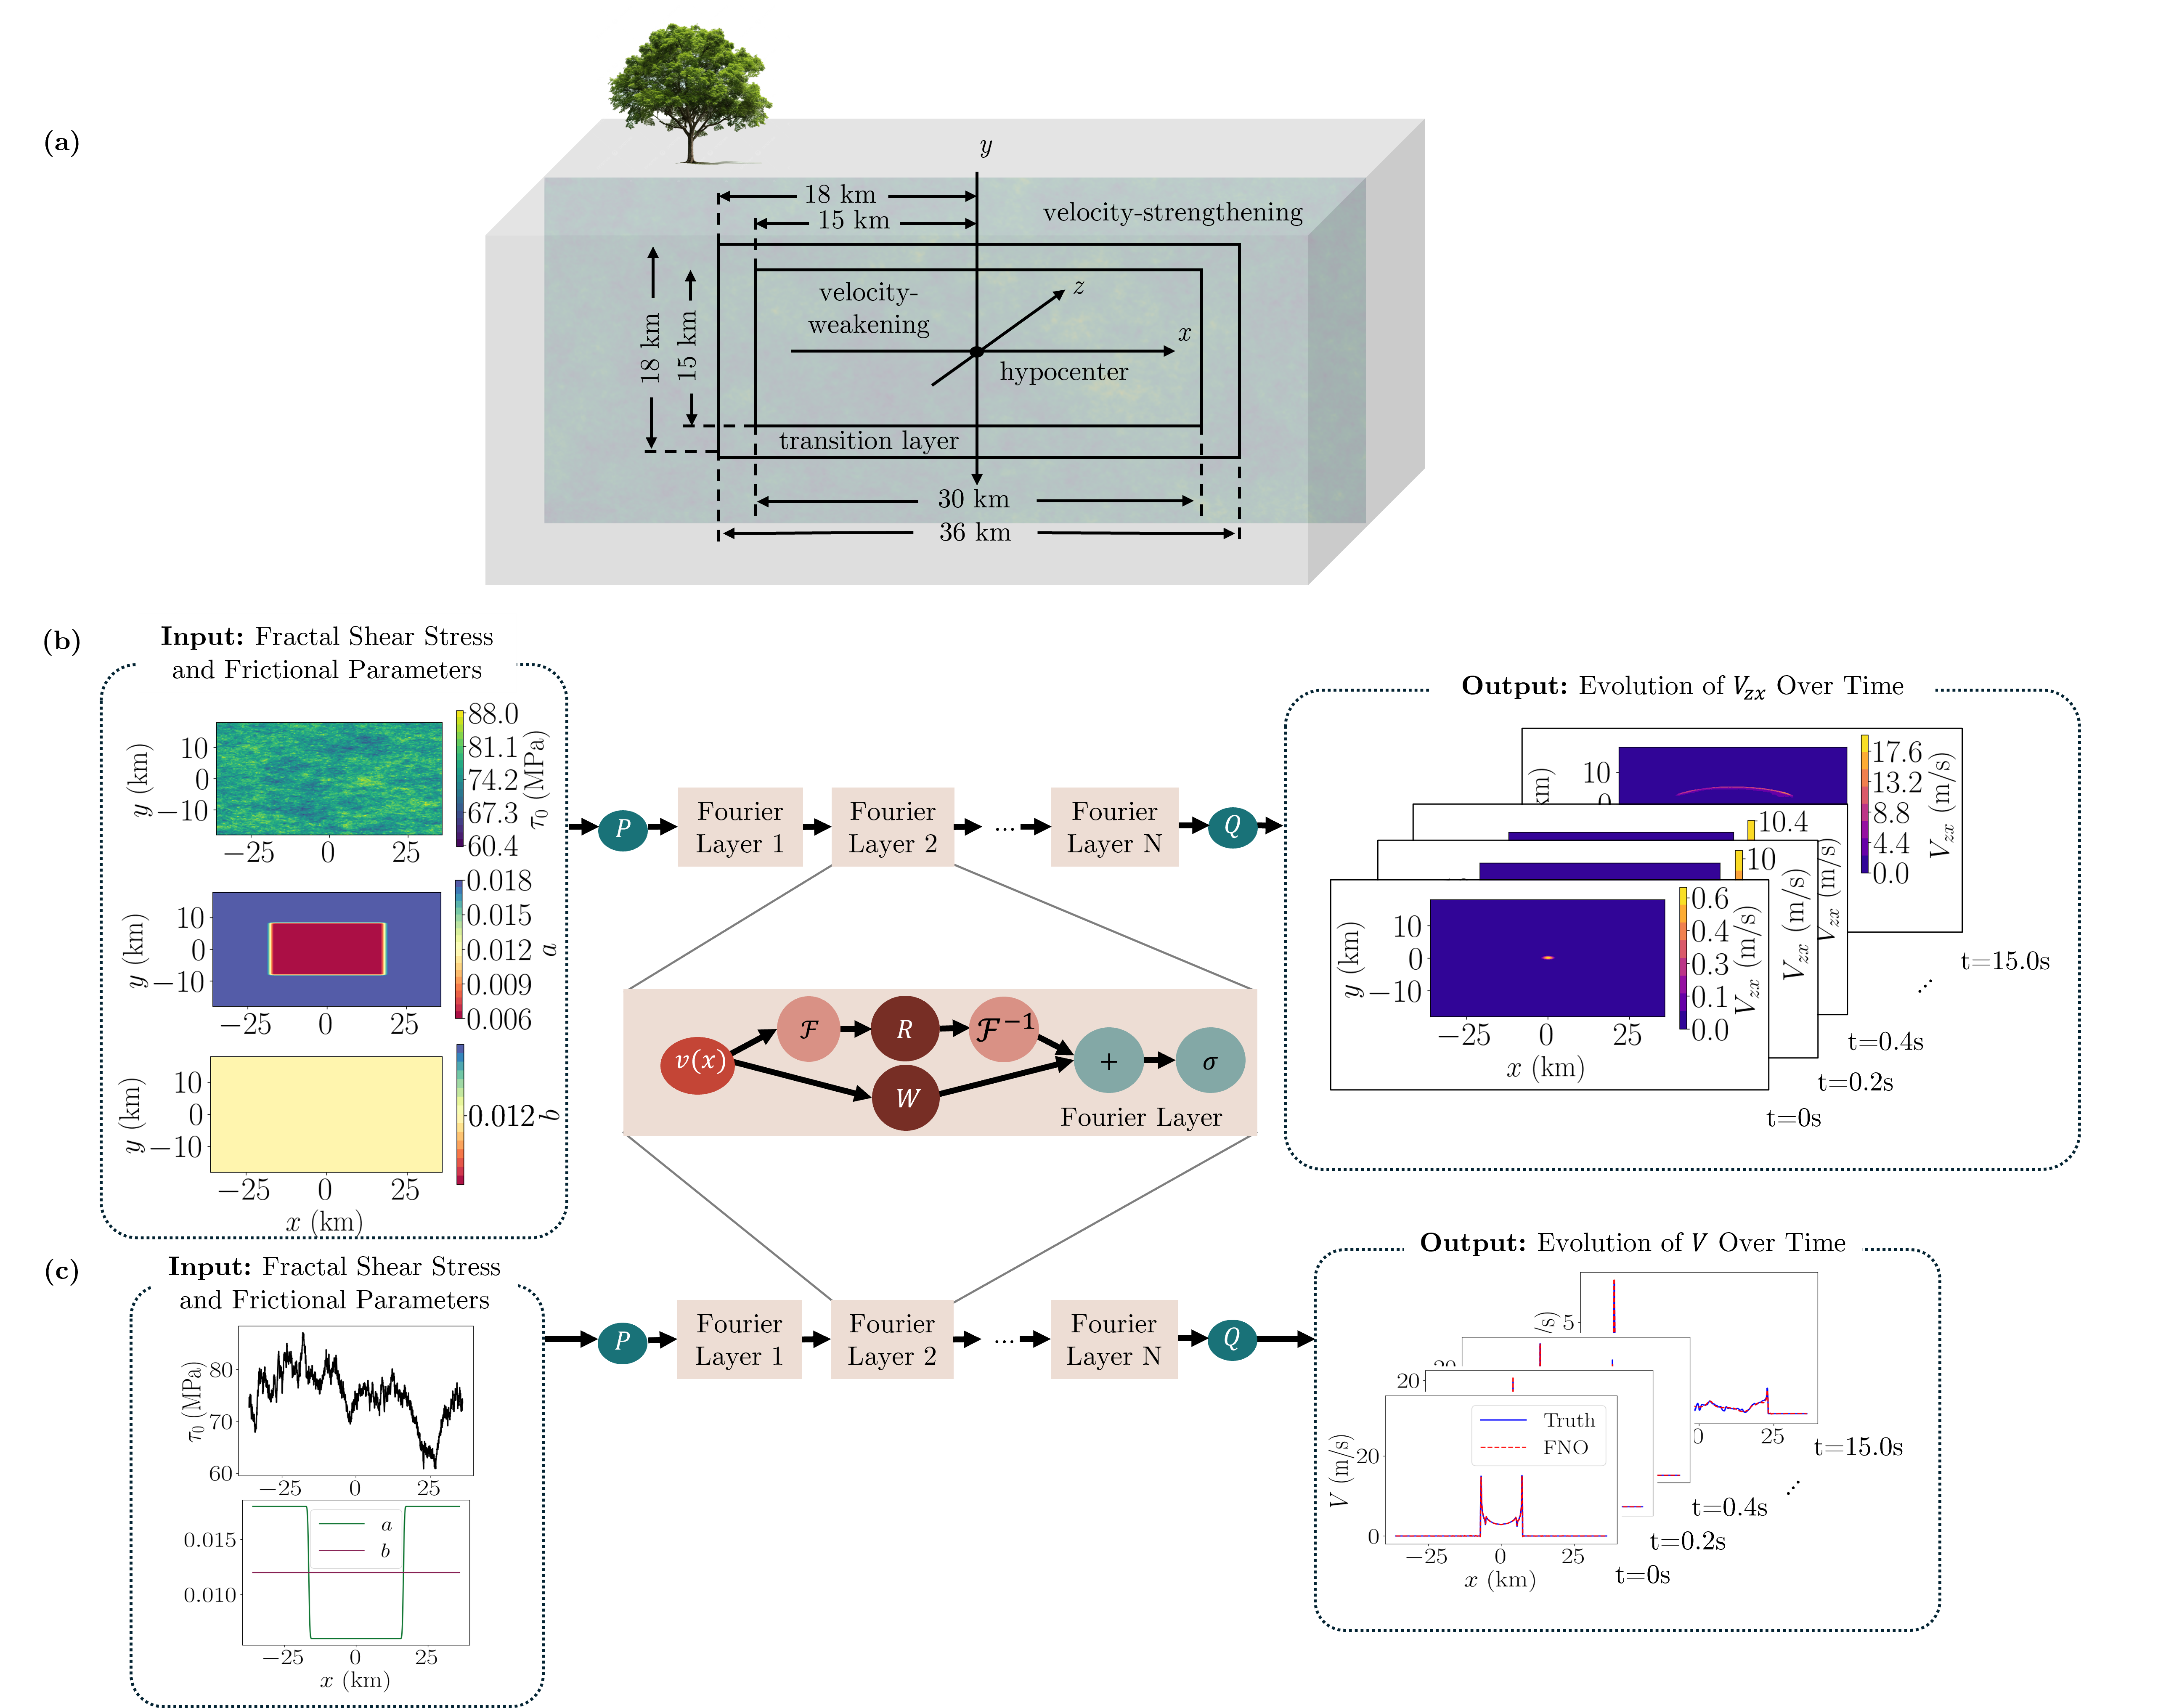
\includegraphics[width=1.0\linewidth]{FNO_framework6.png}
%DIFDELCMD < %%%
\DIFdelendFL \DIFaddbeginFL 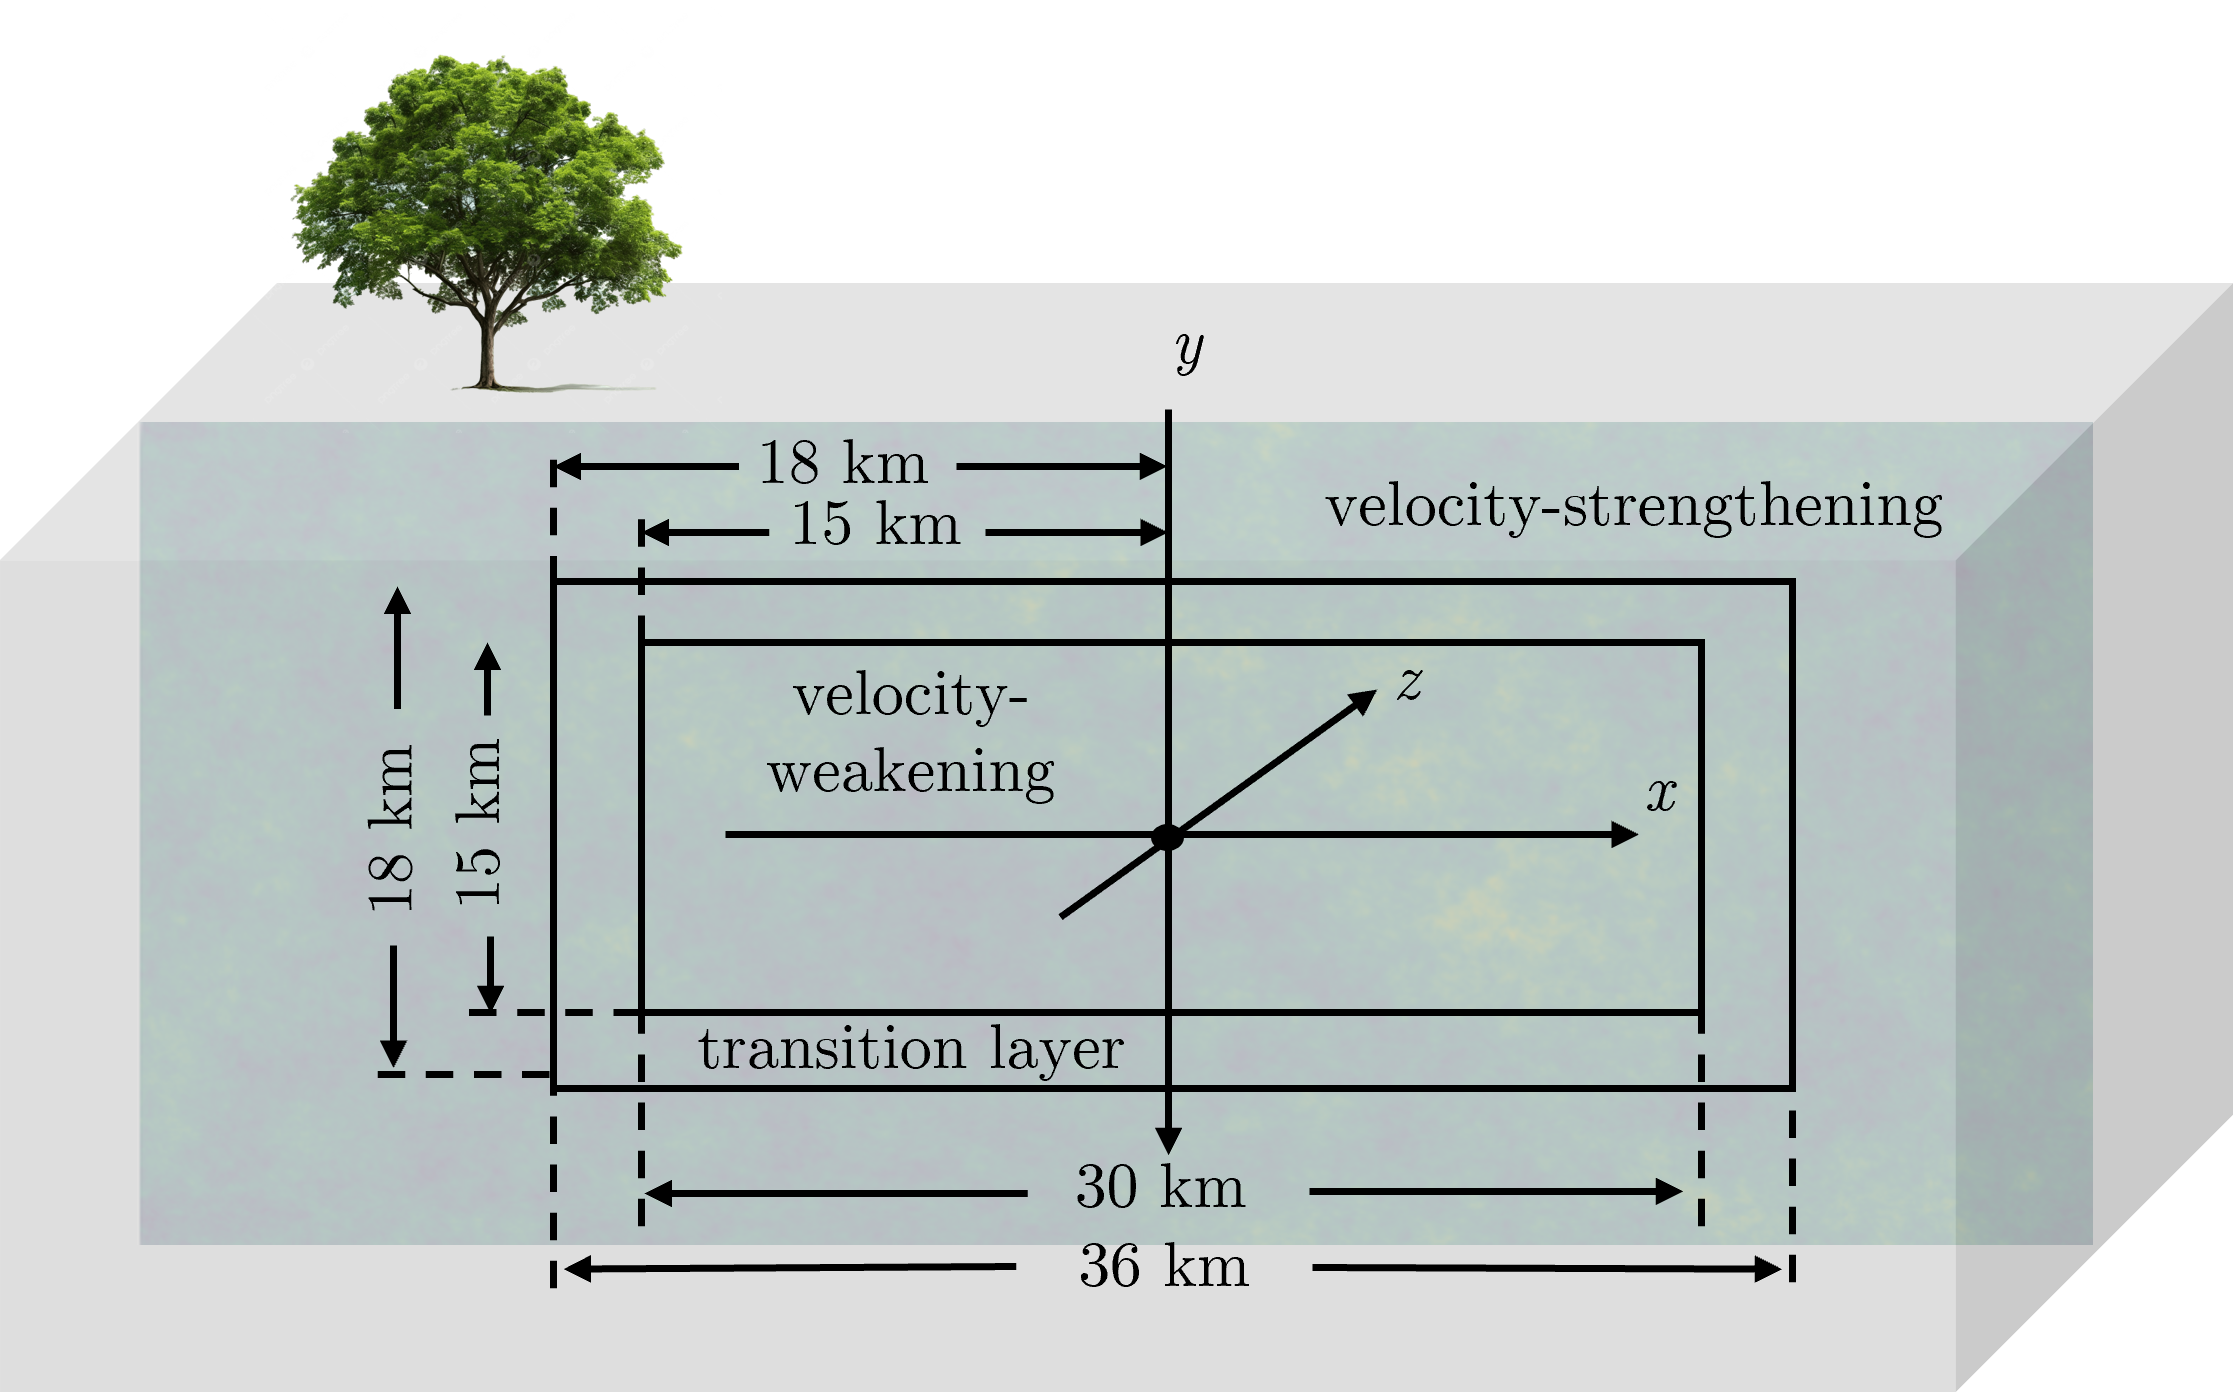
\includegraphics[width=0.5\linewidth]{fault_model.png}
\DIFaddendFL \caption{\DIFdelbeginFL %DIFDELCMD < \label{fig:schematic_FNO}%%%
\DIFdelendFL \DIFaddbeginFL \label{fig:schematic_fault}\DIFaddendFL Schematic \DIFdelbeginFL \DIFdelFL{diagram of the proposed FNO framework. (a) Schematic }\DIFdelendFL illustration of the \DIFaddbeginFL \DIFaddFL{3D }\DIFaddendFL fault model, showing the central VW regime surrounded by the VS regime \DIFdelbeginFL \DIFdelFL{, with the hypocenter at the center. (b) FNO framework for }\DIFdelendFL \DIFaddbeginFL \DIFaddFL{separated by }\DIFaddendFL a \DIFdelbeginFL \DIFdelFL{2D fault plane embedded in a 3D bulk}\DIFdelendFL \DIFaddbeginFL \DIFaddFL{transition layer}\DIFaddendFL . \DIFdelbeginFL \DIFdelFL{(c) FNO framework for a 1D fault embedded in a 2D plane. }\DIFdelendFL The \DIFdelbeginFL \DIFdelFL{inputs include the distribution of initial }\DIFdelendFL shear stress \DIFaddbeginFL \DIFaddFL{follows a fractal distribution, }\DIFaddendFL and \DIFdelbeginFL \DIFdelFL{frictional parameters}\DIFdelendFL \DIFaddbeginFL \DIFaddFL{the hypocenter is varied within the VW region}\DIFaddendFL .
\DIFdelbeginFL \DIFdelFL{The outputs are snapshots of slip rate over time.
}\DIFdelendFL }
\end{figure}

We introduce variations into the initial shear stress field (\(\tau_{0}\)) to capture spatial stress heterogeneity, which studies suggest follows a fractal-like distribution consistent with the roughness of fault surfaces \cite{andrews1980stochastic,renard2017scaling}. Moreover, models incorporating fractal distributions align with key seismological patterns, such as the Gutenberg-Richter law \cite{hirata1989correlation}. We generate a fractal shear stress field with a specified fractal dimension \(D\), mean, and standard deviation. The frequency-domain representation is constructed using a power-law scaling:

\begin{equation}
P(k) \propto \frac{1}{k^{2.5-D}},
\label{eq:amp}
\end{equation}

where \(k\) is the normalized wavenumber. This scaling yields larger amplitudes at low wavenumbers and smaller amplitudes at high wavenumbers.

We assign a random phase \( \phi \) to each frequency component. The phase is drawn from a uniform distribution \( \phi \sim \mathcal{U}(0, 2\pi) \). The complex frequency-domain representation is constructed as:

\begin{equation}
\label{eqn:domian_freq}
\text{Spectrum} = P(k) \cdot \left[ \cos(\phi) + i \sin(\phi) \right],
\end{equation}

After constructing the spectrum, we apply an inverse FFT to transform the data back into the spatial domain. The resulting real-valued shear stress field is normalized to ensure it matches the target statistical properties, including the specified mean and standard deviation:

\begin{equation}
\label{eqn:normalized_fractal}
S'(x) = \frac{S(x) - \mu}{\sigma} \cdot \sigma' + \mu',
\end{equation}

where $\mu$ and $\sigma$ are the mean and standard deviation of the raw field $S(x)$, and $\mu'$ and $\sigma'$ are the mean and standard deviation of the scaled field $S'(x)$, respectively.

The \DIFdelbegin \DIFdel{fault's }\DIFdelend \DIFaddbegin \DIFadd{dynamic rupture dataset is generated using the Spectral Boundary Integral (SBI) method, which is currently the fastest available solver for simulating rupture propagation along a planar fault in a homogeneous medium \mbox{%DIFAUXCMD
\cite{geubelle1995spectral}}\hskip0pt%DIFAUXCMD
. This method involves solving the coupled equations governing traction and displacement continuity along the fault surface. As a result, it eliminates the need to solve the governing equations throughout the entire domain. According to \mbox{%DIFAUXCMD
\cite{geubelle1995spectral}}\hskip0pt%DIFAUXCMD
, the response of the governing equations \ref{eq:momentum_balance}–\ref{eq:fault_bc} is given by
}

\begin{equation}
\DIFadd{\label{eqn:sbi}
\tau_i(x_1, x_3, t) = \tau_i^0 - \eta^{\pm}_{ij} \, \dot{u}^{\pm}_j(x_1, x_3, t) + f^{\pm}_i(x_1, x_3, t),
}\end{equation}

\DIFadd{where \(\tau_{i}\) is the traction at the fault's surface on the half-space lying in the \(x_{1}\)–\(x_{3}\) plane. \(\tau_i^0\) denotes the far-field traction. \(\dot{u}_i\) denotes the particle velocity, \(\eta_{ij}\) is the radiation damping coefficient matrix, and \(f_i\) represents an integral term of the deformation history, computed via time convolution in the spectral domain.
}

\DIFadd{In SBI simulations, the fault's }\DIFaddend initial slip rate is prescribed as the constant $V_{ini}=10^{-12}$ m/s. To satisfy the friction law, the initial state variable is computed for each spatial location, incorporating the spatial variability of the parameter $a$ and the imposed fractal shear stress distribution. The rupture is started by artificially overstressing a fault segment. \DIFaddbegin \DIFadd{The hypocenter location varies across realizations but remains within the VW regime. }\DIFaddend Details of this nucleation procedure are provided in \DIFdelbegin \DIFdel{Appendix \ref{sec:appendix_a}. }\DIFdelend \DIFaddbegin \DIFadd{\ref{sec:appendix_a}. We adopt UGUCA code \mbox{%DIFAUXCMD
\cite{kammer2021uguca} }\hskip0pt%DIFAUXCMD
to generate the dynamic rupture dataset.
}\DIFaddend 



\begin{table}[ht!]
\caption{\label{table:2D_parameters}\DIFdelbeginFL \DIFdelFL{Parameters for the fault }\DIFdelendFL \DIFaddbeginFL \DIFaddFL{Fault }\DIFaddendFL model \DIFaddbeginFL \DIFaddFL{parameters in the Spectral Boundary Integral (SBI) framework}\DIFaddendFL }
\centering
\begin{tabular}{@{}lll@{}}
\toprule
\textbf{Medium Parameter}       & \textbf{Symbol} & \textbf{Value} \\ \midrule
Shear wave speed (km/s)         & $c_s$           & 3.464            \\
Pressure wave speed (km/s)      & $c_p$           & 6            \\
Density (kg/m\(^3\))            & $\rho$          & 2670         \\\midrule
\textbf{Fault Parameters}       &                 &                \\ \midrule
Reference coefficient of friction & $f^*$          & 0.6            \\
Characteristic slip (m)         & $D_{RS}$             & 0.02             \\
Reference slip velocity (m/s)   & $V^*$           & $10^{-6}$      \\
Length of VW patch in $x$ direction (km)          & $2W$        & 30             \\
Width of VW patch in $y$ direction (km)          & $W$        & 15             \\
Length of transition (km)        & $w$     & 3             \\
Length of the fault in $x$ direction (km)         & $L_{fx}$           & 72             \\
Width of the fault in $y$ direction (km)         & $L_{fy}$           & 36             \\
Evolution effect parameter      & $b$             & 0.012          \\
Steady state velocity dependence in VW patch & $a_{VW} - b$ & varies \\
Steady state velocity dependence in VS patch & $a_{VS} - b$ & varies   \\ 
Initial velocity (m/s)          & $V_{ini}$     & $10^{-12}$ \\
Initial normal stress (MPa)     & $\sigma_{ini}$ & 120 \\
Target mean of fractal shear stress (MPa) & $\mu'$ & 75 \\
Target standard deviation of fractal shear stress (MPa) & $\sigma'$ & 5 \\ \midrule
\textbf{Nucleation Parameters}  &                 &                \\ \midrule
Nucleation radius (km)             & $R$      & 3           \\
Maximum nucleation amplitude (MPa) & $\Delta\tau_{0}$        & 25            \\
Final nucleation time (s) & $T$        & 1            \\
\bottomrule
\end{tabular}
\end{table}

\DIFaddbegin \subsection{\DIFadd{Fourier Neural Operators}}
\label{sec:fno}

\DIFadd{The Fourier Neural Operator (FNO) is a learning-based operator designed to map between infinite-dimensional spaces using input-output pairs, $\{a_j, u_j\}_{j=1}^{N}$. FNO replaces the kernel integral operator in traditional neural operators with a convolution operator defined in Fourier space. Subsequently, an inverse Fourier transform is applied, along with a linear transformation. The resulting values are then passed through an activation function, which is applied to the sum of the transformed features. Mathematically, the neural operator follows an iterative update process, $v_0 \rightarrow v_1 \rightarrow v_2 \rightarrow \dots \rightarrow v_T$, where the update from $v_0$ to $v_M$ and the output $u(x)$ are defined as follows:
}

\begin{equation}
\DIFadd{\label{eqn:fno}
\begin{aligned}
    v_{0}(x) &= P(a(x)) \\
    v_{m+1}(x) &= \sigma\left(W_{m} v_{m}(x) + \int k(x,y)_{m} v_{m}(y)\,dy \right), \quad m=0,\dots,M-1 \\
    u(x) &= Q(v_{M}(x))
\end{aligned}
}\end{equation}

\DIFadd{where $P$ is a pointwise lifting operator parameterized with a neural network that projects the point values of input function $a(x)$ to a higher dimension. $W_m$ is a linear transformation applied to $v_m(x)$ to account for non-periodic boundary conditions. $\int k(x,y) v_m(y),dy$ represents a kernel integral operator. $Q$ is a pointwise projection operator parameterized with a neural network that maps back to the target dimension. $\sigma$ is a nonlinear activation function.
}

\DIFadd{In FNO, we replace the kernel integral operator with a convolution operator using the fast Fourier transform. Thus, we can rewrite the kernel integral operator as follows:
}

\begin{equation}
\DIFadd{\label{eqn:kernel}
    \int k(x,y)_{m} v_{m}(y)\,dy  = \mathcal{F}^{-1}(\mathcal{F}(k_m) \cdot \mathcal{F}(v_m))
}\end{equation}

\DIFadd{where $\mathcal{F}$ and $\mathcal{F}^{-1}$ are the Fourier transform and its inverse, respectively. Using the Fourier transform enhances computational efficiency, allows the model to handle global dependencies, and enables resolution invariance, meaning the model can generalize across different spatial and temporal resolutions without requiring retraining. Specifically, when the input function is provided in regular grids, the Fourier transformer is carried using fast Fourier transform, a celebrated and fast algorithm for Fourier analysis. It also leads to better generalization across grids, reduces computational costs for high-dimensional problems, and improves the model's ability to handle complex, nonlinear dynamics. We refer the reader to \mbox{%DIFAUXCMD
\cite{li2020fourier} }\hskip0pt%DIFAUXCMD
for a discussion of this architecture and related features.
}

\DIFadd{Here, the FNO is designed to take as inputs the initial shear stress, the slip rate \(V\) for the 2D case or its component \(V_{zx}\) in 3D, frictional parameters, and the nucleation stress perturbation. The model outputs the evolution of the slip rate \(V\) in 2D or \(V_{zx}\) in 3D, as illustrated in Figure~\ref{fig:schematic_FNO}. We use this framework to allow for variations in (1) the initial fractal distribution of shear stress, (2) the initial stage of the rupture realization (i.e., the input can be provided at different time point in the simulation), (3) the values of frictional parameters \(a\) and \(b\), and (4) the location of nucleation sites. This setup captures the variability and uncertainty inherent in natural faults, where initial stress conditions, frictional properties, and nucleation behavior are often poorly constrained or spatially heterogeneous.
}

\begin{figure}
\centering
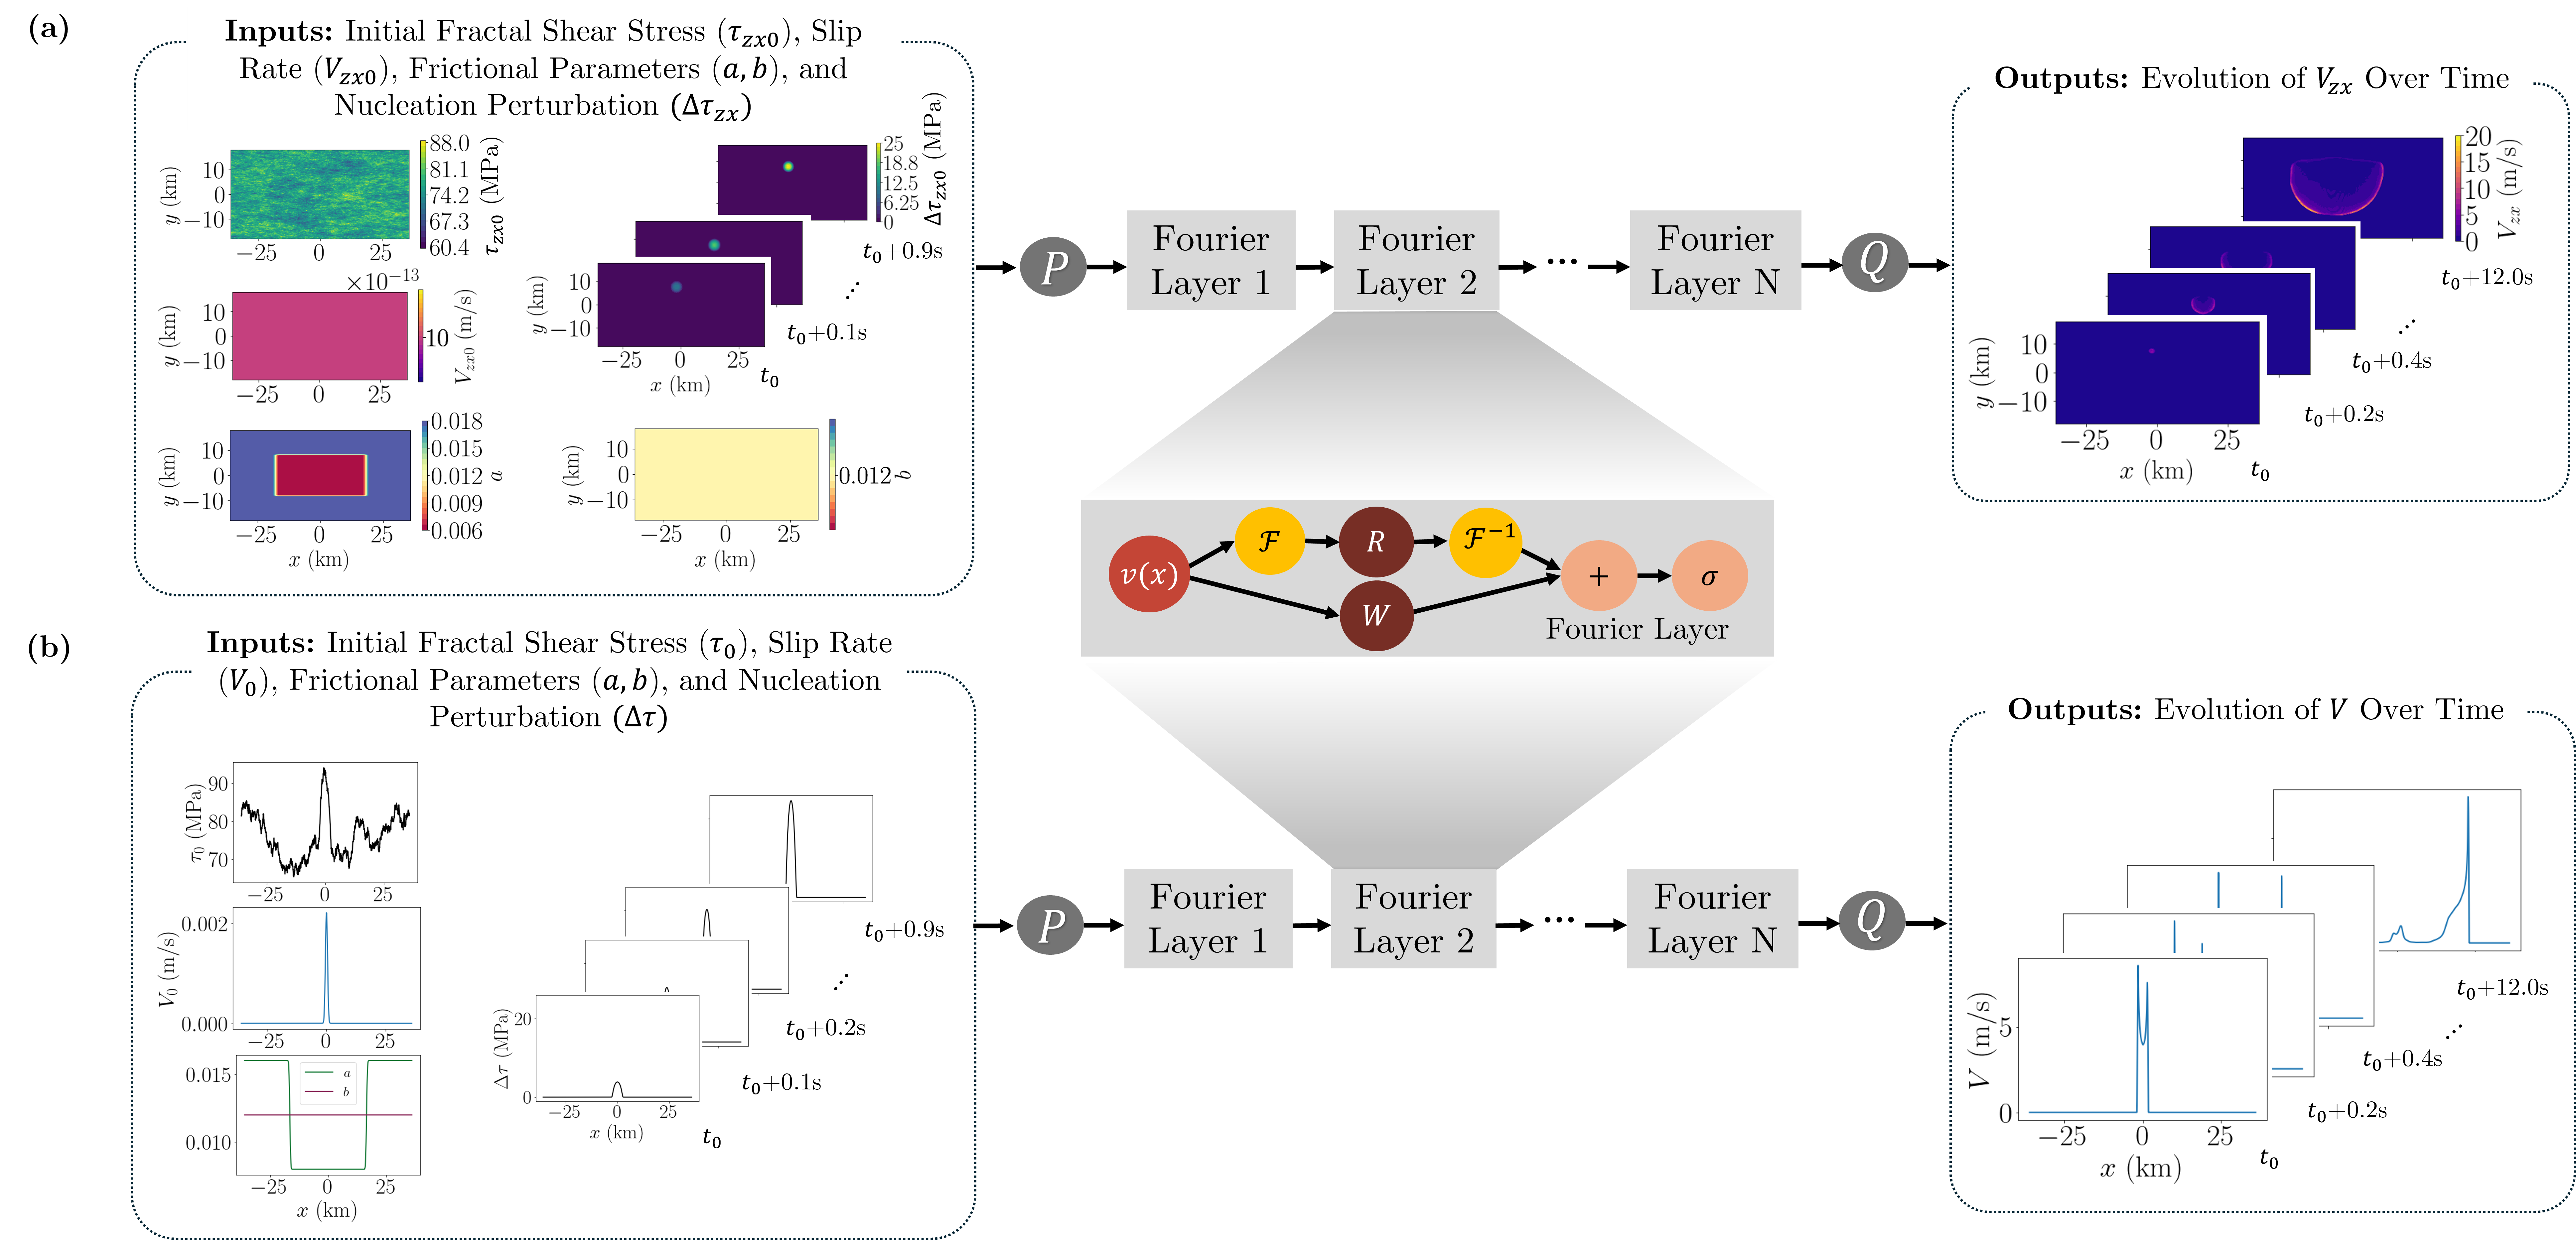
\includegraphics[width=1.0\linewidth]{fno_framework.png}
\caption{\label{fig:schematic_FNO}\DIFaddFL{Schematic diagram of the proposed FNO framework. (a) FNO framework for a 2D fault plane embedded in a 3D bulk. (c) FNO framework for a 1D fault embedded in a 2D plane. The inputs include the distribution of initial shear stress, slip rate, frictional parameters, and stress perturbation of nucleation. The outputs are snapshots of slip rate over time.
}}
\end{figure}

\DIFaddend \subsection{Evaluating Model Predictions}
\label{sec:eval}

The accuracy of predictions is assessed using a measure of the difference between the ground truth and the predicted slip rate over time. We present two error metrics: the relative \(L_2\) error and the normalized root mean squared error (NRMSE). During the training and testing stages, the loss function is calculated using the relative \(L_2\) error:

\begin{equation}
\label{eqn:rel_l2}
\text{Relative } L_2 \text{ error} = \frac{\| V_{\text{pred}}(\mathbf{x}, t) - V_{\text{true}}(\mathbf{x}, t) \|_2}{\| V_{\text{true}}(\mathbf{x}, t) \|_2}
\end{equation}

where \(V_{\text{pred}}(\mathbf{x}, t)\) is the predicted slip rate at location \(\mathbf{x}\) and time \(t\), and \(V_{\text{true}}(\mathbf{x}, t)\) is the corresponding true value. However, this metric can be misleading sometimes because the slip rate is close to zero at some points. As a result, the metric can be disproportionately influenced. 

Moreover, shifts in space and time are inherent in the dynamic rupture problem \cite{barall2015metrics}. These shifts introduce bias into the relative \(L_2\) error calculation, especially when the shifted prediction is compared to a small ground truth value. These biases will be discussed in each of the results sections. To address this issue, we introduce another metric, NRMSE:

\begin{equation}
\label{eqn:NRMSE}
\text{NRMSE} = \frac{\sqrt{\frac{1}{M N} \sum_{i=1}^{M} \sum_{j=1}^{N} \left( V_{\text{pred}, j}^{(i)} - V_{\text{true}, j}^{(i)} \right)^2 }}{V_{\max} - V_{\min}}
\end{equation}

where \(M\) is the total number of time steps, \(N\) is the total number of spatial points, \(V_{\text{pred}, j}^{(i)}\) is the predicted value at spatial point \(j\) and time step \(i\), and \(V_{\text{true}, j}^{(i)}\) is the corresponding true value obtained from the numerical simulations. \(V_{\max}\) and \(V_{\min}\) are the maximum and minimum values of \(V_{\text{true}}\) over the entire space-time domain. NRMSE compares the error with the observed range of the ground truth. As such, the predictions will not be disproportionately influenced by small ground truth values.

\section{Data Configuration}
\label{sec:data}

 \DIFdelbegin \DIFdel{The dynamic rupture dataset is generated using the Spectral Boundary Integral (SBI ) method, which is currently the fastest available solver for rupture propagation on a planar fault in a homogeneous medium \mbox{%DIFAUXCMD
\cite{geubelle1995spectral,kammer2021uguca}}\hskip0pt%DIFAUXCMD
.  The }\DIFdelend \DIFaddbegin \DIFadd{In the SBI solver, the }\DIFaddend key parameters used in the model are summarized in Tables \ref{table:2D_parameters} and \DIFdelbegin \DIFdel{\ref{table:dataset_description}}\DIFdelend \DIFaddbegin \DIFadd{\ref{tab:dataset_summary}}\DIFaddend . The fractal dimensions are chosen to represent natural faults, with \( D \) varying between 1.2 and 1.6 \cite{renard2017scaling}. The rate-and-state frictional parameters fall within the observed range from laboratory experiments \DIFdelbegin \DIFdel{\mbox{%DIFAUXCMD
\cite{ikari2011relation}}\hskip0pt%DIFAUXCMD
}\DIFdelend \DIFaddbegin \DIFadd{\mbox{%DIFAUXCMD
\cite{ikari2011relation, barbot2022rate}}\hskip0pt%DIFAUXCMD
}\DIFaddend . The dataset is obtained by solving the dynamic rupture problem over the time interval \( [0,15] \) s. 

Two datasets are generated, corresponding to 2D and 3D dynamic rupture simulations. The 3D simulation treats the fault as a 2D plane embedded in a 3D bulk, which is trained using FNO-2D, as shown in Figure \ref{fig:schematic_FNO}\DIFdelbegin \DIFdel{b}\DIFdelend \DIFaddbegin \DIFadd{a}\DIFaddend . It employs a 2D Fourier Transform to capture spatial correlations in both dimensions. The 2D simulation treats the fault as a 1D cross-section along the hypocenter in the \( x \)-axis. This dataset is trained using a separate FNO-1D, as shown in Figure \ref{fig:schematic_FNO}\DIFdelbegin \DIFdel{c}\DIFdelend \DIFaddbegin \DIFadd{b}\DIFaddend . It applies a 1D Fourier Transform to extract frequency features and efficiently learn spatial dependencies. 

For the initial shear stress distribution, expressed in Equation \ref{eq:amp}, the normalized wave number \( k_i \) for the 1D fault is defined as:

\begin{equation}
\label{eqn:k_2D}
k_i = \frac{i}{n_x}
\end{equation}

where \( n_x \) is the total number of spatial points. We set \( k_0 = 1 \) for \( i = 0 \) to avoid division by zero. This choice is arbitrary as it only affects the mean value of the stress distribution which gets overridden later by matching the target mean value.

For the 2D fault, each grid point \( (i,j) \) in Fourier space corresponds to a wave number pair \( (k_x, k_y) \), defined as:

\begin{equation}
\label{eqn:k_3D}
k_x = \frac{i}{n_x}, \quad k_y = \frac{j}{n_y}, \quad
k = \sqrt{k_x^2 + k_y^2}
\end{equation}

where \( n_x \) and \( n_y \) are the total number of points in the \( x \) and \( y \) directions, respectively.


\subsection{2D Dynamic Rupture Dataset}
\label{sec:2d}

In the 2D dataset, the fault is represented as a one-dimensional line embedded in a \DIFdelbegin \DIFdel{two-dimensional elastic bulk}\DIFdelend \DIFaddbegin \DIFadd{2D elastic bulk, }\DIFaddend assuming plane strain conditions. A total of \DIFdelbegin \DIFdel{4,000 }\DIFdelend \DIFaddbegin \DIFadd{8,200 }\DIFaddend realizations are generated, with \DIFdelbegin \DIFdel{1,000 realizations for each parameter set }\DIFdelend \DIFaddbegin \DIFadd{parameters }\DIFaddend listed in Table~\DIFdelbegin \DIFdel{\ref{table:dataset_description}. Of these, 3,600 realizations are allocated for training, while the remaining 400 realizationsare reserved for }\DIFdelend \DIFaddbegin \DIFadd{\ref{tab:dataset_summary}. Among these, 4,000 realizations have the hypocenter at the center of the fault, 2,100 have hypocenters located at the point of maximum shear stress in the VW region, and the remaining 2,100 have randomly located hypocenters drawn from a uniform distribution along the fault. 
}

\DIFadd{Each realization is processed to create four different starting points based on a slip rate threshold, \(V_\text{th}\). We define this threshold as the time step when the maximum slip rate in the domain first exceeds \(V_\text{th}\). From that point, we extract the input features: initial shear stress, slip rate, and nucleation perturbation. The frictional parameters are kept unchanged across all starting points. We use four threshold values: \(V_\text{th} \in \{0, 10^{-4}, 10^{-3}, 10^{-2}\}\). These thresholds are typically used to define the onset of seismic events in multi cycles simulations. This approach results in four sets of data for each of the original 8,200 realizations, giving a total of 32,800 data samples. Of these, 28,700 are used for training and 4,100 for }\DIFaddend testing.

The FNO is trained to approximate the mapping from the initial shear stress \DIFdelbegin \DIFdel{and }\DIFdelend \DIFaddbegin \DIFadd{\(\tau_0\), slip rate \(V_0\), }\DIFaddend frictional parameters \( a \) and \( b \)\DIFaddbegin \DIFadd{, and stress perturbation \(\Delta\tau\) }\DIFaddend to the sequence of slip rates over the time interval of interest. The input data is structured as a tensor of dimensions \( (N, X, C_{\text{in}}) \), while the output data has dimensions \( (N, X, C_{\text{out}}) \), where \( N \) denotes the number of realizations, \( X \) represents the number of spatial discretization points, \( C_{\text{in}} \) and \( C_{\text{out}} \) correspond to the number of input and output channels, respectively.

The spatial discretization consists of 2,880 points, i.e., \DIFdelbegin \DIFdel{\( X = 2,880 \), which corresponds to the discretization of }\DIFdelend \DIFaddbegin \DIFadd{\( X = 2{,}880 \), consistent with the resolution used in }\DIFaddend the SBI solver. The input channels \DIFdelbegin \DIFdel{comprise }\DIFdelend \DIFaddbegin \DIFadd{include }\DIFaddend the spatial distributions of \DIFaddbegin \DIFadd{the }\DIFaddend initial shear stress \DIFdelbegin \DIFdel{, parameter \( a \), and parameter \( b \), resulting in \( C_{\text{in}} = 3 \). }\DIFdelend \DIFaddbegin \DIFadd{\(\tau_0\) and slip rate at \(t_0\), frictional parameters \(a\) and \(b\), and ten time steps of the nucleation stress perturbation \(\Delta \tau\), sampled at 0.1~s intervals starting from the time \(t_0\), when the slip rate first exceeds the threshold \(V_\text{th}\). These ten perturbation snapshots correspond to \(t = t_0, t_0 + 0.1~\text{s}, \ldots, t_0 + 0.9~\text{s}\), contributing ten additional input channels. In total, this yields \(C_{\text{in}} = 14\). This potentially opens up the possibility of using different nucleation over-stress distribution.
}\DIFaddend 

We solve the \DIFdelbegin \DIFdel{system of equations using SBI }\DIFdelend \DIFaddbegin \DIFadd{governing equations using the SBI solver }\DIFaddend with a time step \DIFdelbegin \DIFdel{\(\Delta t\) of 0.001 s to satisfy }\DIFdelend \DIFaddbegin \DIFadd{of \(\Delta t = 0.001~\text{s}\), which satisfies }\DIFaddend the Courant–Friedrichs–Lewy (CFL) condition, \DIFdelbegin \DIFdel{\(\Delta t \leq f \Delta x/c_p\) with }\DIFdelend \DIFaddbegin \DIFadd{\(\Delta t \leq f \Delta x / c_p\), where }\DIFaddend \(f\) is \DIFdelbegin \DIFdel{of order 1. Herewe take \(f\) equal to 0.25}\DIFdelend \DIFaddbegin \DIFadd{a constant of order one. Here, we choose \(f = 0.25\)}\DIFaddend . Since FNOs are independent of \DIFaddbegin \DIFadd{the numerical }\DIFaddend discretization, we \DIFdelbegin \DIFdel{can use }\DIFdelend \DIFaddbegin \DIFadd{adopt }\DIFaddend a coarser time step \DIFdelbegin \DIFdel{in FNO because we aim }\DIFdelend \DIFaddbegin \DIFadd{of 0.2~s in the FNO model. The FNO is trained }\DIFaddend to perform a single-shot prediction \DIFdelbegin \DIFdel{up to 15 s, and a time step of 0.001 s poses significant memory challenges. As such, the output channels represent snapshots of the slip rate at discrete }\DIFdelend \DIFaddbegin \DIFadd{of 60 }\DIFaddend time steps of \DIFdelbegin \DIFdel{0.2 s, spanning the duration from \( t = 0 \) s to \( t = 15 \) s, yielding 76 time steps and thus \( C_{\text{out}} = 76 \)}\DIFdelend \DIFaddbegin \DIFadd{slip rate, starting from time \(t_0\), resulting in \(C_{\text{out}} = 60\)}\DIFaddend .


Before training, the dataset is normalized, scaling each feature in both the input and output to the range \([0,1]\). After training, the original physical scale is restored using an inverse transformation. This normalization enhances numerical stability and facilitates efficient training of the FNO model \cite{cuomo2022scientific}.

\DIFdelbegin %DIFDELCMD < \begin{table}[ht!]
%DIFDELCMD < %%%
%DIFDELCMD < \caption{%
{%DIFAUXCMD
%DIFDELCMD < \label{table:dataset_description}%%%
\DIFdelFL{Fractal dimensions and variation of frictional parameter \(a\) and \(b\) for 2D and 3D dynamic rupture dataset}}
%DIFAUXCMD
\DIFdelendFL \DIFaddbeginFL \begin{table}[htbp]
\centering
\caption{\DIFaddFL{Fractal dimensions and variation of frictional parameter \(a\) and \(b\) for 2D and 3D dynamic rupture dataset}}
\label{tab:dataset_summary}
\begin{tabular}{llll}
\toprule
\DIFaddbeginFL $D$ & $b$ & $a_0$ & $\Delta a_0$ \\
\midrule
1.2, 1.5, 1.6 & 0.012, 0.014 & 0.009 & 0.006 \\
1.2, 1.5, 1.6 & 0.012, 0.014 & 0.008 & 0.008 \\
1.2, 1.5, 1.6 & 0.012, 0.014 & 0.007 & 0.010 \\
1.2, 1.5, 1.6 & 0.012, 0.014 & 0.006 & 0.012 \\
1.2, 1.5, 1.6 & 0.012, 0.014 & 0.0085 & 0.007 \\
1.2, 1.5, 1.6 & 0.012, 0.014 & 0.0075 & 0.009 \\
1.2, 1.5, 1.6 & 0.012, 0.014 & 0.0065 & 0.011 \\
\bottomrule
\end{tabular}
\end{table}
\DIFaddendFL

\subsection{3D Dynamic Rupture Dataset}
\label{sec:3d}

In the 3D dataset, the fault is modeled as a \DIFdelbegin \DIFdel{two-dimensional }\DIFdelend \DIFaddbegin \DIFadd{2D }\DIFaddend plane embedded in a \DIFdelbegin \DIFdel{three-dimensional }\DIFdelend \DIFaddbegin \DIFadd{3D }\DIFaddend elastic bulk. \DIFdelbegin \DIFdel{A total of 4,000 realizations are generated, with 3,600 realizations used for training and 400 realizations for testing. }\DIFdelend The variations in fractal dimension and frictional parameters \( a \) and \( b \) are listed in Table \DIFdelbegin \DIFdel{\ref{table:dataset_description}, with each parameter set containing 1,000 realizations}\DIFdelend \DIFaddbegin \DIFadd{\ref{tab:dataset_summary}}\DIFaddend . Examples of fractal initial shear stress distributions generated using different fractal dimensions are illustrated in Figure \ref{fig:3D_contour}. 

\DIFaddbegin \DIFadd{Similar to the 2D case, 8,200 realizations are generated: 4,000 with the hypocenter at the fault center, 2,100 at the location of maximum shear stress in the VW region, and 2,100 with uniformly random hypocenter locations. Each realization is processed in the same manner as the 2D case to produce four distinct initial conditions based on the slip rate threshold \(V_\text{th} \in \{0, 10^{-4}, 10^{-3}, 10^{-2}\}\). This results in 32,800 data samples. From these, 28,700 are used for training and 4,100 for testing.
}

\DIFaddend \begin{figure}
\centering
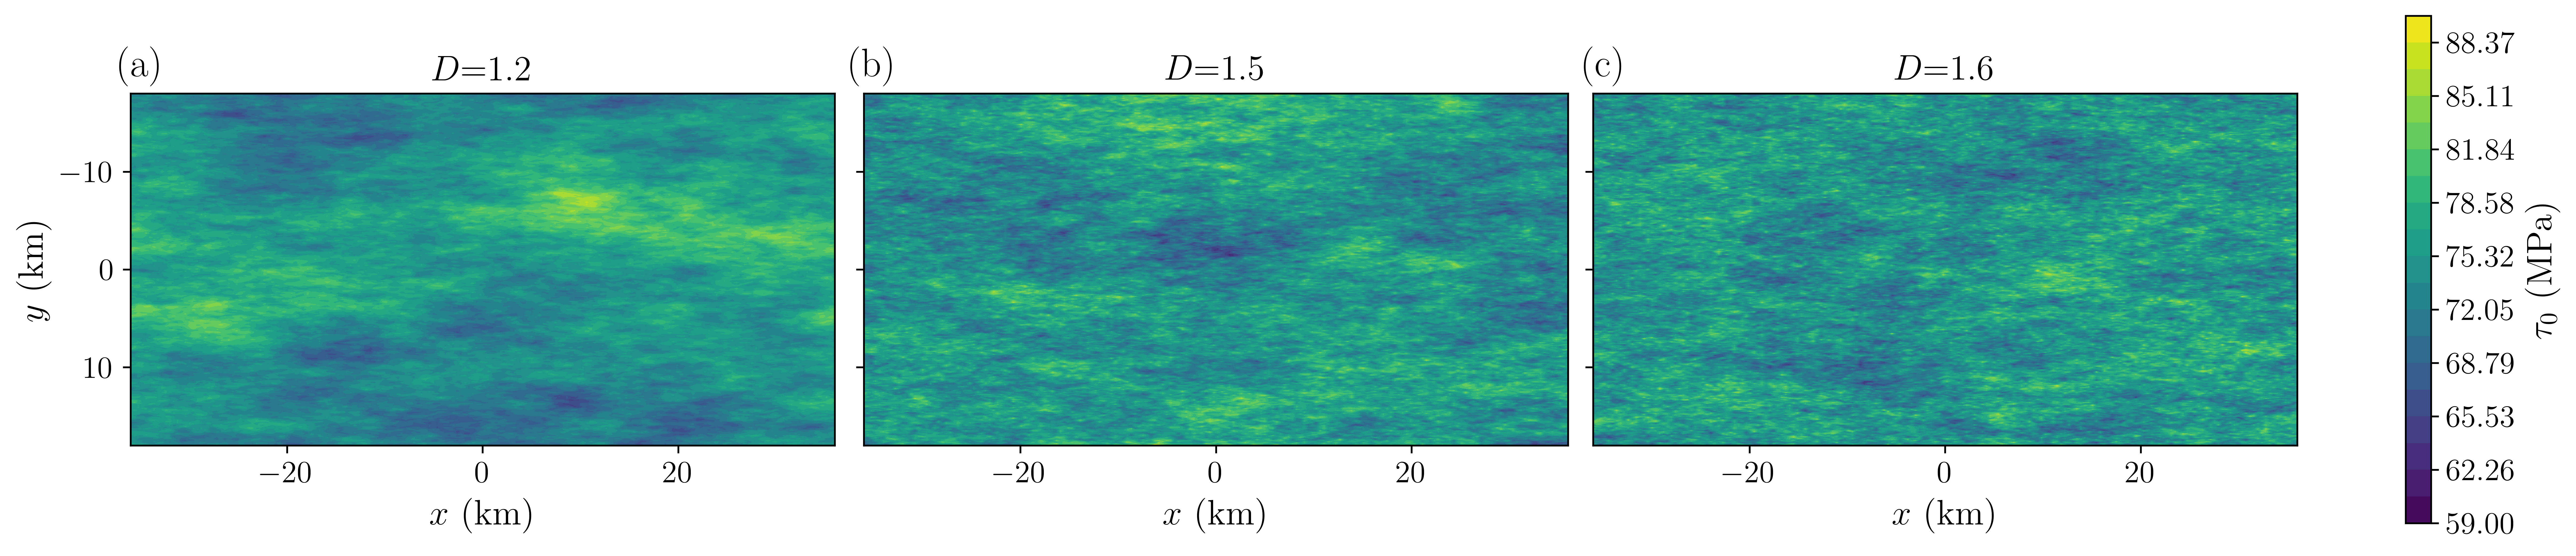
\includegraphics[width=1.0\linewidth]{3D_input_contour.png}
\caption{\label{fig:3D_contour}Initial fractal shear stress distributions \(\tau_{0}\) with fractal dimensions of (a) 1.2, (b) 1.5, and (c) 1.6. The target mean is set to 75 MPa, with a target standard deviation of 5 MPa.
}
\end{figure}

As in the 2D case, the FNO is trained to approximate the mapping from the initial shear stress \DIFdelbegin \DIFdel{and }\DIFdelend \DIFaddbegin \DIFadd{\(\Delta\tau_{zx0}\), slip rate \(V_{zx0}\), }\DIFaddend frictional parameters \( a \) and \( b \)\DIFaddbegin \DIFadd{, and stress perturbation \(\Delta\tau_{zx}\) }\DIFaddend to the sequence of \DIFdelbegin \DIFdel{slip rates }\DIFdelend \DIFaddbegin \DIFadd{component of slip rates \(V_{zx}\) }\DIFaddend over the time interval of interest. The input data is structured as a tensor of dimensions \( (N, X, Y, C_{\text{in}}) \), while the output data has dimensions \( (N, X, Y, C_{\text{out}}) \), where \( X \) and \( Y \) represent the number of spatial discretization points in the \( x \) and \( y \) directions, respectively.

The \DIFdelbegin \DIFdel{two-dimensional }\DIFdelend \DIFaddbegin \DIFadd{2D }\DIFaddend fault is discretized into \( 720 \times 360 \) spatial points, i.e., \( X = 720 \) and \( Y = 360 \). The input channels consist of the spatial distributions of \DIFdelbegin \DIFdel{initial shear stress, parameter \( a \), and parameter \( b \), resulting in \( C_{\text{in}} = 3 \)}\DIFdelend \DIFaddbegin \DIFadd{\(\tau_0\), \(V_0\), \(a\), \(b\), and ten steps of \(\Delta\tau\), sampled from \(t=t_0\) to \(t = t_0 + 0.9\) s, resulting in \( C_{\text{in}} = 14 \)}\DIFaddend .

\DIFdelbegin \DIFdel{It is worth noting that the time step $\Delta t$ in the SBI solver is 0.01 }\DIFdelend \DIFaddbegin \DIFadd{The SBI solver uses a time step of \(\Delta t = 0.01\)~}\DIFaddend s to satisfy the CFL condition with \(\Delta x = \Delta y = 100\)\DIFdelbegin \DIFdel{m and \(f\) = 0.6. We output the SBI solution }\DIFdelend \DIFaddbegin \DIFadd{~m and \(f = 0.6\). Solutions are output }\DIFaddend at a frequency of 0.1\DIFdelbegin \DIFdel{s. The discretization consists of \( 720 \times 360 \) spatial points. This results in \( (N, X, Y, C_{\text{out}}) = (3600, 720, 360, 150) \), producing approximately 500 GB }\DIFdelend \DIFaddbegin \DIFadd{~s. For FNO training, we generate 60 time steps of \(V_{zx}\) evolution at 0.2~s intervals starting from \(t = t_0\), resulting in output dimensions \((N, X, Y, C_{\text{out}}) = (28700, 720, 360, 60)\), which corresponds to approximately 2~TB }\DIFaddend of data. Given the available memory and GPU limitations, training with a single batch at this scale is challenging. \DIFdelbegin \DIFdel{To address this}\DIFdelend \DIFaddbegin \DIFadd{Thus}\DIFaddend , we reduce the number of spatial and temporal points by sub-sampling from \DIFdelbegin \DIFdel{\( (X, Y, C_{\text{out}}) = (720, 360, 150)\) to \((360, 180, 76)\) }\DIFdelend \DIFaddbegin \DIFadd{\( (X, Y, C_{\text{out}}) = (720, 360, 60)\) to \((360, 180, 60)\) }\DIFaddend for FNO training, reducing the dataset size to approximately \DIFdelbegin \DIFdel{66 }\DIFdelend \DIFaddbegin \DIFadd{416 }\DIFaddend GB. In this case, the output channels correspond to snapshots of \DIFdelbegin \DIFdel{slip rate }\DIFdelend \DIFaddbegin \DIFadd{\(V_{zx}\) }\DIFaddend spatially sampled at half the resolution of the original simulations and temporally recorded at 0.2 s intervals\DIFdelbegin \DIFdel{, covering the time range \( t = 0 \) s to \( t = 15 \) s, thus \( C_{\text{out}} = 76 \)}\DIFdelend . This adjustment makes training feasible on the available NVIDIA A100 GPU with 64 GB of memory.

As with the 2D dataset, we also normalize the 3D dataset, scaling each feature in both the input and output to the range \([0,1]\). After training, the original physical scale is restored using an inverse transformation.


\section{Results}
\label{sec:results}

\subsection{FNO-1D for 2D Dynamic Rupture Dataset}
\label{sec:FNO-1D}


\subsubsection{Training and Testing Performance}
\label{sec:FNO-1D_training}

We optimize the hyperparameters of FNO-1D, including the number of modes, Fourier layers, lifting and projection layers, and the learning rate. Details of hyperparameter tuning and training strategies are listed in Appendix \ref{sec:appendix_b}. The model selection criterion balances accuracy with computational efficiency by maintaining a minimal number of parameters. Based on this tuning process, we configure the model with four Fourier layers (\(m = 4\)), while the lifting network \(P\) and projection network \(Q\) each consist of 128 neurons. The number of retained modes after applying the Fourier transform and subsequent linear transformation is set to 16. The activation function \DIFdelbegin \DIFdel{employed }\DIFdelend is the Gaussian Error Linear Unit (GELU) \cite{hendrycks2016gaussian}. The model is trained using a batch size of 10, with a relative \(L_2\) loss function and the Adam optimizer \cite{kingma2014adam}, adopting a learning rate of \(10^{-3}\) and a weight decay of \(10^{-4}\) with a cosine annealing schedule. The training process is conducted for \DIFdelbegin \DIFdel{10,000 }\DIFdelend \DIFaddbegin \DIFadd{500 }\DIFaddend epochs. The training and testing losses are shown in Figure \ref{fig:loss}\DIFaddbegin \DIFadd{a}\DIFaddend . Both training and testing losses consistently decrease without \DIFdelbegin \DIFdel{significant }\DIFdelend \DIFaddbegin \DIFadd{large }\DIFaddend divergence between them, indicating no signs of overfitting.
\DIFdelbegin \DIFdel{Some fluctuations in the testing loss at the beginning occur due to the selected batch size.
}\DIFdelend 

\begin{figure}
\centering
\DIFdelbeginFL %DIFDELCMD < 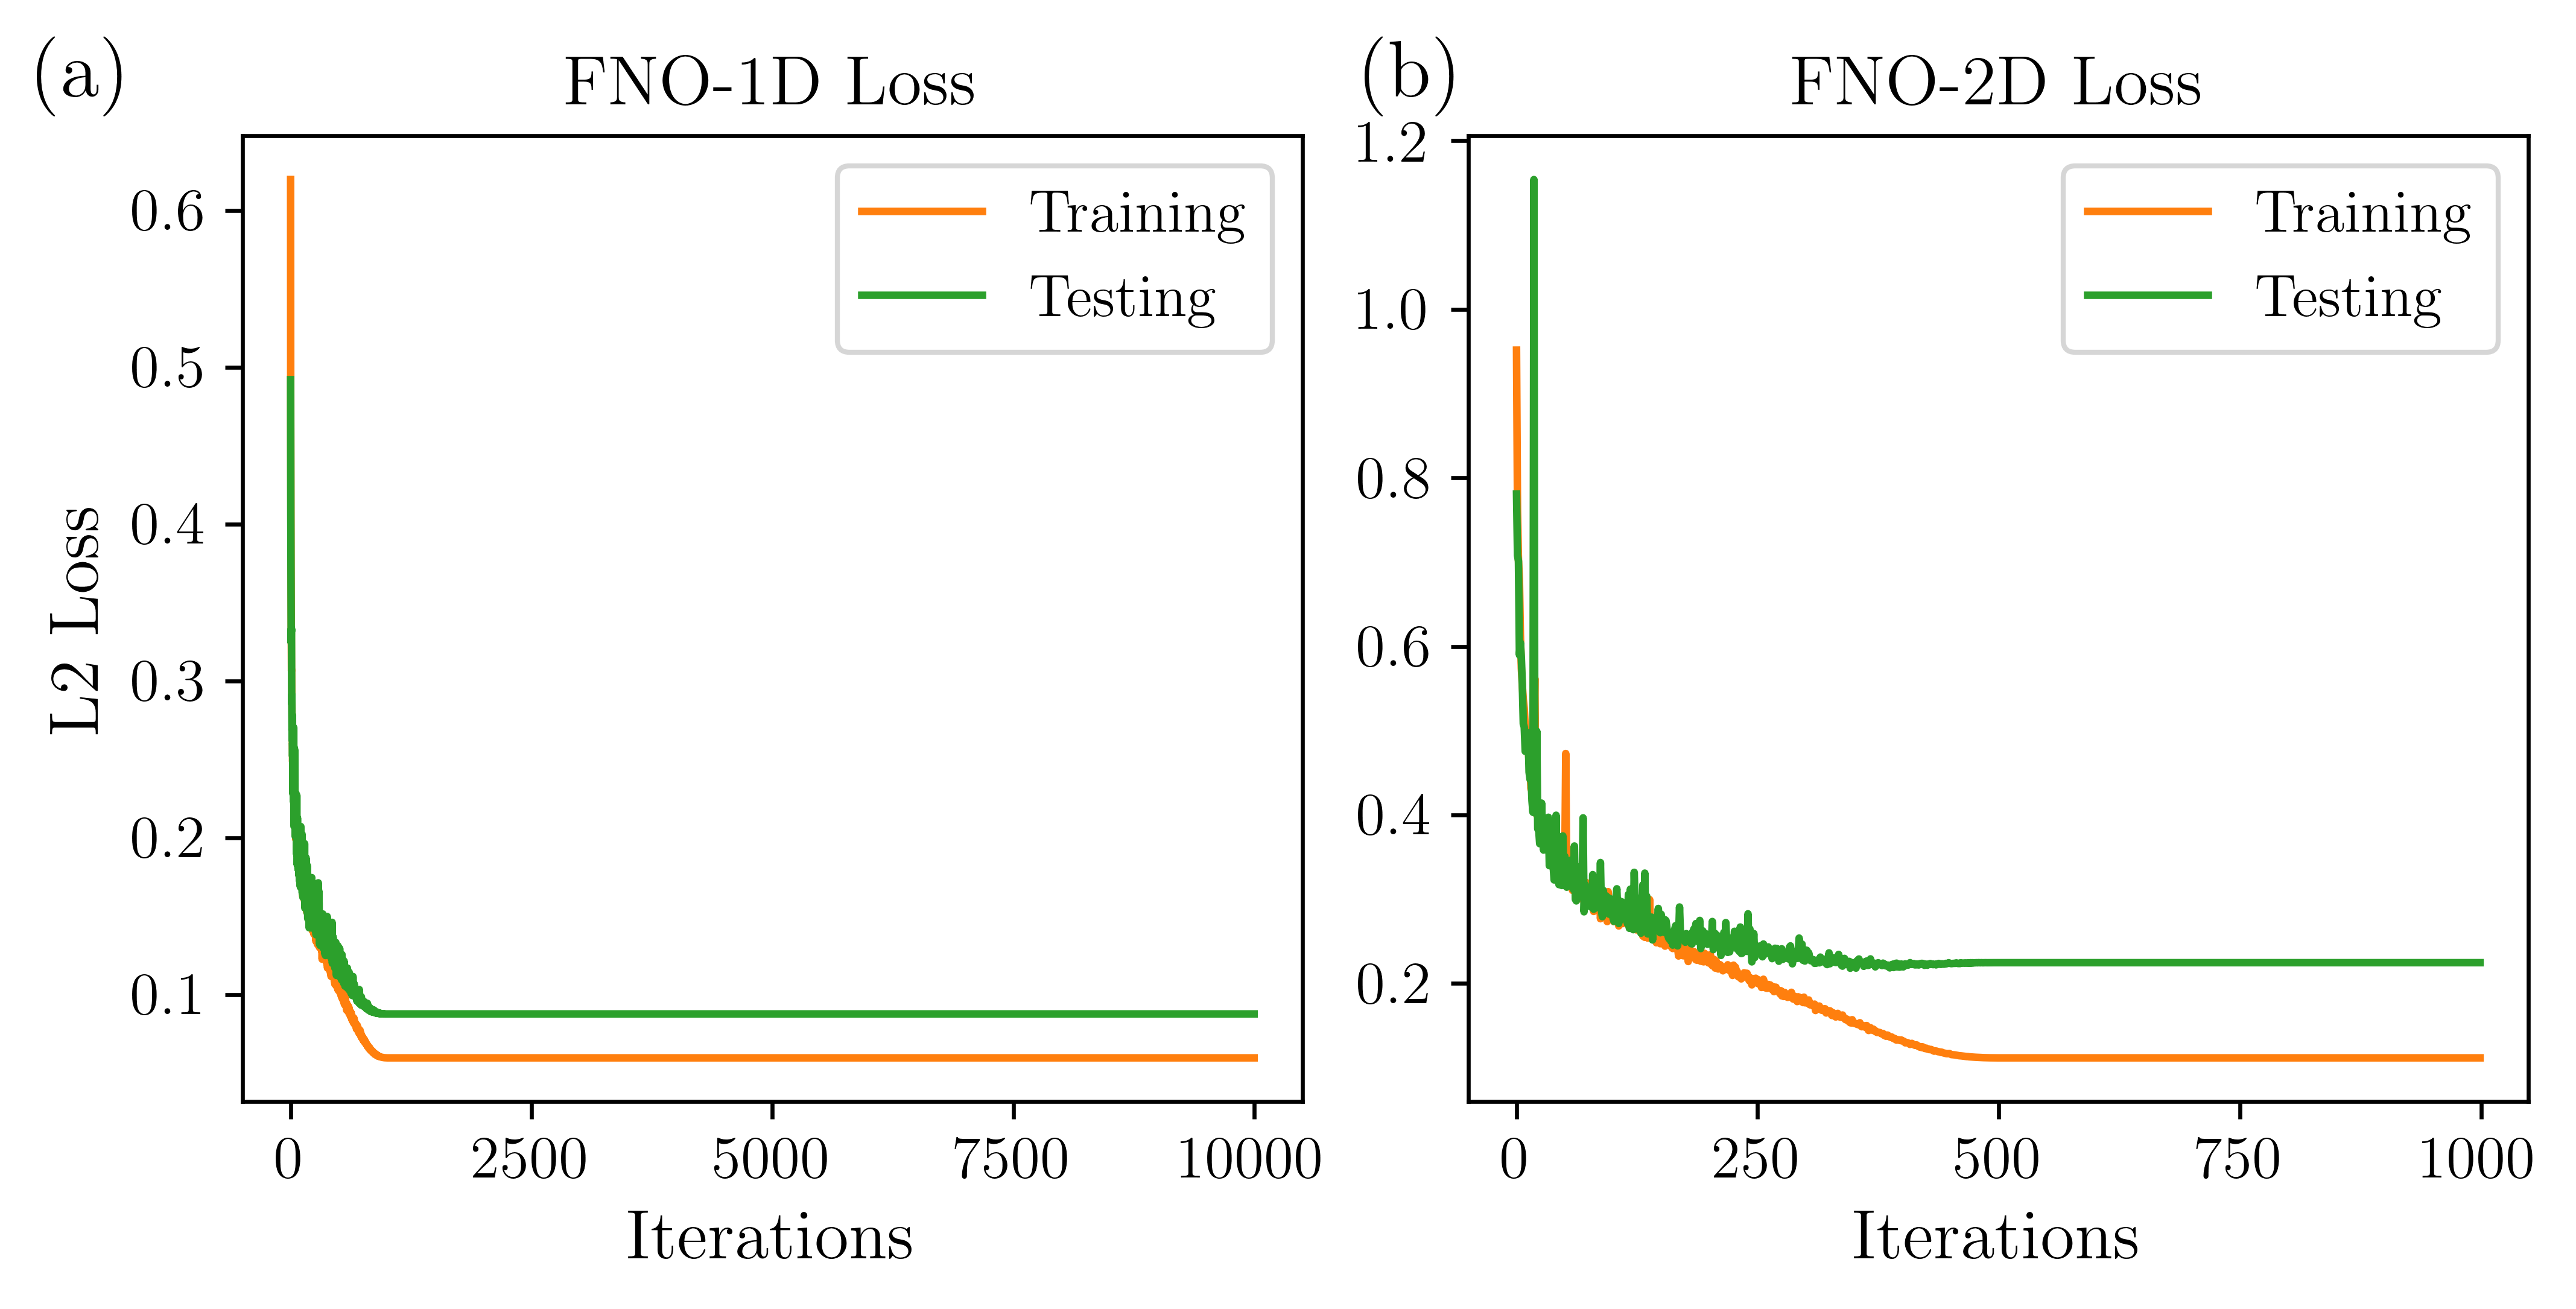
\includegraphics[width=0.7\linewidth]{loss2.png}
%DIFDELCMD < %%%
\DIFdelendFL \DIFaddbeginFL 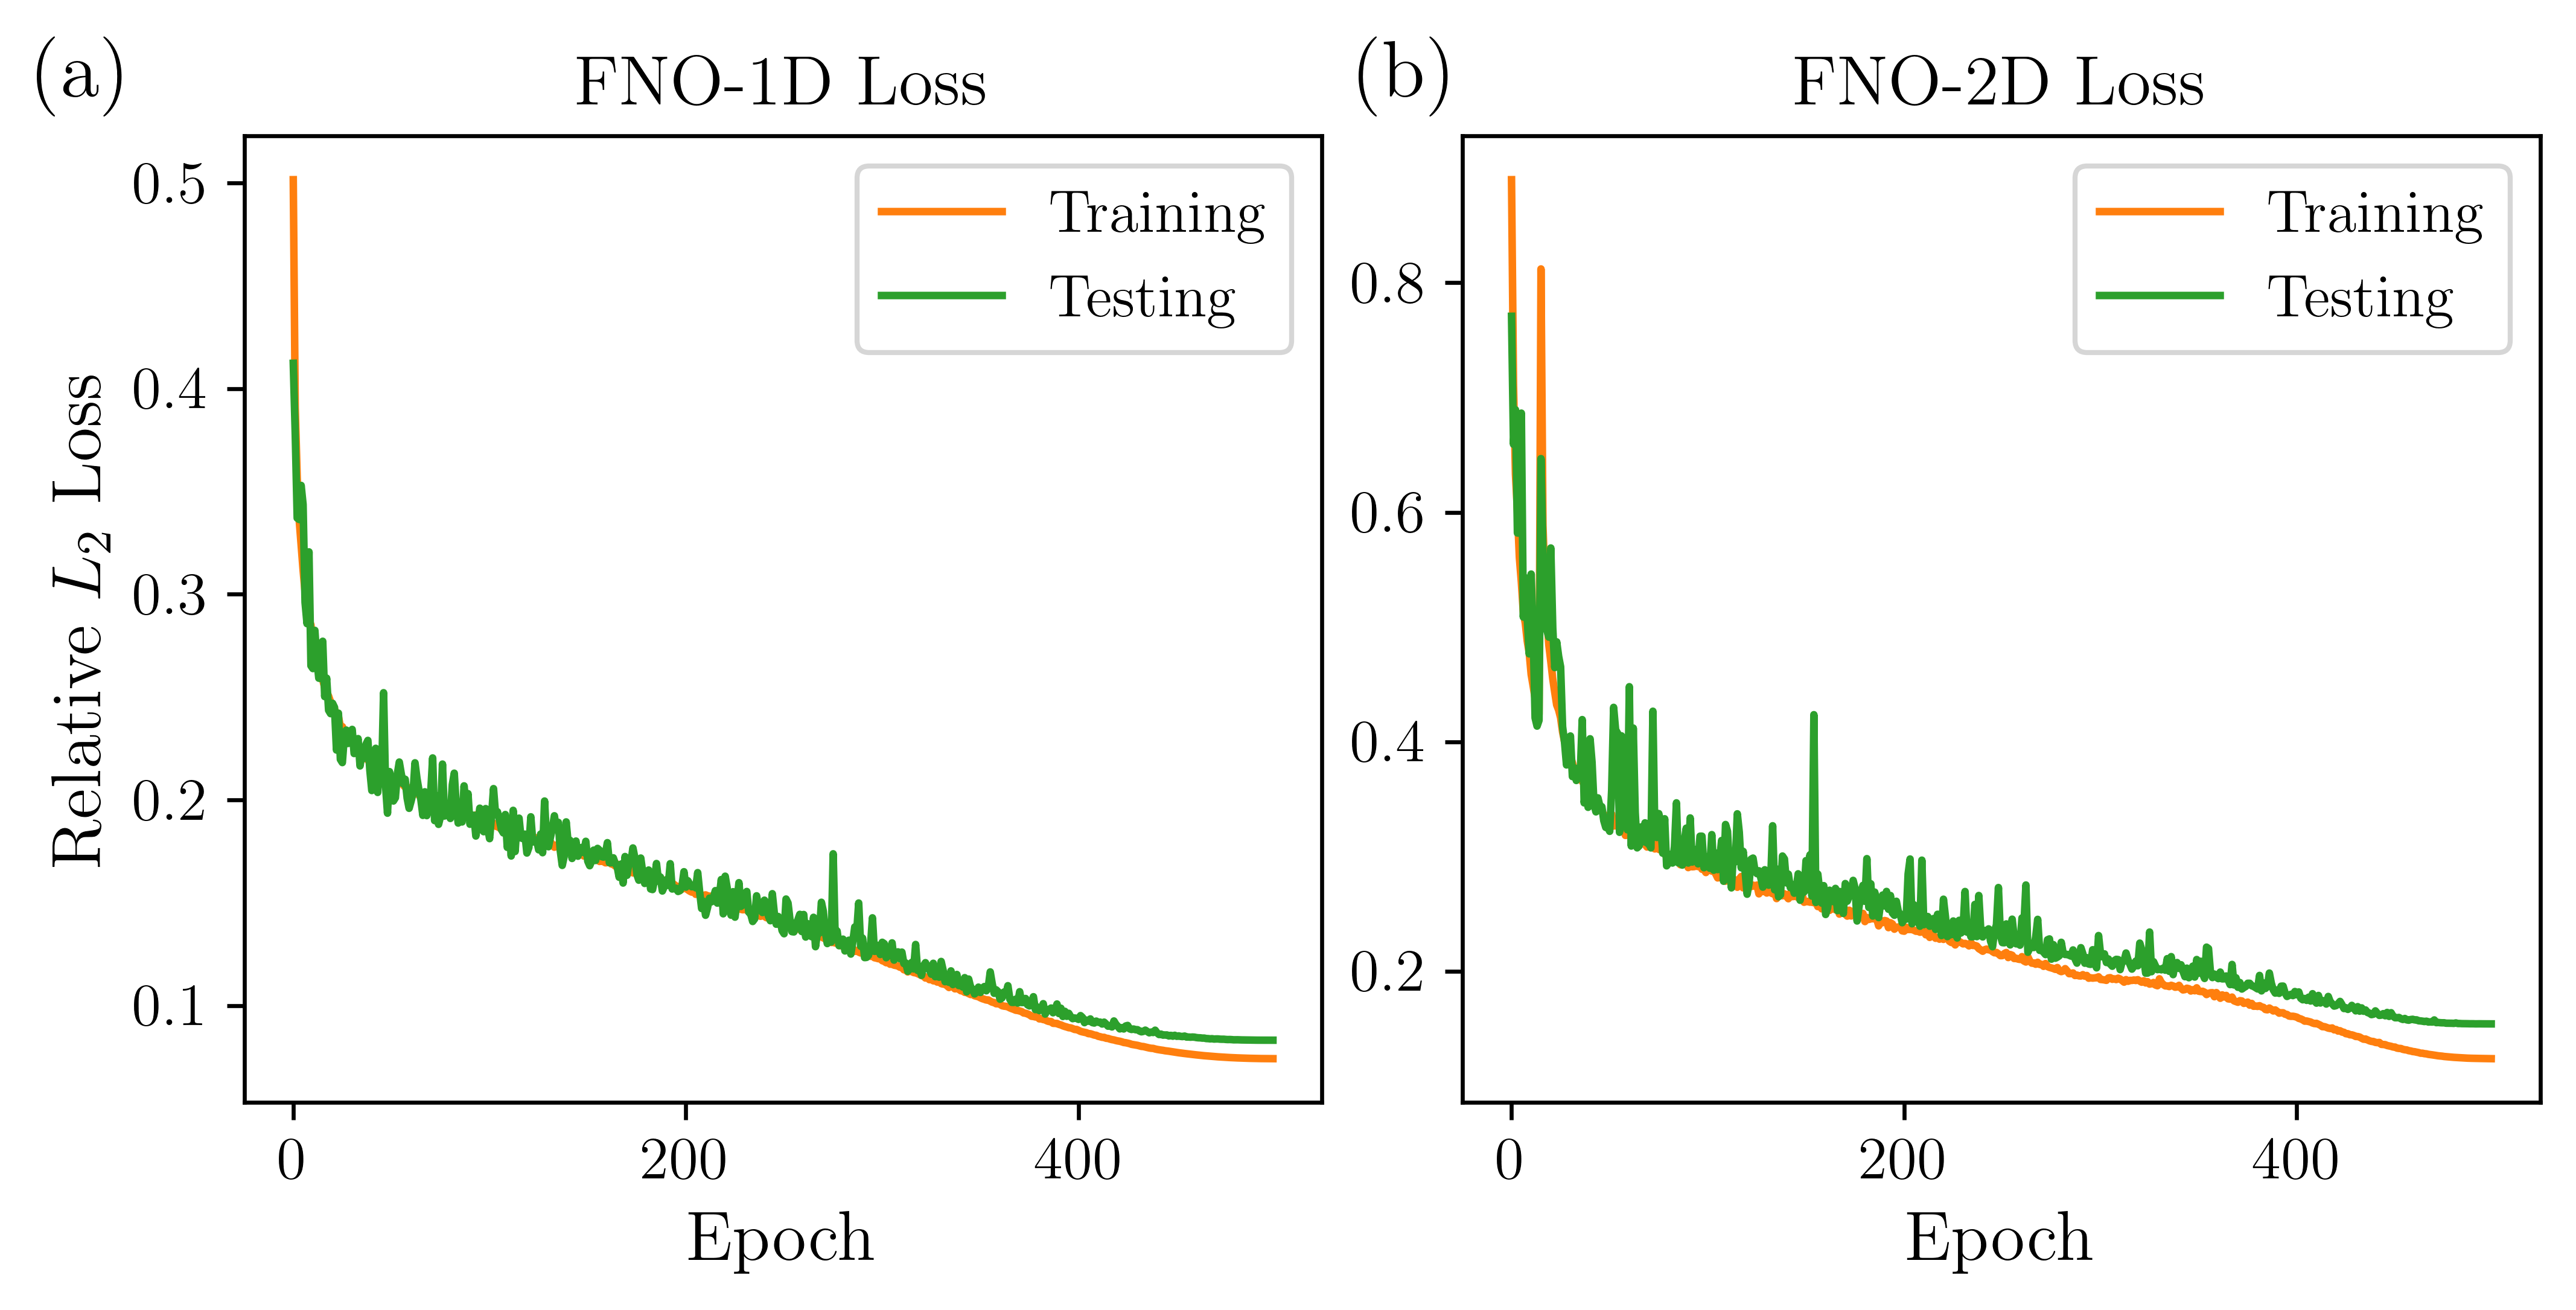
\includegraphics[width=0.7\linewidth]{loss.png}
\DIFaddendFL \caption{\label{fig:loss}Training and testing losses for (a) 2D dynamic rupture dataset and (b) 3D dynamic rupture dataset.
}
\end{figure}

The performance of FNO-1D is evaluated on the testing dataset. The model predictions, compared against the ground truth, are presented in Figure \ref{fig:fno_1D_test}. FNO-1D effectively captures a wide range of magnitudes arising from different distributions of \(\tau_{0}\)\DIFdelbegin \DIFdel{and the frictional parameters }\DIFdelend \DIFaddbegin \DIFadd{, \(V_{0}\), \(\Delta \tau\), }\DIFaddend \(a\)\DIFaddbegin \DIFadd{, }\DIFaddend and \(b\). The model successfully reproduces the global slip rate, particularly in regions characterized by sharp gradients, such as the rupture front. Discrepancies arise in regions where resolving closely spaced high-frequency components is required. These features reflect a phenomenon known as spectral bias \cite{rahaman2019spectral, cao2019towards, kong2025reducing}, which implies that deep learning models predict high-frequency features less accurately than lower-frequency ones. In \DIFdelbegin \DIFdel{Appendix }\DIFdelend \ref{sec:appendix_b}, we discuss a potential strategy for improving the model's performance \DIFdelbegin \DIFdel{at higher frequencies by implementing a specialized training protocol}\DIFdelend \DIFaddbegin \DIFadd{by training on more datasets}\DIFaddend .


\begin{figure}
\centering
\DIFdelbeginFL %DIFDELCMD < \includegraphics[width=1.0\linewidth]{2D_best_pred_test.png}
%DIFDELCMD < %%%
\DIFdelendFL \DIFaddbeginFL \includegraphics[width=1.0\linewidth]{2D_pred_test.png}
\DIFaddendFL \caption{\label{fig:fno_1D_test}Testing of the trained FNO-1D model on the 2D dynamic rupture \DIFdelbeginFL \DIFdelFL{test }\DIFdelendFL dataset\DIFdelbeginFL \DIFdelFL{: }\DIFdelendFL \DIFaddbeginFL \DIFaddFL{.  
}\DIFaddendFL (a) Inputs include \DIFaddbeginFL \DIFaddFL{the }\DIFaddendFL initial fractal shear stress \DIFdelbeginFL \DIFdelFL{distributions \(\tau_{0}\) and (b) }\DIFdelendFL \DIFaddbeginFL \DIFaddFL{distribution \(\tau_0\) with \(D = 1.2\), initial slip rate at the time step where \(\max(V) > V_{\text{th}}\) with \(V_{\text{th}} = 1e-2\), }\DIFaddendFL frictional parameters \(a\) and \(b\) \DIFdelbeginFL \DIFdelFL{; (c) Outputs consist }\DIFdelendFL \DIFaddbeginFL \DIFaddFL{where \(a_0 = 0.0065\), \(\Delta a_0 = 0.011\), and \(b = 0.012\), and 10 steps }\DIFaddendFL of \DIFaddbeginFL \DIFaddFL{stress perturbation \(\Delta \tau\) starting from the same thresholded step. The outputs are }\DIFaddendFL predicted slip rate snapshots at selected \DIFdelbeginFL \DIFdelFL{discrete }\DIFdelendFL time steps \DIFaddbeginFL \DIFaddFL{following this point (rows 3--7)}\DIFaddendFL .  
\DIFaddbeginFL \DIFaddFL{(b--d) Same as (a), but with varying conditions:  
(b) \(D = 1.5\), \(a_0 = 0.006\), \(\Delta a_0 = 0.012\), \(b = 0.014\), \(V_{\text{th}} = 10^{-4}\);  
(c) \(D = 1.5\), \(a_0 = 0.009\), \(\Delta a_0 = 0.006\), \(b = 0.012\), \(V_{\text{th}} = 10^{-2}\);  
(d) \(D = 1.6\), \(a_0 = 0.007\), \(\Delta a_0 = 0.010\), \(b = 0.012\), \(V_{\text{th}} = 10^{-3}\).  
In all cases, predictions are generated starting from the time step where the slip rate exceeds the specified threshold.
}\DIFaddendFL }
\end{figure}

\begin{table}
\caption{Median and median absolute deviation (MAD) of NRMSE and relative \(L_2\) error in the bracket shown in Figure \ref{fig:l2} for \DIFdelbeginFL \DIFdelFL{3600 }\DIFdelendFL \DIFaddbeginFL \DIFaddFL{28,700 }\DIFaddendFL training samples and \DIFdelbeginFL \DIFdelFL{400 }\DIFdelendFL \DIFaddbeginFL \DIFaddFL{4,100 }\DIFaddendFL testing samples of 2D and 3D dynamic rupture datasets.}
    \centering
    { % Resize table to fit within text width
    \begin{tabular}{lll}
        \toprule
        \multirow{3}{*}{} & \multicolumn{1}{c}{\textbf{2D Dynamic Rupture}} & \multicolumn{1}{c}{\textbf{3D Dynamic Rupture}} \\
        & \multicolumn{1}{c}{NRMSE} & \multicolumn{1}{c}{NRMSE} \\
        & \multicolumn{1}{c}{(Relative \( L_2 \) Error)} & \multicolumn{1}{c}{(Relative \( L_2 \) Error)} \\
        \midrule
        Training& \DIFdelbeginFL \DIFdelFL{0.00261 }\DIFdelendFL \DIFaddbeginFL \DIFaddFL{0.00357 }\DIFaddendFL $\pm$  \DIFdelbeginFL \DIFdelFL{0.000477 }\DIFdelendFL \DIFaddbeginFL \DIFaddFL{0.000957 }\DIFaddendFL & \DIFdelbeginFL \DIFdelFL{0.00231 }\DIFdelendFL \DIFaddbeginFL \DIFaddFL{0.00317 }\DIFaddendFL $\pm$  \DIFdelbeginFL \DIFdelFL{0.000377 }\DIFdelendFL \DIFaddbeginFL \DIFaddFL{0.000612 }\DIFaddendFL \\
         & (\DIFdelbeginFL \DIFdelFL{0.0550 }\DIFdelendFL \DIFaddbeginFL \DIFaddFL{0.0665 }\DIFaddendFL $\pm$  \DIFdelbeginFL \DIFdelFL{0.00966}\DIFdelendFL \DIFaddbeginFL \DIFaddFL{0.01581}\DIFaddendFL ) & (\DIFdelbeginFL \DIFdelFL{0.0854 }\DIFdelendFL \DIFaddbeginFL \DIFaddFL{0.115 }\DIFaddendFL $\pm$ \DIFdelbeginFL \DIFdelFL{0.0129}\DIFdelendFL \DIFaddbeginFL \DIFaddFL{0.0239}\DIFaddendFL ) \\
        Testing & \DIFdelbeginFL \DIFdelFL{0.00329 }\DIFdelendFL \DIFaddbeginFL \DIFaddFL{0.00388 }\DIFaddendFL $\pm$  \DIFdelbeginFL \DIFdelFL{0.000852 }\DIFdelendFL \DIFaddbeginFL \DIFaddFL{0.00114 }\DIFaddendFL &  \DIFdelbeginFL \DIFdelFL{0.00387 }\DIFdelendFL \DIFaddbeginFL \DIFaddFL{0.00366 }\DIFaddendFL $\pm$  \DIFdelbeginFL \DIFdelFL{0.00132}\DIFdelendFL \DIFaddbeginFL \DIFaddFL{0.000940}\DIFaddendFL \\
         & (\DIFdelbeginFL \DIFdelFL{0.0685 }\DIFdelendFL \DIFaddbeginFL \DIFaddFL{0.0270 }\DIFaddendFL $\pm$ \DIFdelbeginFL \DIFdelFL{0.0209}\DIFdelendFL \DIFaddbeginFL \DIFaddFL{0.00909}\DIFaddendFL )  & (\DIFdelbeginFL \DIFdelFL{0.153 }\DIFdelendFL \DIFaddbeginFL \DIFaddFL{0.133 }\DIFaddendFL $\pm$ \DIFdelbeginFL \DIFdelFL{0.0514}\DIFdelendFL \DIFaddbeginFL \DIFaddFL{0.0368}\DIFaddendFL ) \\
        \bottomrule
    \end{tabular}
    }
    \label{tab:relative_l2_error}
\end{table}


We summarize the NRMSE and relative \(L_2\) error on the training and testing datasets in Figure \ref{fig:l2}. Testing samples show slightly higher errors but still follow the same distribution as the training set, suggesting no major overfitting. The majority of samples have small errors and are highly skewed towards zero, with the median and median absolute deviation (MAD) of the errors presented in Table \ref{tab:relative_l2_error}. According to Figure~\ref{fig:l2}b, more than \DIFdelbegin \DIFdel{90}\DIFdelend \DIFaddbegin \DIFadd{95}\DIFaddend \(\%\) of the training set shows a relative \(L_2\) error of less than 10\(\%\), while this fraction drops to \DIFdelbegin \DIFdel{80}\DIFdelend \DIFaddbegin \DIFadd{90}\DIFaddend \(\%\) for the testing set. \DIFaddbegin \DIFadd{This level of the error suggests that the model generalizes well to unseen data. }\DIFaddend Examples of the predictions corresponding to different selected values of the relative \(L_2\) error are presented in the supplementary information.

\begin{figure}
\centering
\DIFdelbeginFL %DIFDELCMD < 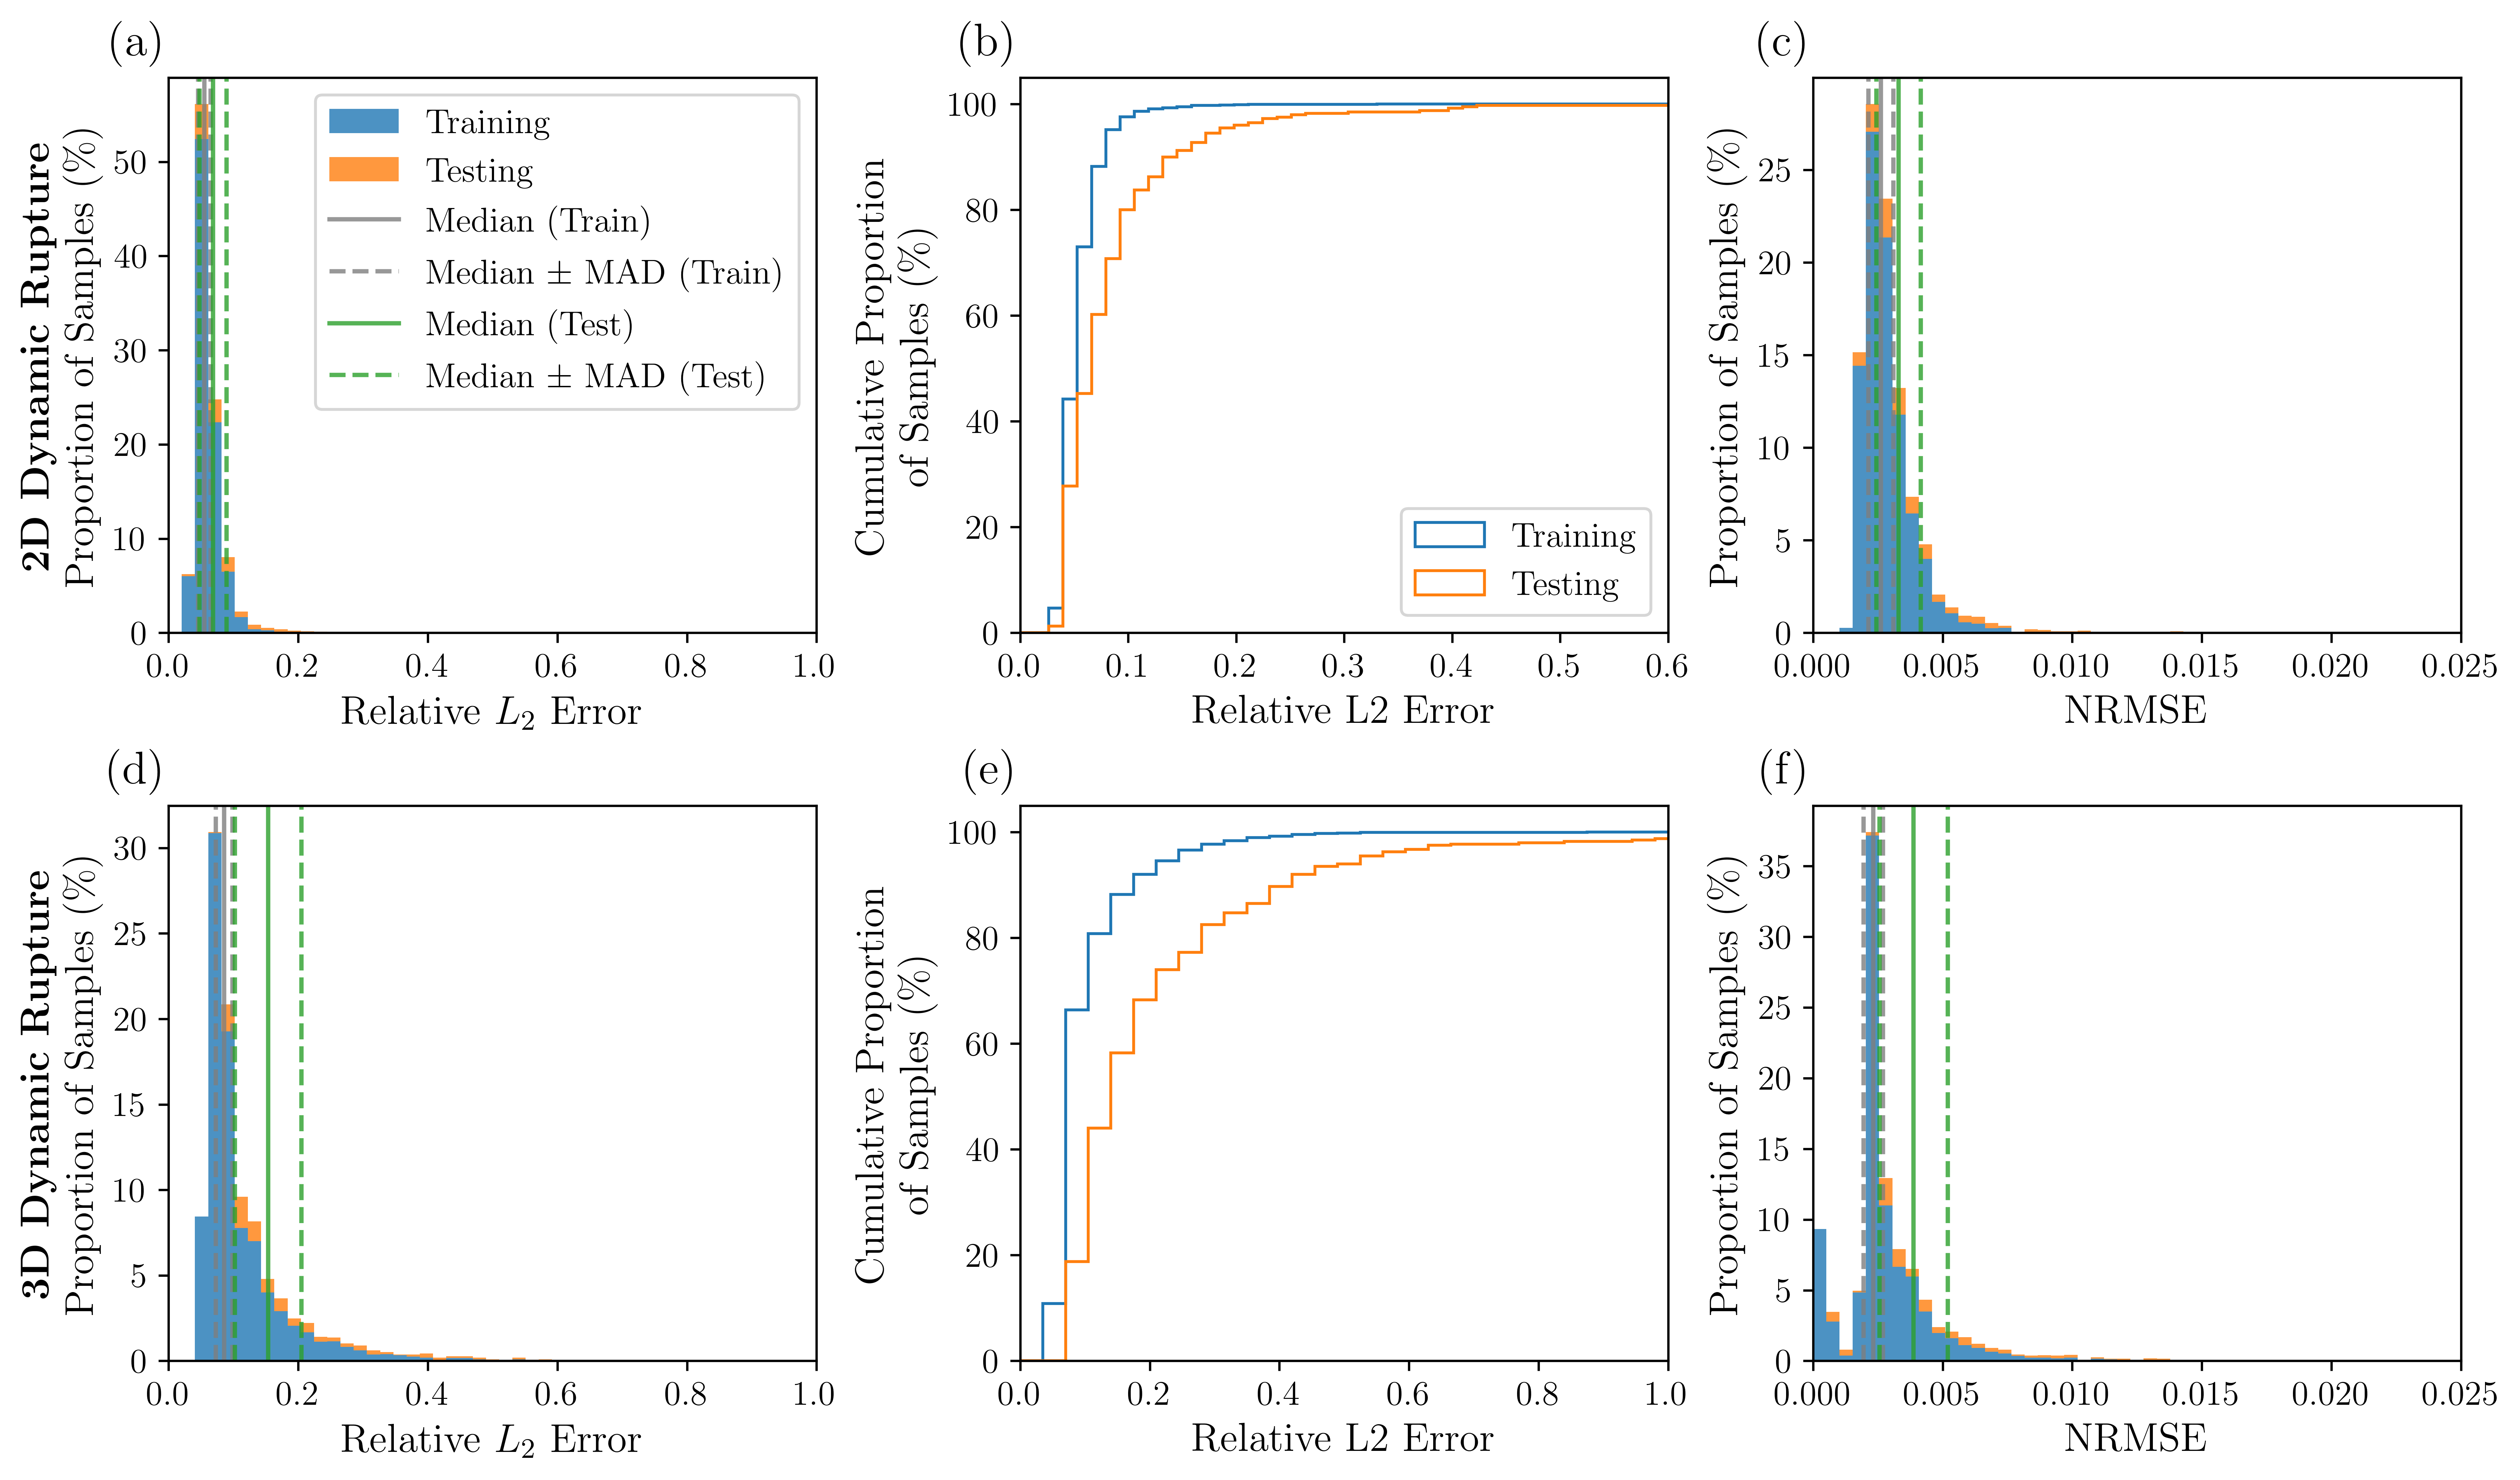
\includegraphics[width=0.9\linewidth]{stats_R3.png}
%DIFDELCMD < %%%
\DIFdelendFL \DIFaddbeginFL 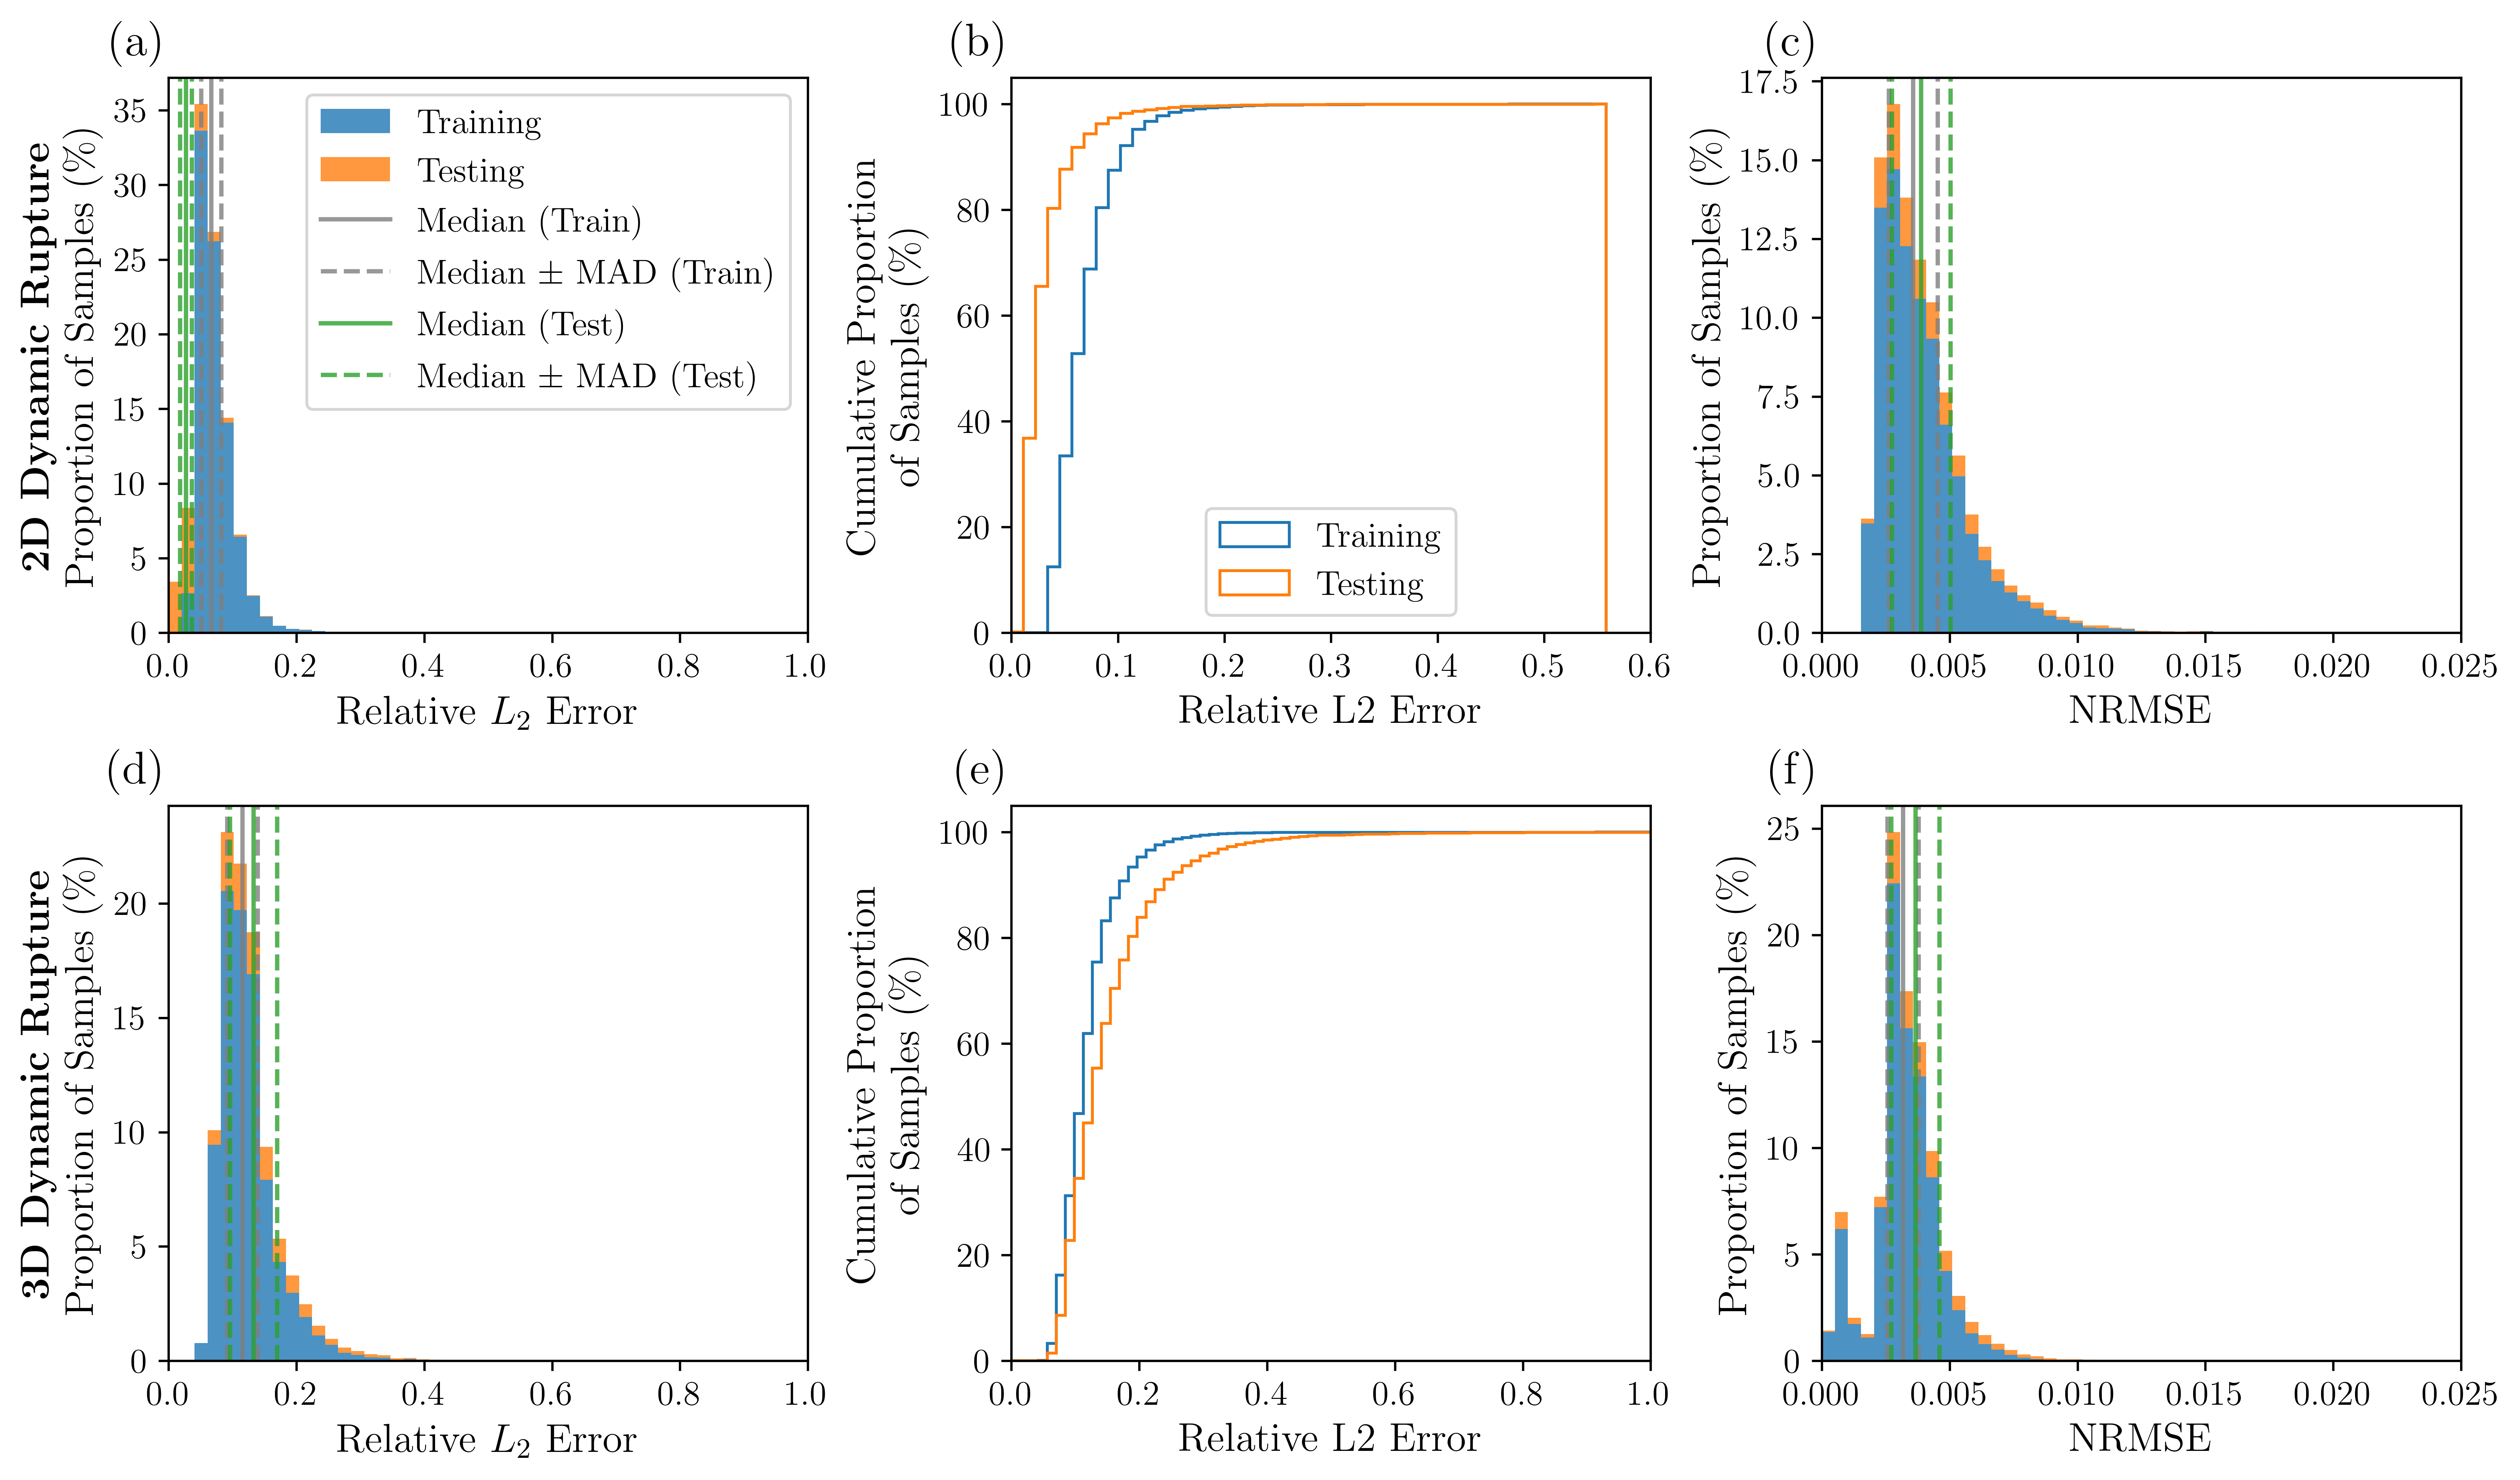
\includegraphics[width=0.9\linewidth]{stats.png}
\DIFaddendFL \caption{\label{fig:l2}Error analysis for 2D and 3D dynamic rupture predictions. (a) and (d) show histograms of the relative $L_2$ error distributions for the training (blue) and testing (orange) datasets in the 2D and 3D cases, respectively. Similarly, (c) and (f) show histograms of the NRMSE distributions for the training (blue) and testing (orange) datasets in the 2D and 3D cases. The vertical lines indicate the median error for the training (gray solid) and testing (green solid) datasets, as well as the median $\pm$ median absolute deviation (MAD) range for the training (gray dashed) and testing (green dashed) datasets. (b) and (e) show the cumulative histograms of the relative $L_2$ error distributions for the training (blue) and testing (orange) datasets in the 2D and 3D cases, respectively.
}
\end{figure}


\subsubsection{Generalization to Unseen Initial Shear Stress}
\label{sec:FNO-1D_unseen_shear}

An advantage of FNOs is that they can target the underlying operator, and learn to handle a family of problems rather than a single instance. Accordingly, in this section we test the generalization of our trained operator to some unseen initial conditions.

We evaluate the trained FNO-1D model, originally trained on initial fractal shear stress \(\tau_{0}\), using a uniform initial shear stress consistent with TPV101 problem description \cite{harris2018suite, harris2009scec, kammer2021uguca}. The initial shear stress of \(\tau_{0} = 75\) MPa is prescribed along the entire fault. This value is within the range of shear stress values in the fractal dataset. However, the network has not seen a spatially uniform case before this test. We compare predictions from the FNO-1D model against the ground truth in Figure \ref{fig:2D_benchmark}. The computed NRMSE and relative \(L_2\) error between the predictions and ground truth are \DIFdelbegin \DIFdel{0.00963 and 0.1822}\DIFdelend \DIFaddbegin \DIFadd{0.00560 and 0.0381}\DIFaddend , respectively. FNO-1D shows ability to capture slip rate evolution, particularly during rupture propagation in the VW regime and transitioning into the VS region. We observe \DIFdelbegin \DIFdel{noise, spatial shifts in the predictions, and }\DIFdelend \DIFaddbegin \DIFadd{minor noise near the rupture front in the predicted solution, along with }\DIFaddend slight mismatches in peak magnitudes at later times. \DIFdelbegin \DIFdel{Such discrepancies contribute to the high relative \(L_2\) error. }\DIFdelend However, the global features of slip rate remains consistent with the ground truth. These results highlight the robustness of FNO-1D, as the model successfully generalizes to this unseen distribution of \(\tau_{0}\).

\begin{figure}
\centering
\DIFdelbeginFL %DIFDELCMD < \includegraphics[width=1.0\linewidth]{2D_SCEC.png}
%DIFDELCMD < %%%
\DIFdelendFL \DIFaddbeginFL \includegraphics[width=1.0\linewidth]{2D_scec.png}
\DIFaddendFL \caption{\label{fig:2D_benchmark}Results of FNO-1D testing on an unseen shear stress distribution from the TPV101 SCEC/USGS benchmark\DIFaddbeginFL \DIFaddFL{. Panels (a) and (b) show selected input features}\DIFaddendFL : (a) \DIFdelbeginFL \DIFdelFL{Inputs include }\DIFdelendFL a uniform initial shear stress \DIFdelbeginFL \DIFdelFL{(\(\tau_{0}\)) of 75 }\DIFdelendFL \DIFaddbeginFL \DIFaddFL{\(\tau_0 = 75\)~}\DIFaddendFL MPa\DIFaddbeginFL \DIFaddFL{, }\DIFaddendFL and \DIFaddbeginFL \DIFaddFL{(b) the }\DIFaddendFL frictional parameters \(a\) and \(b\), with \DIFdelbeginFL \DIFdelFL{\(\Delta a_{0} = 0.008\) }\DIFdelendFL \DIFaddbeginFL \DIFaddFL{\(a_0 = 0.008\), \(\Delta a_0 = 0.008\), }\DIFaddendFL and \DIFdelbeginFL \DIFdelFL{\(a_{0} = 0.008\); }\DIFdelendFL \DIFaddbeginFL \DIFaddFL{\(b=0.012\). Other model inputs }\DIFaddendFL (\DIFdelbeginFL \DIFdelFL{b}\DIFdelendFL \DIFaddbeginFL \DIFaddFL{e.g., initial slip rate \(V_0\) with  a threshold \(V_\text{th} = 0\)~m/s and nucleation stress perturbation \(\Delta \tau\)}\DIFaddendFL ) \DIFdelbeginFL \DIFdelFL{Outputs }\DIFdelendFL \DIFaddbeginFL \DIFaddFL{are not shown. Panels (c)-(j) show the outputs }\DIFaddendFL consist of predicted slip rate profiles at selected time steps.
}
\end{figure}

Additionally, we \DIFdelbegin \DIFdel{test }\DIFdelend \DIFaddbegin \DIFadd{evaluate }\DIFaddend the performance of FNO-1D on an unseen fractal dimension \DIFdelbegin \DIFdel{\(D\). Specifically, we evaluate the trained model using a dataset generated with }\DIFdelend \(D = 1.3\), which was not \DIFdelbegin \DIFdel{part of }\DIFdelend \DIFaddbegin \DIFadd{included in }\DIFaddend the training set. \DIFdelbegin \DIFdel{In this case, the frictional parameter \(a\) follows a boxcar distribution, with \(a = 0.008\) in the VW region and \(a = 0.016\) in the VS region, while the frictional parameter \(b\) is fixed at \(0.012\).  
}\DIFdelend \DIFaddbegin \DIFadd{We generate 100 realizations with \(D = 1.3\) and randomly sampled frictional parameters from the ranges listed in Table~\ref{tab:dataset_summary}. After preprocessing the data using slip rate thresholds \(V_{\text{th}} \in \{0, 10^{-4}, 10^{-3}, 10^{-2}\}\), we obtain a total of 400 realizations for testing. The distribution of relative \(L_2\) error and NRMSE is shown in Figures~\ref{fig:2D_hist_unseen}a and ~\ref{fig:2D_hist_unseen}c. The distribution shows a high variance with some cases have relative \(L_2\) error close to 1.0. Expanding the training dataset is recommended to improve prediction accuracy.  
}

\DIFaddend Figure \ref{fig:2D_unseen_d} shows \DIFdelbegin \DIFdel{the }\DIFdelend \DIFaddbegin \DIFadd{an example of }\DIFaddend results from FNO-1D compared to the ground truth, with NRMSE and relative \(L_2\) error of \DIFdelbegin \DIFdel{0.00353 and 0.0566}\DIFdelend \DIFaddbegin \DIFadd{0.00254 and 0.0131}\DIFaddend , respectively. FNO-1D effectively captures both the low-frequency and high-frequency components of the slip rate \DIFdelbegin \DIFdel{up to approximately 12 }\DIFdelend \DIFaddbegin \DIFadd{with minor discrepancies at the peak at 12.3 }\DIFaddend s. The \DIFdelbegin \DIFdel{magnitude of the rupture front in the predictions also aligns with }\DIFdelend \DIFaddbegin \DIFadd{predicted rupture front also closely matches }\DIFaddend the ground truth \DIFdelbegin \DIFdel{. Some discrepancies occur when predicting the high-frequency component at later times}\DIFdelend \DIFaddbegin \DIFadd{during propagation into the VS region}\DIFaddend .  This test further corroborates the potential of FNO-1D in predicting slip rates under unseen initial shear stress conditions.

\begin{figure}
\centering
\DIFdelbeginFL %DIFDELCMD < \includegraphics[width=1.0\linewidth]{2D_fractal_dim13.png}
%DIFDELCMD < %%%
\DIFdelendFL \DIFaddbeginFL 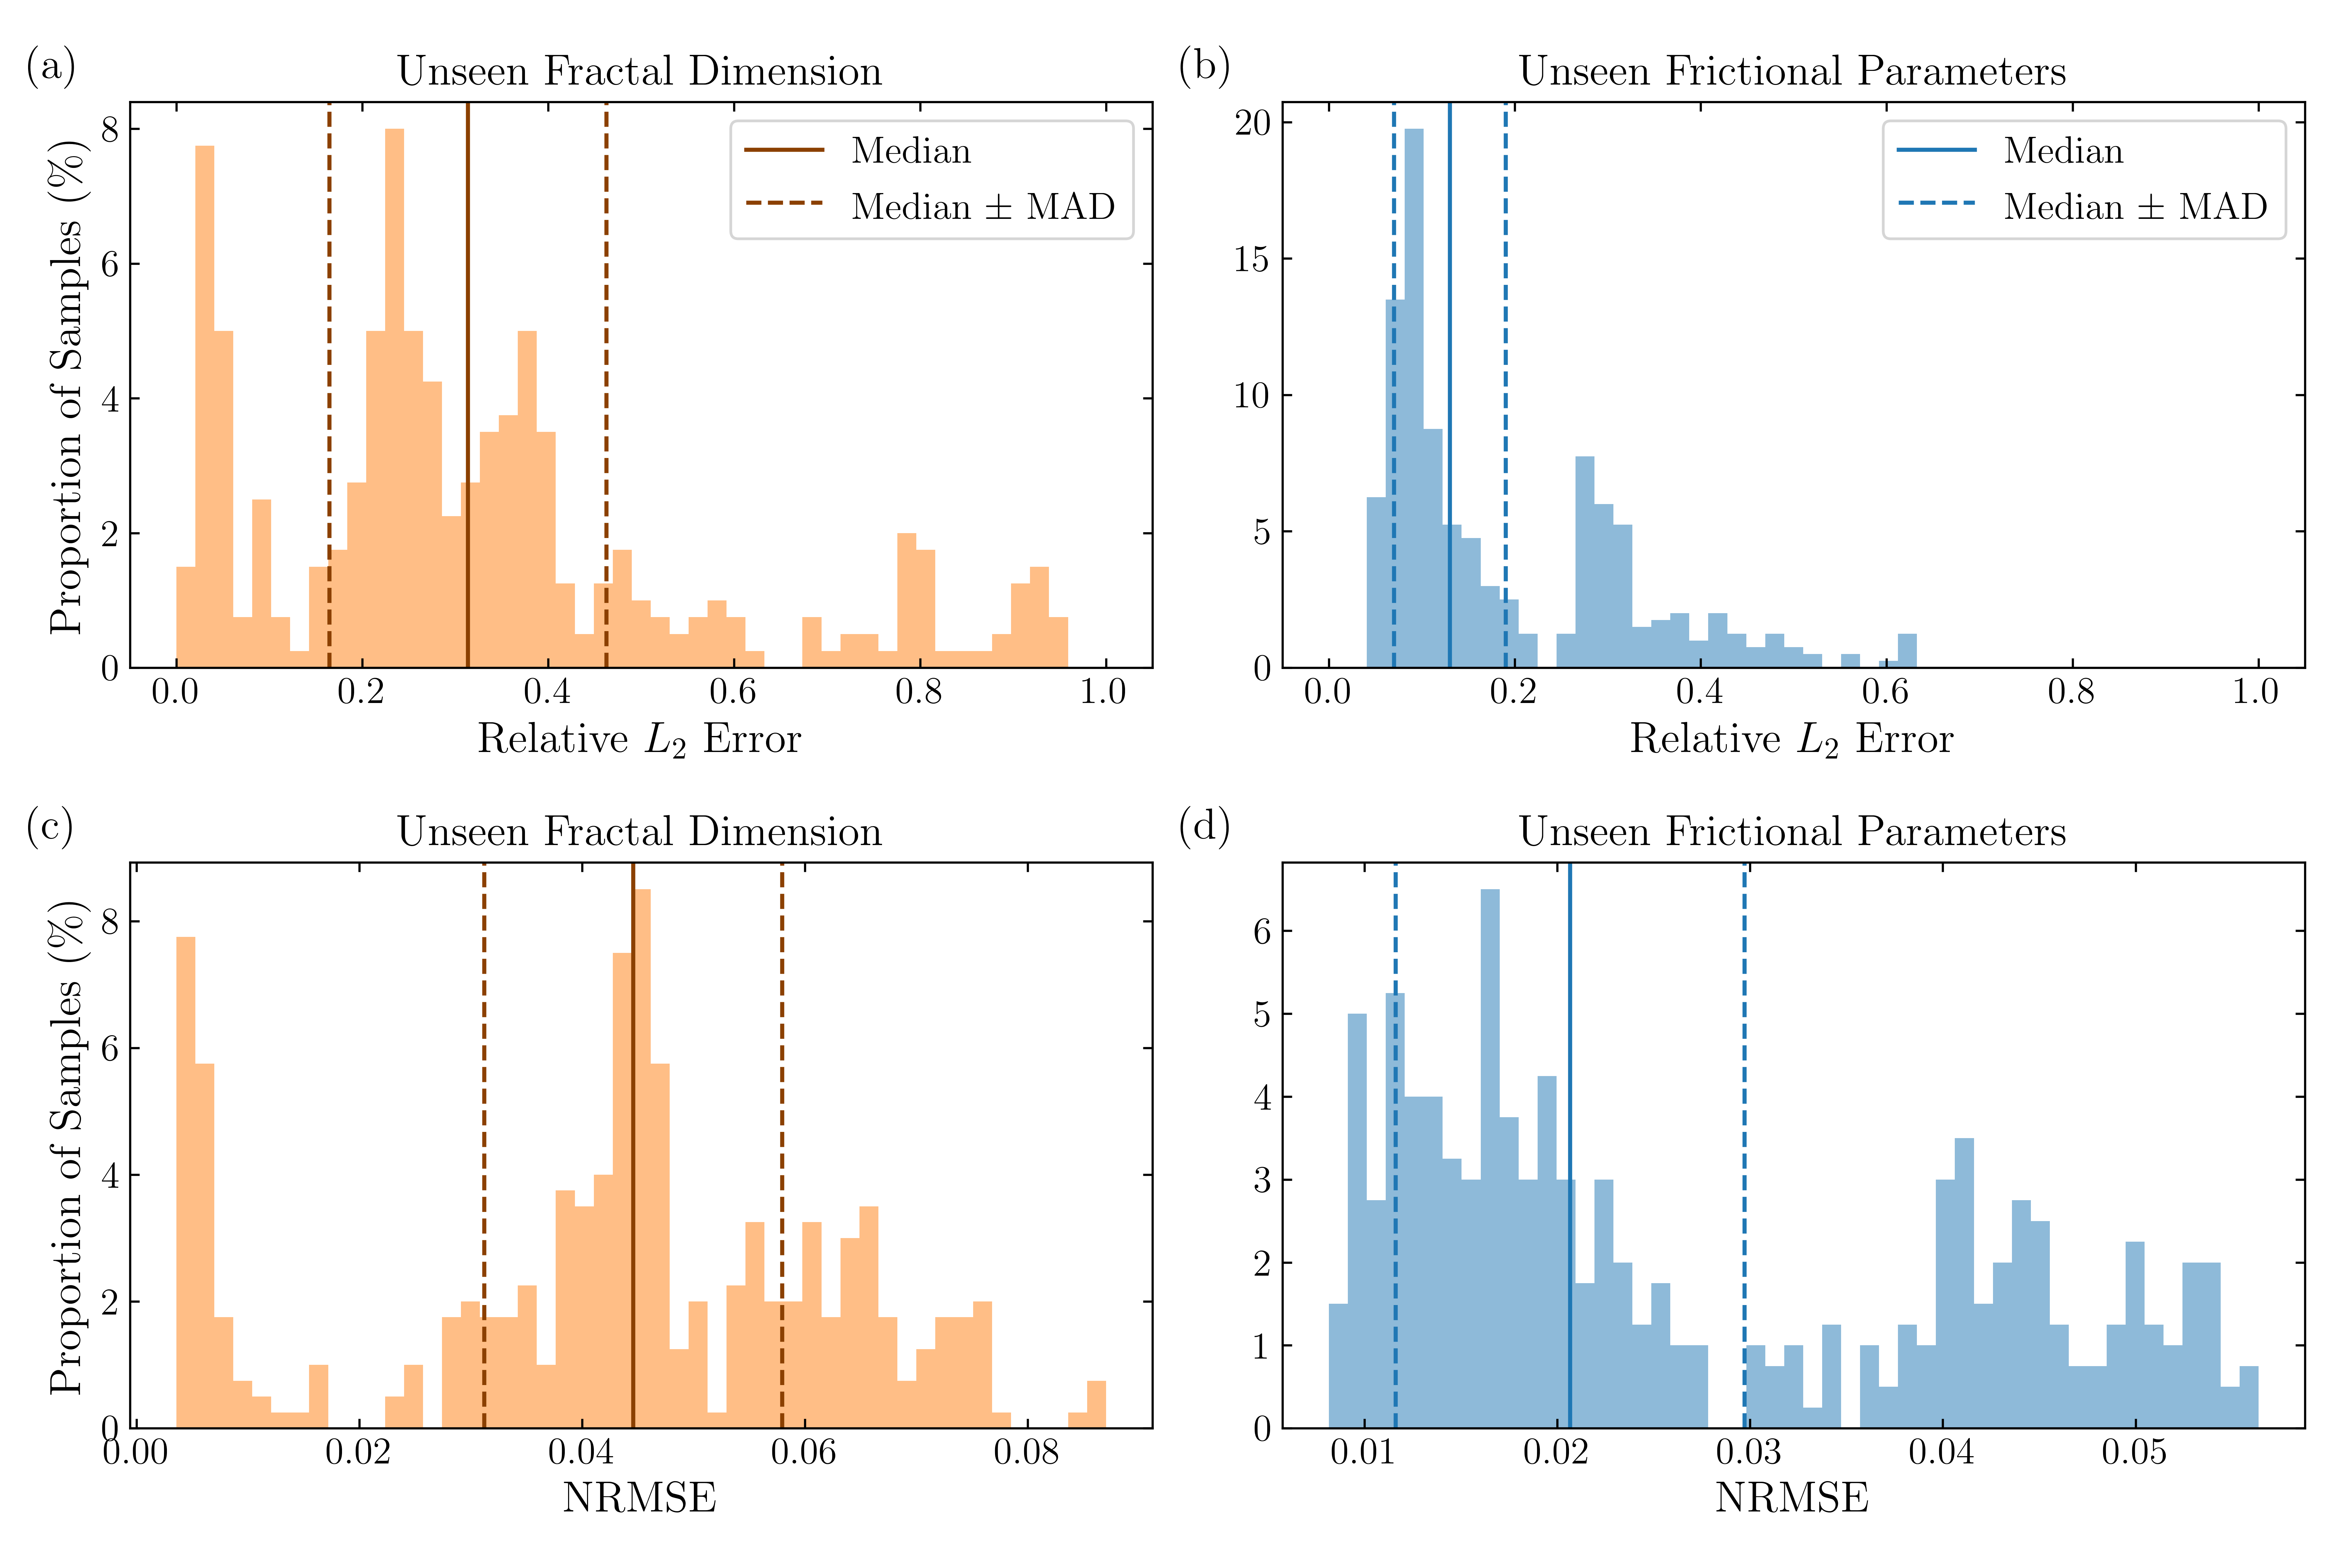
\includegraphics[width=1.0\linewidth]{2D_hist_unseen_2.png}
\DIFaddendFL \caption{\DIFdelbeginFL %DIFDELCMD < \label{fig:2D_unseen_d}%%%
\DIFdelFL{Results }\DIFdelendFL \DIFaddbeginFL \label{fig:2D_hist_unseen}\DIFaddFL{The distribution }\DIFaddendFL of \DIFdelbeginFL \DIFdelFL{FNO-1D testing on an unseen fractal dimension \(D = 1.3\): Inputs consist of }\DIFdelendFL (a) \DIFdelbeginFL \DIFdelFL{initial fractal shear stress distributions }\DIFdelendFL \DIFaddbeginFL \DIFaddFL{the relative \(L_2\) error and }\DIFaddendFL (\DIFdelbeginFL \DIFdelFL{\(\tau_{0}\)}\DIFdelendFL \DIFaddbeginFL \DIFaddFL{c}\DIFaddendFL ) \DIFdelbeginFL \DIFdelFL{with \(D = 1.3\) }\DIFdelendFL \DIFaddbeginFL \DIFaddFL{the NRMSE evaluated on unseen fractal dimension cases, }\DIFaddendFL and (b) \DIFaddbeginFL \DIFaddFL{the relative \(L_2\) error and (d) the NRMSE evaluated on unseen }\DIFaddendFL frictional parameters \DIFdelbeginFL \DIFdelFL{\(a\) }\DIFdelendFL \DIFaddbeginFL \DIFaddFL{for the 2D model. These results are based on 400 realizations for each case. Vertical lines indicate the median }\DIFaddendFL and \DIFdelbeginFL \DIFdelFL{\(b\)}\DIFdelendFL \DIFaddbeginFL \DIFaddFL{MAD. For unseen fractal dimension cases}\DIFaddendFL , \DIFdelbeginFL \DIFdelFL{with \(\Delta a_{0} = 0.008\) }\DIFdelendFL \DIFaddbeginFL \DIFaddFL{the median \(\pm\) MAD of the relative error is \(0.313 \pm 0.149\) }\DIFaddendFL and \DIFdelbeginFL \DIFdelFL{\(a_{0} = 0.008\); (c) - (h) Outputs consist }\DIFdelendFL of \DIFdelbeginFL \DIFdelFL{predicted slip rate profiles at selected time steps}\DIFdelendFL \DIFaddbeginFL \DIFaddFL{the NRMSE is \(0.0446 \pm 0.0134\)}\DIFaddendFL . \DIFaddbeginFL \DIFaddFL{For unseen frictional parameters cases, the median \(\pm\) MAD of the relative error is \(0.130 \pm 0.0600\) and of the NRMSE is \(0.0207 \pm 0.00905\).
}\DIFaddendFL }
\end{figure}

\DIFaddbegin \begin{figure}
\centering
\includegraphics[width=1.0\linewidth]{2D_unseend.png}
\caption{\label{fig:2D_unseen_d}\DIFaddFL{Example of results of FNO-1D testing on an unseen fractal dimension \(D = 1.3\). Panels (a) and (b) show selected input features: (a) initial fractal shear stress distributions (\(\tau_{0}\)) with \(D = 1.3\) and (b) frictional parameters \(a\) and \(b\), with \(\Delta a_{0} = 0.0065\), \(a_{0} = 0.011\), and \(b = 0.012\). Other model inputs (i.e., initial slip rate \(V_0\) with a threshold \(V_\textbf{th} = 10^{-3}\)~m/s and nucleation stress perturbation \(\Delta \tau\)) are not shown. Panels (c)-(j) show the outputs consist of predicted slip rate profiles at selected time steps.
}}
\end{figure}

\DIFaddend \subsubsection{Generalization to Unseen Frictional Parameters}
\label{sec:FNO-1D_unseen_ab}

We test the FNO-1D model on unseen frictional parameters, specifically \DIFaddbegin \DIFadd{the values of parameters \(a\) and \(b\) listed in Table~\ref{tab:dataset_summary_unseenab}. We generate 100 realizations by randomly sampling the parameters uniformly from the specified ranges in the table. Then, we apply the same pre-processing using \(V_\text{th} \in \{0, 10^{-4}, 10^{-3}, 10^{-2}\}\). As such, we obtain a total of 400 testing sets. The distributions of the relative \(L_2\) error and NRMSE across these 400 testing sets are shown in Figures~\ref{fig:2D_hist_unseen}b and ~\ref{fig:2D_hist_unseen}d. It is worth noting that more than 60\% of the testing sets exhibit a relative \(L_2\) error below 0.20, demonstrating the ability of the proposed FNO to generalize across different frictional parameters.
}

\DIFadd{An example comparison between the predicted and ground truth slip rates is shown in Figure~\ref{fig:2D_unseen_ab}. In this case, the values of }\DIFaddend parameter \DIFdelbegin \DIFdel{\( a \), with values of \(0.0075\) }\DIFdelend \DIFaddbegin \DIFadd{\(a\) are \(0.0067\) }\DIFaddend in the VW region and \DIFdelbegin \DIFdel{\(0.0165\) }\DIFdelend \DIFaddbegin \DIFadd{\(0.0177\) }\DIFaddend in the VS region, while \DIFdelbegin \DIFdel{parameter \( b \) }\DIFdelend \DIFaddbegin \DIFadd{the parameter \(b\) }\DIFaddend is set uniformly to \(0.012\) along the fault. The initial shear stress \DIFdelbegin \DIFdel{\(\tau_{0}\) }\DIFdelend \DIFaddbegin \DIFadd{\(\tau_0\) }\DIFaddend follows a fractal distribution with \DIFdelbegin \DIFdel{fractal dimension \(D = 1.5\). Figure \ref{fig:2D_unseen_ab} compares the predicted slip rates with the ground truth, showing NRMSE and }\DIFdelend \DIFaddbegin \DIFadd{a fractal dimension of \(D = 1.6\). This realization yields an NRMSE and a }\DIFaddend relative \(L_2\) error of \DIFdelbegin \DIFdel{0.0213 and 0.4290}\DIFdelend \DIFaddbegin \DIFadd{0.00827 and 0.0464}\DIFaddend , respectively. \DIFaddbegin \DIFadd{The }\DIFaddend FNO-1D \DIFaddbegin \DIFadd{model successfully }\DIFaddend captures the overall \DIFdelbegin \DIFdel{evolution trend}\DIFdelend \DIFaddbegin \DIFadd{slip rate evolution}\DIFaddend , although some discrepancies \DIFdelbegin \DIFdel{occur at the peaks of the rupture front in the beginning. The high relative \(L_2\) error results from mismatches in the magnitude between predictions and ground truthat }\DIFdelend \DIFaddbegin \DIFadd{are observed at high frequencies. The predicted rupture front closely follows the ground truth, with only slight mismatches at the peaks of rupture front. Minor oscillations occur at the transition from the initial slip rate \(V_0\) to }\DIFaddend the \DIFdelbegin \DIFdel{start, as well as spatial shifts occurring around 9 s. Additionally, the slip rates at the initial time step have a very small magnitude close to zero, which amplifies the relative \(L_2\) error value without indicating significant mismatches. Despite these issues, FNO-1D predicts, reasonably well, the major features of the slip rate evolution under this unseen frictional conditions}\DIFdelend \DIFaddbegin \DIFadd{sharp gradient at the rupture front along the fault}\DIFaddend .

\DIFaddbegin \begin{table}[htbp]
\centering
\caption{\DIFaddFL{Fractal dimensions and variation of frictional parameters \(a\) and \(b\) for testing generalization to unseen frictional parameters}}
\label{tab:dataset_summary_unseenab}
\begin{tabular}{llll}
\toprule
\(D\) & \(b\) & \(a_0\) & \(\Delta a_0\) \\
\midrule
1.5 & 0.012, 0.014 & 0.0087 & 0.007 \\
1.5 & 0.012, 0.014 & 0.0077 & 0.009 \\
1.5 & 0.012, 0.014 & 0.0067 & 0.011 \\
\bottomrule
\end{tabular}
\end{table}
\DIFaddend

\begin{figure}
\centering
\DIFdelbeginFL %DIFDELCMD < \includegraphics[width=1.0\linewidth]{2D_fractal_unseenab.png}
%DIFDELCMD < %%%
\DIFdelendFL \DIFaddbeginFL \includegraphics[width=1.0\linewidth]{2D_unseenab.png}
\DIFaddendFL \caption{\label{fig:2D_unseen_ab}\DIFdelbeginFL \DIFdelFL{Results }\DIFdelendFL \DIFaddbeginFL \DIFaddFL{Example }\DIFaddendFL of \DIFaddbeginFL \DIFaddFL{results of }\DIFaddendFL FNO-1D testing on unseen $a-b$\DIFaddbeginFL \DIFaddFL{. Panels (a) and (b) show selected input features}\DIFaddendFL : \DIFdelbeginFL \DIFdelFL{Inputs consist of }\DIFdelendFL (a) \DIFaddbeginFL \DIFaddFL{initial fractal shear stress distributions (}\DIFaddendFL \(\tau_{0}\)\DIFaddbeginFL \DIFaddFL{) }\DIFaddendFL with \DIFdelbeginFL \DIFdelFL{\(D = 1.5\), along with }\DIFdelendFL \DIFaddbeginFL \DIFaddFL{\(D = 1.6\) and }\DIFaddendFL (b) frictional parameters \(a\) and \(b\), with \DIFdelbeginFL \DIFdelFL{\(\Delta a_{0} = 0.009\) }\DIFdelendFL \DIFaddbeginFL \DIFaddFL{\(\Delta a_{0} = 0.0067\), \(a_{0} = 0.011\), }\DIFaddendFL and \DIFdelbeginFL \DIFdelFL{\(a_{0} = 0.0075\); }\DIFdelendFL \DIFaddbeginFL \DIFaddFL{\(b = 0.012\). Other model inputs }\DIFaddendFL (\DIFaddbeginFL \DIFaddFL{i.e., initial slip rate \(V_0\) with a threshold \(V_\text{th} = 0\)~m/s and nucleation stress perturbation \(\Delta \tau\)) are not shown. Panels (}\DIFaddendFL c)-(\DIFdelbeginFL \DIFdelFL{h}\DIFdelendFL \DIFaddbeginFL \DIFaddFL{j}\DIFaddendFL ) \DIFdelbeginFL \DIFdelFL{Outputs }\DIFdelendFL \DIFaddbeginFL \DIFaddFL{show the outputs }\DIFaddendFL consist of predicted slip rate profiles at selected \DIFdelbeginFL \DIFdelFL{discrete }\DIFdelendFL time steps.
}
\end{figure}

\subsection{FNO-2D for 3D Dynamic Rupture Dataset}
\label{sec:FNO-2D}

\subsubsection{Training and Testing Performance}
\label{sec:FNO-2D_training}

We perform hyperparameter tuning for FNO-2D, resulting in an architecture consisting of four Fourier layers. The lifting and projecting fully connected neural networks each contain 128 neurons. After applying the Fourier transform, 32 modes are retained in the linear transformation, and the GELU activation function is employed. The model is trained using the Adam optimizer with a batch size of 10, a learning rate of \(10^{-3}\), and a weight decay of \(10^{-4}\), following a cosine annealing schedule. Training spans \DIFdelbegin \DIFdel{1,000 }\DIFdelend \DIFaddbegin \DIFadd{500 }\DIFaddend epochs until the loss stabilizes. Training and testing losses over optimization \DIFdelbegin \DIFdel{iterations }\DIFdelend \DIFaddbegin \DIFadd{epochs }\DIFaddend are shown in Figure \ref{fig:loss}b. Both training and testing losses consistently decrease without significant divergence, indicating no signs of overfitting. 

Figure \ref{fig:3D_test} illustrates a successful example of the predictions compared to the ground truth. It shows the rupture front contours in the VW region at \DIFdelbegin \DIFdel{5-second }\DIFdelend \DIFaddbegin \DIFadd{0.5-second }\DIFaddend intervals, along with time series at six selected points in the VW region. FNO-2D accurately captures the \DIFdelbegin \DIFdel{spatially irregular shape of the }\DIFdelend rupture front contours with NRMSE of \DIFdelbegin \DIFdel{0.00636 }\DIFdelend \DIFaddbegin \DIFadd{0.003035 }\DIFaddend and relative \(L_2\) error of \DIFdelbegin \DIFdel{0.2448. The model's accuracy is high during the initial nucleation phase but decreases over time due to minor shifts in the rupture front arrival times . This loss in accuracy over time is also pointed out in time-series prediction \mbox{%DIFAUXCMD
\cite{zhang2023learning}}\hskip0pt%DIFAUXCMD
. Nonetheless, the time histories at randomly selected points still exhibit good overall agreement. The minor time shifts observed during the later part of the rupture propagation amplifies the relative \(L_2\) error. }\DIFdelend \DIFaddbegin \DIFadd{0.1002. The predicted rupture arrival times and waveform shapes align closely with the ground truth, although the nucleation site is not centered. Minor discrepancies can be observed in peak amplitudes, particularly at points C, E and F. }\DIFaddend However, the overall agreement between the model prediction and the ground truth remains high. 

The \DIFdelbegin \DIFdel{distribution }\DIFdelend \DIFaddbegin \DIFadd{distributions }\DIFaddend of relative \(L_2\) error and NRMSE during the prediction phase, shown in \DIFdelbegin \DIFdel{Figure~\ref{fig:l2}, further confirms }\DIFdelend \DIFaddbegin \DIFadd{Figures~\ref{fig:l2}d, \ref{fig:l2}e, and \ref{fig:l2}f, further confirm }\DIFaddend that no overfitting is occurring, as the testing dataset follows the same trend as the training dataset. Moreover, the distribution is skewed toward zero. More than \DIFdelbegin \DIFdel{\(80\%\) }\DIFdelend \DIFaddbegin \DIFadd{\(90\%\) }\DIFaddend of the training dataset has relative \(L_2\) errors less than \(20\%\), while this proportion drops to \DIFdelbegin \DIFdel{\(60\%\) }\DIFdelend \DIFaddbegin \DIFadd{\(80\%\) }\DIFaddend for the testing dataset. \DIFaddbegin \DIFadd{The modest decrease in this proportion confirms that the model generalizes well and does not overfit. }\DIFaddend Interestingly, we have found that even in cases where the model predictions show higher relative \(L_2\) errors, the model still successfully captures the major features of rupture dynamics. Examples of predictions with higher relative error are provided in the supplementary information.

\begin{figure}
\centering
\DIFdelbeginFL %DIFDELCMD < 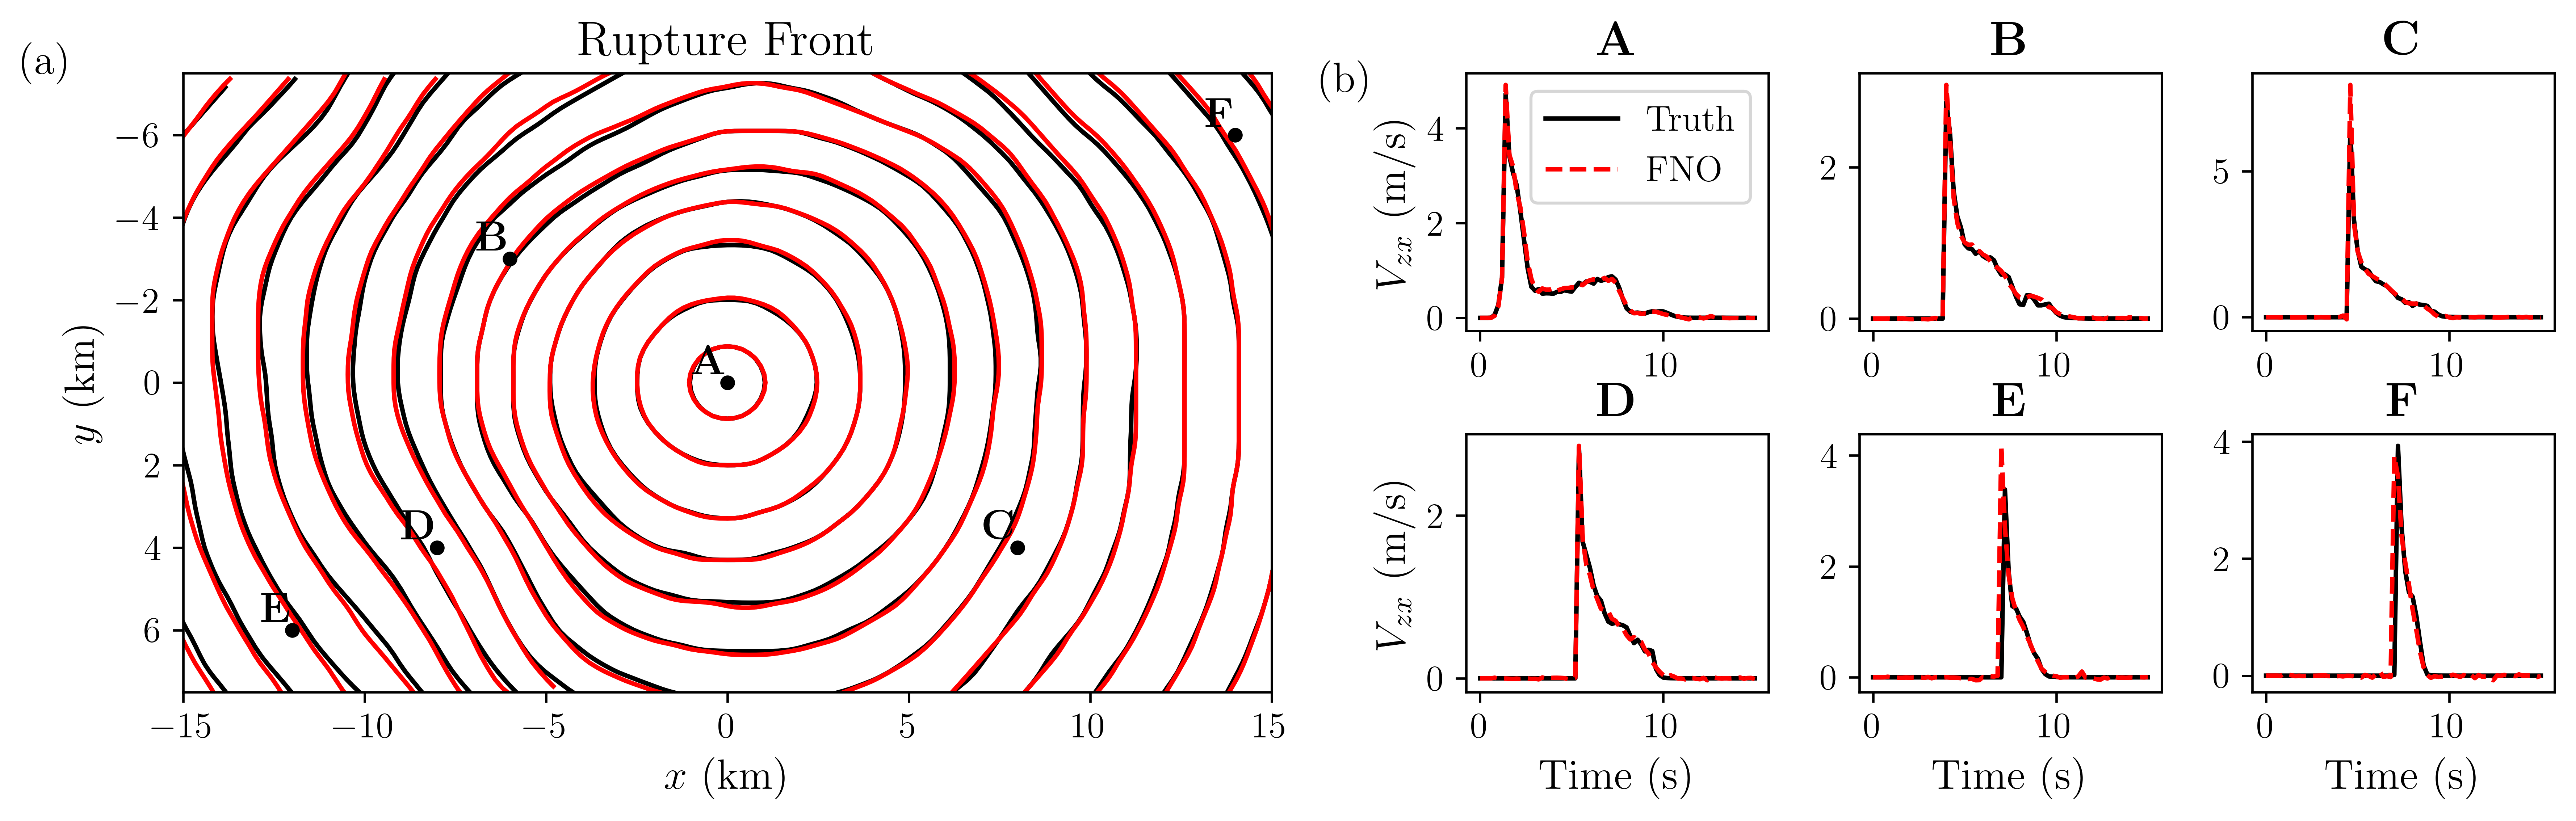
\includegraphics[width=1.0\linewidth]{3D_rupture_front_test2.png}
%DIFDELCMD < %%%
\DIFdelendFL \DIFaddbeginFL 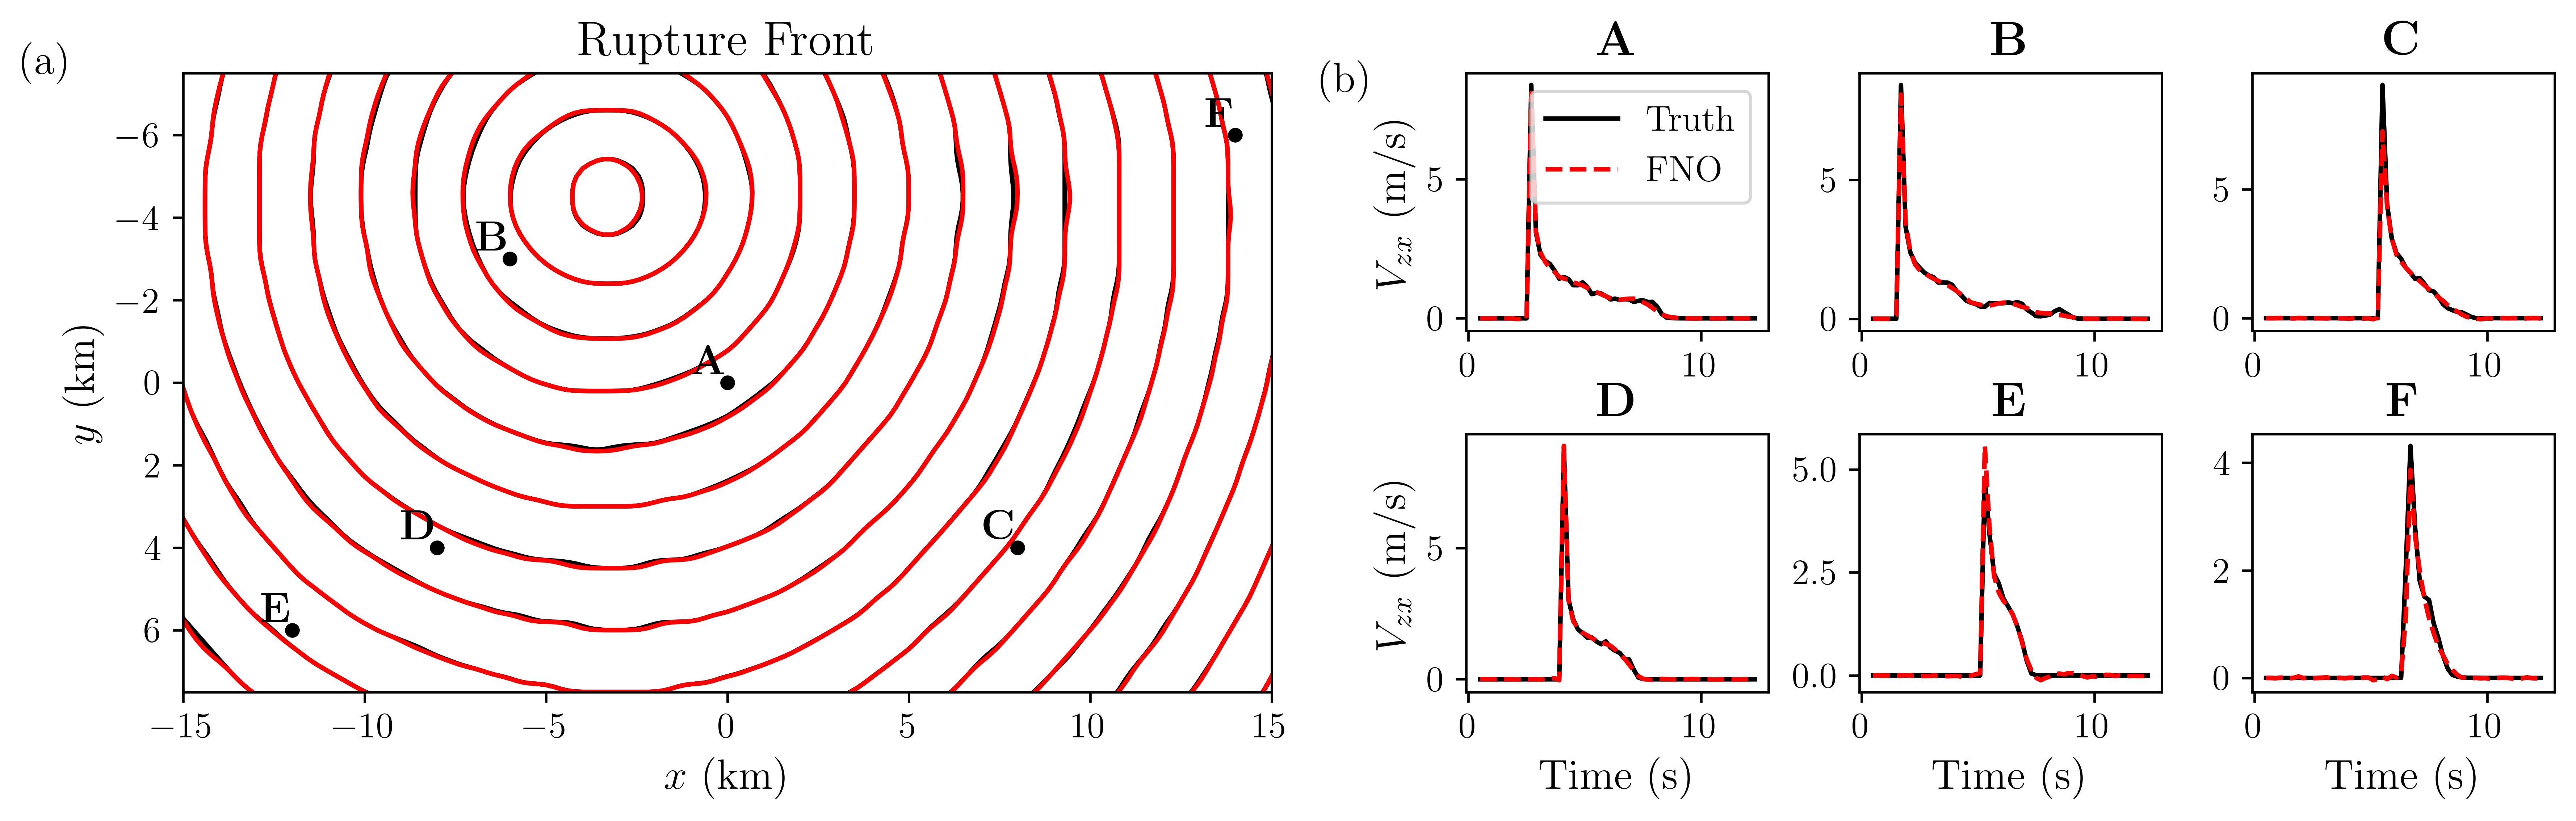
\includegraphics[width=1.0\linewidth]{3D_fractal_test.png}
\DIFaddendFL \caption{\label{fig:3D_test}Results of FNO-2D on the testing dataset for 3D dynamic rupture. \DIFdelbeginFL \DIFdelFL{The inputs }\DIFdelendFL \DIFaddbeginFL \DIFaddFL{Inputs }\DIFaddendFL include \DIFdelbeginFL \DIFdelFL{the initial }\DIFdelendFL \DIFaddbeginFL \DIFaddFL{a }\DIFaddendFL fractal \DIFaddbeginFL \DIFaddFL{initial }\DIFaddendFL shear stress \DIFaddbeginFL \DIFaddFL{distribution }\DIFaddendFL with \DIFdelbeginFL \DIFdelFL{\( D = 1.5 \) }\DIFdelendFL \DIFaddbeginFL \DIFaddFL{\( D = 1.6 \), initial slip rate \( V_{zx0} \) extracted at the threshold \( V_\text{th} = 10^{-3} \) m/s, ten temporal steps of stress perturbation fields, }\DIFaddendFL and \DIFaddbeginFL \DIFaddFL{spatially varying }\DIFaddendFL frictional parameters: \DIFdelbeginFL \DIFdelFL{\( a \) with \( \Delta a_0 = 0.008 \) and \( a_0 = 0.008 \)}\DIFdelendFL \DIFaddbeginFL \DIFaddFL{\( a_0 = 0.007 \)}\DIFaddendFL , \DIFaddbeginFL \DIFaddFL{\( \Delta a_0 = 0.010 \), }\DIFaddendFL and \( b = 0.012 \)\DIFdelbeginFL \DIFdelFL{, over the spatial domain}\DIFdelendFL . (a) \DIFdelbeginFL \DIFdelFL{Rupture }\DIFdelendFL \DIFaddbeginFL \DIFaddFL{Predicted rupture }\DIFaddendFL front \DIFdelbeginFL \DIFdelFL{contour plot, showing progression }\DIFdelendFL \DIFaddbeginFL \DIFaddFL{contours shown }\DIFaddendFL at 0.5 s intervals. (b) Time \DIFdelbeginFL \DIFdelFL{histories }\DIFdelendFL \DIFaddbeginFL \DIFaddFL{series }\DIFaddendFL of slip rate at selected \DIFdelbeginFL \DIFdelFL{points in }\DIFdelendFL \DIFaddbeginFL \DIFaddFL{locations within }\DIFaddendFL the VW region.
}
\end{figure}

 \subsubsection{Generalization to Unseen Initial Shear Stress}
\label{sec:FNO-2D_unseen_shear}

\DIFdelbegin \DIFdel{We }\DIFdelend \DIFaddbegin \DIFadd{Similar to the 2D model, we }\DIFaddend evaluate the trained FNO-2D model using an unseen initial shear stress distribution, specifically \DIFdelbegin \DIFdel{, }\DIFdelend the uniform stress distribution defined in the TPV101 benchmark from the SCEC/USGS dynamic earthquake rupture code verification exercise. In this benchmark, the initial shear stress is uniformly set to 75 MPa, while frictional parameters remain within the training range of the 3D dynamic rupture dataset. 
\DIFaddbegin 

\DIFaddend Figure \ref{fig:3D_SCEC} shows the rupture contours of the predicted component of slip rate \(V_{zx}\) compared to the ground truth, as well as the time history at six selected points in the VW region. FNO-2D can capture the evolution of \(V_{zx}\). The predicted rupture front aligns closely with the ground truth with NRMSE of \DIFdelbegin \DIFdel{0.0100 }\DIFdelend \DIFaddbegin \DIFadd{0.01505 }\DIFaddend and relative \(L_2\) error of \DIFdelbegin \DIFdel{0.2867}\DIFdelend \DIFaddbegin \DIFadd{0.3821}\DIFaddend . The predicted time series also match well with the ground truth, capturing the peaks and fine-scale details of \(V_{zx}\) over time. \DIFdelbegin \DIFdel{The errors in the magnitude of peaks are less than \(1\%\), with some noise observed during the period between the first and second drops at point A. The accuracy drops for points located closer to the VW domain boundaries, with some minor shifts in arrival times and slightly larger mismatch in the peaks (e.g., points E and F). However, overall , there is good agreement between the model predictions and the ground truth}\DIFdelend \DIFaddbegin \DIFadd{Minor time shifts appear at later stages as the rupture approaches the VW boundaries. Although there are some discrepancies in peak magnitudes, which contribute to the overall error, the model successfully captures the rupture arrival time and the overall waveform shape}\DIFaddend . This demonstrates the potential of FNO-2D in capturing the highly nonlinear evolution of slip rate over time, even under an initial shear stress distribution not previously seen during training.

\begin{figure}
\centering
\DIFdelbeginFL %DIFDELCMD < 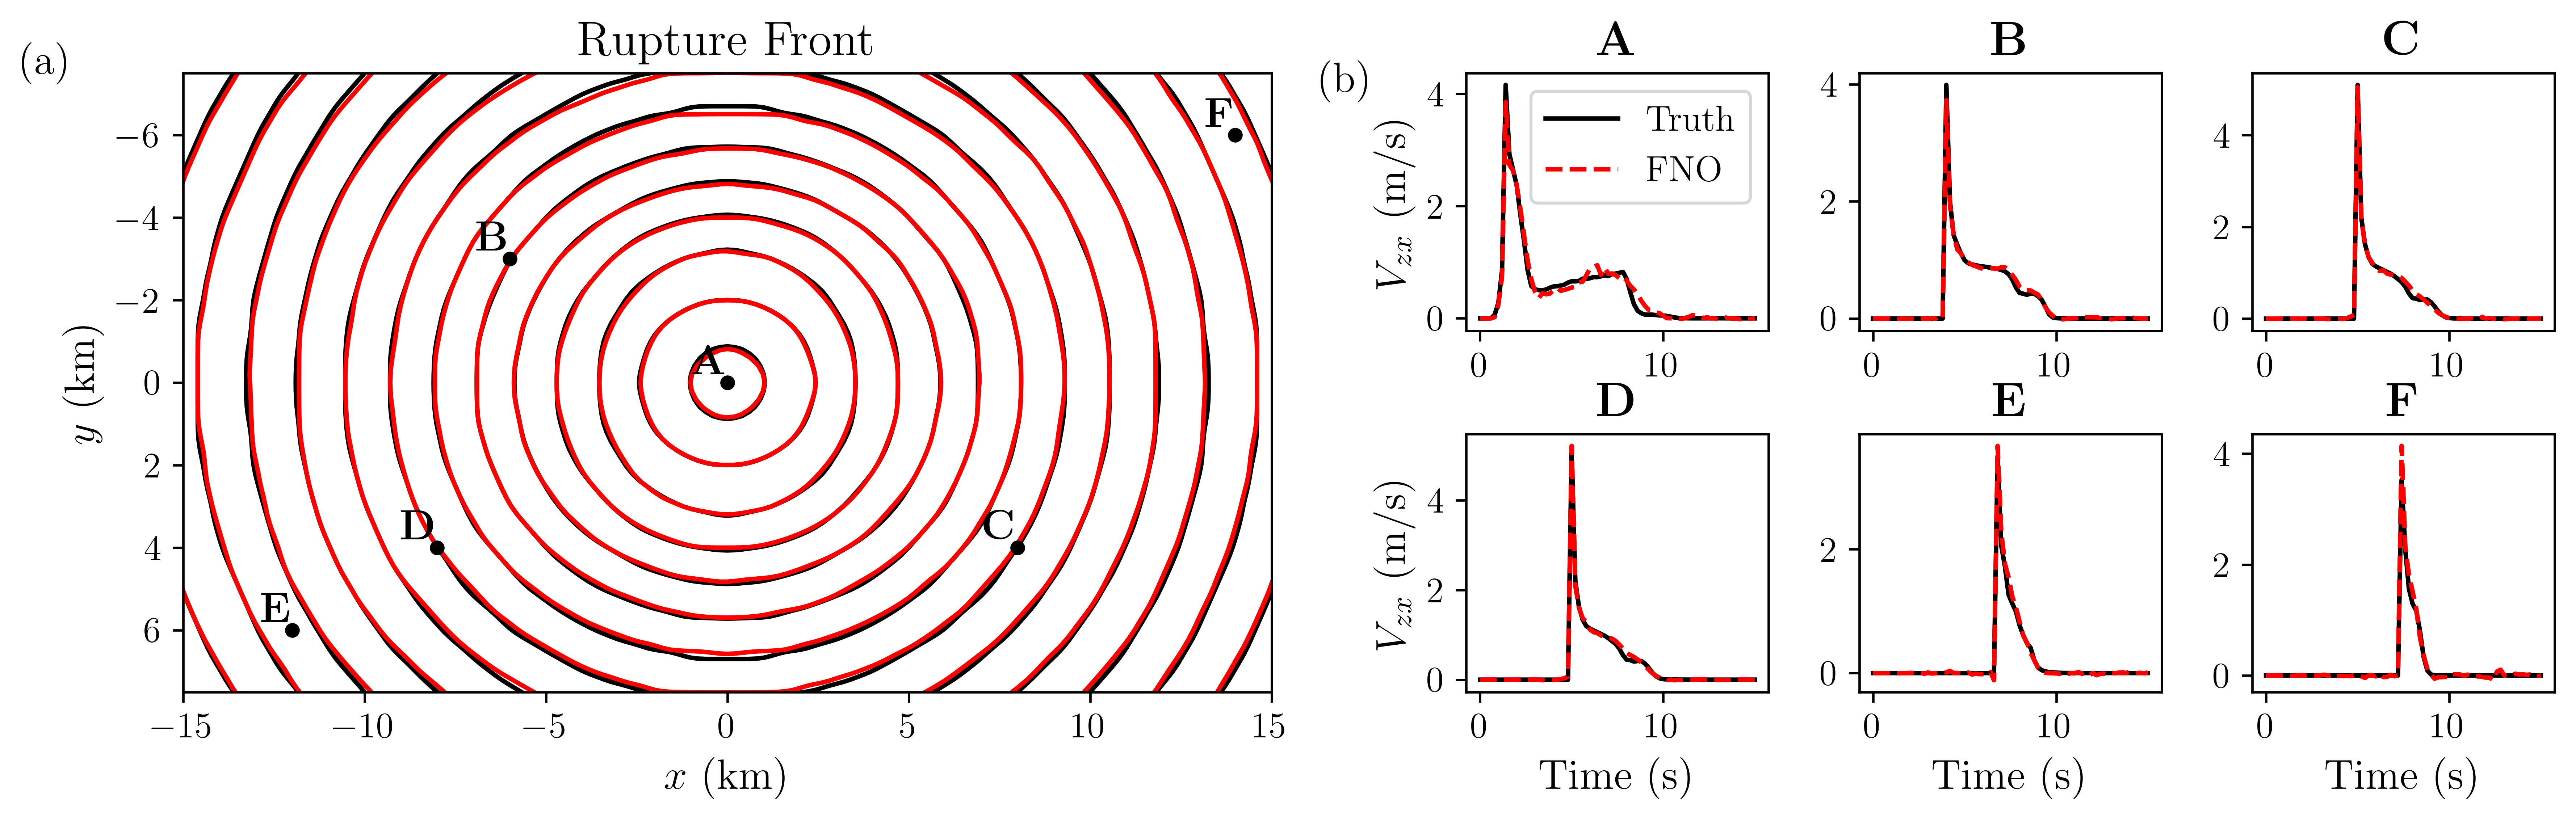
\includegraphics[width=1.0\linewidth]{3D_rupture_front_SCEC2.png}
%DIFDELCMD < %%%
\DIFdelendFL \DIFaddbeginFL 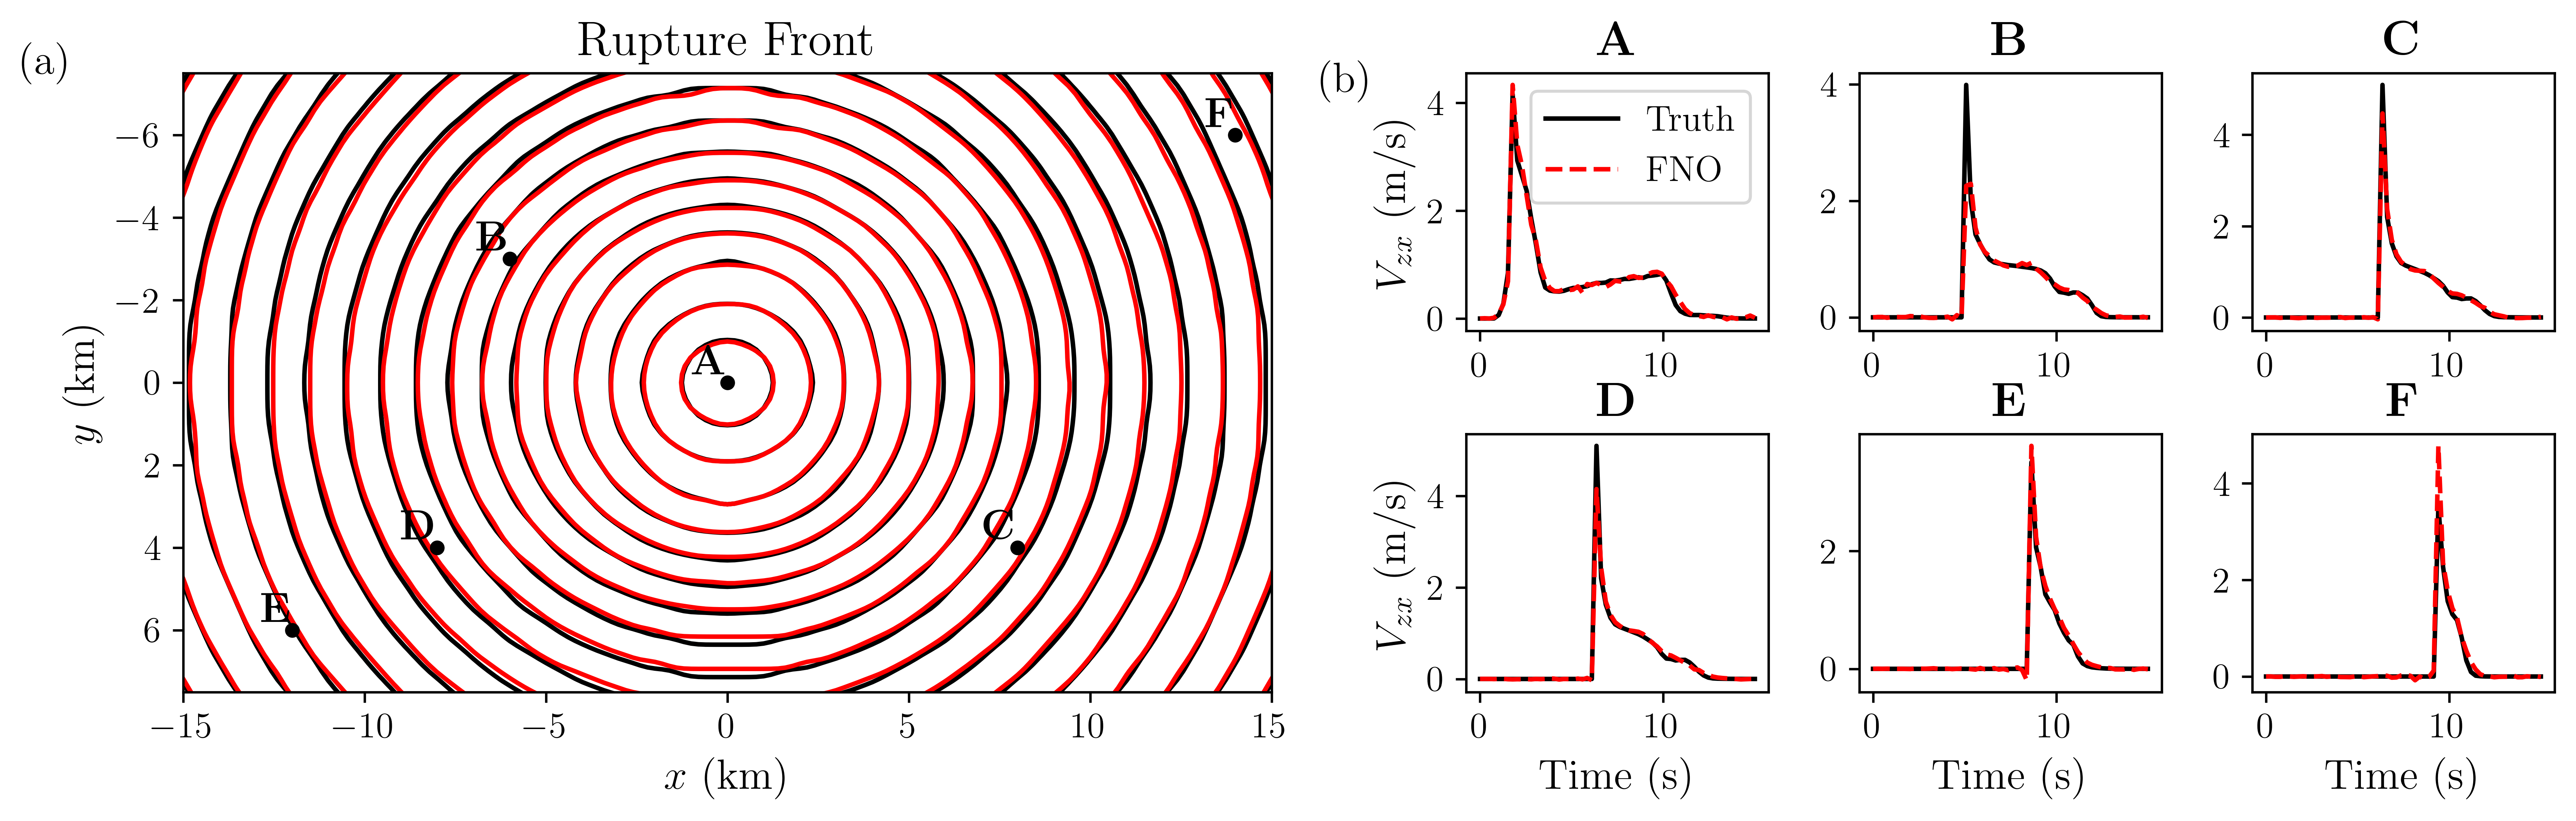
\includegraphics[width=1.0\linewidth]{3D_fractal_unseen_scec.png}
\DIFaddendFL \caption{\label{fig:3D_SCEC}Results of FNO-2D testing on an unseen shear stress distribution from the TPV101 SCEC/USGS benchmark with a uniform shear stress of 75 MPa, \(\Delta a_{0} = 0.008\), \(a_{0} = 0.008\), \DIFdelbeginFL \DIFdelFL{and }\DIFdelendFL \(b = 0.012\)\DIFaddbeginFL \DIFaddFL{, and \(V_\text{th}=0\) m/s}\DIFaddendFL . (a) Rupture front contour plot of the ground truth (black) and predictions (red), showing progression at 0.5 s intervals. (b) Time histories of slip rate at selected points in the VW region.
}
\end{figure}

Additionally, we test the model on a fractal initial shear stress distribution with an unseen fractal dimension \(D = 1.3\), similar to the FNO-1D case. \DIFdelbegin \DIFdel{The frictional parameters are identical to those used previously with FNO-1D.
The predictions , }\DIFdelend \DIFaddbegin \DIFadd{We generate an additional 100 realizations with \(D = 1.3\) and randomly sampled frictional parameters from the seen ranges during training, as listed in Table~\ref{tab:dataset_summary}. We preprocess the data such that \(V_{zx0}\) is chosen at the step following thresholds \(V_\text{th} \in \{0, 10^{-4}, 10^{-3}, 10^{-2}\}\)~m/s. This results in 400 realizations. The distributions of relative \(L_2\) error and NRMSE are shown in Figures \ref{fig:3D_hist_unseen}a and \ref{fig:3D_hist_unseen}c. Both distributions are skewed towards zero, showing generalizability to unseen fractal dimension cases.
}

\begin{figure}
\centering
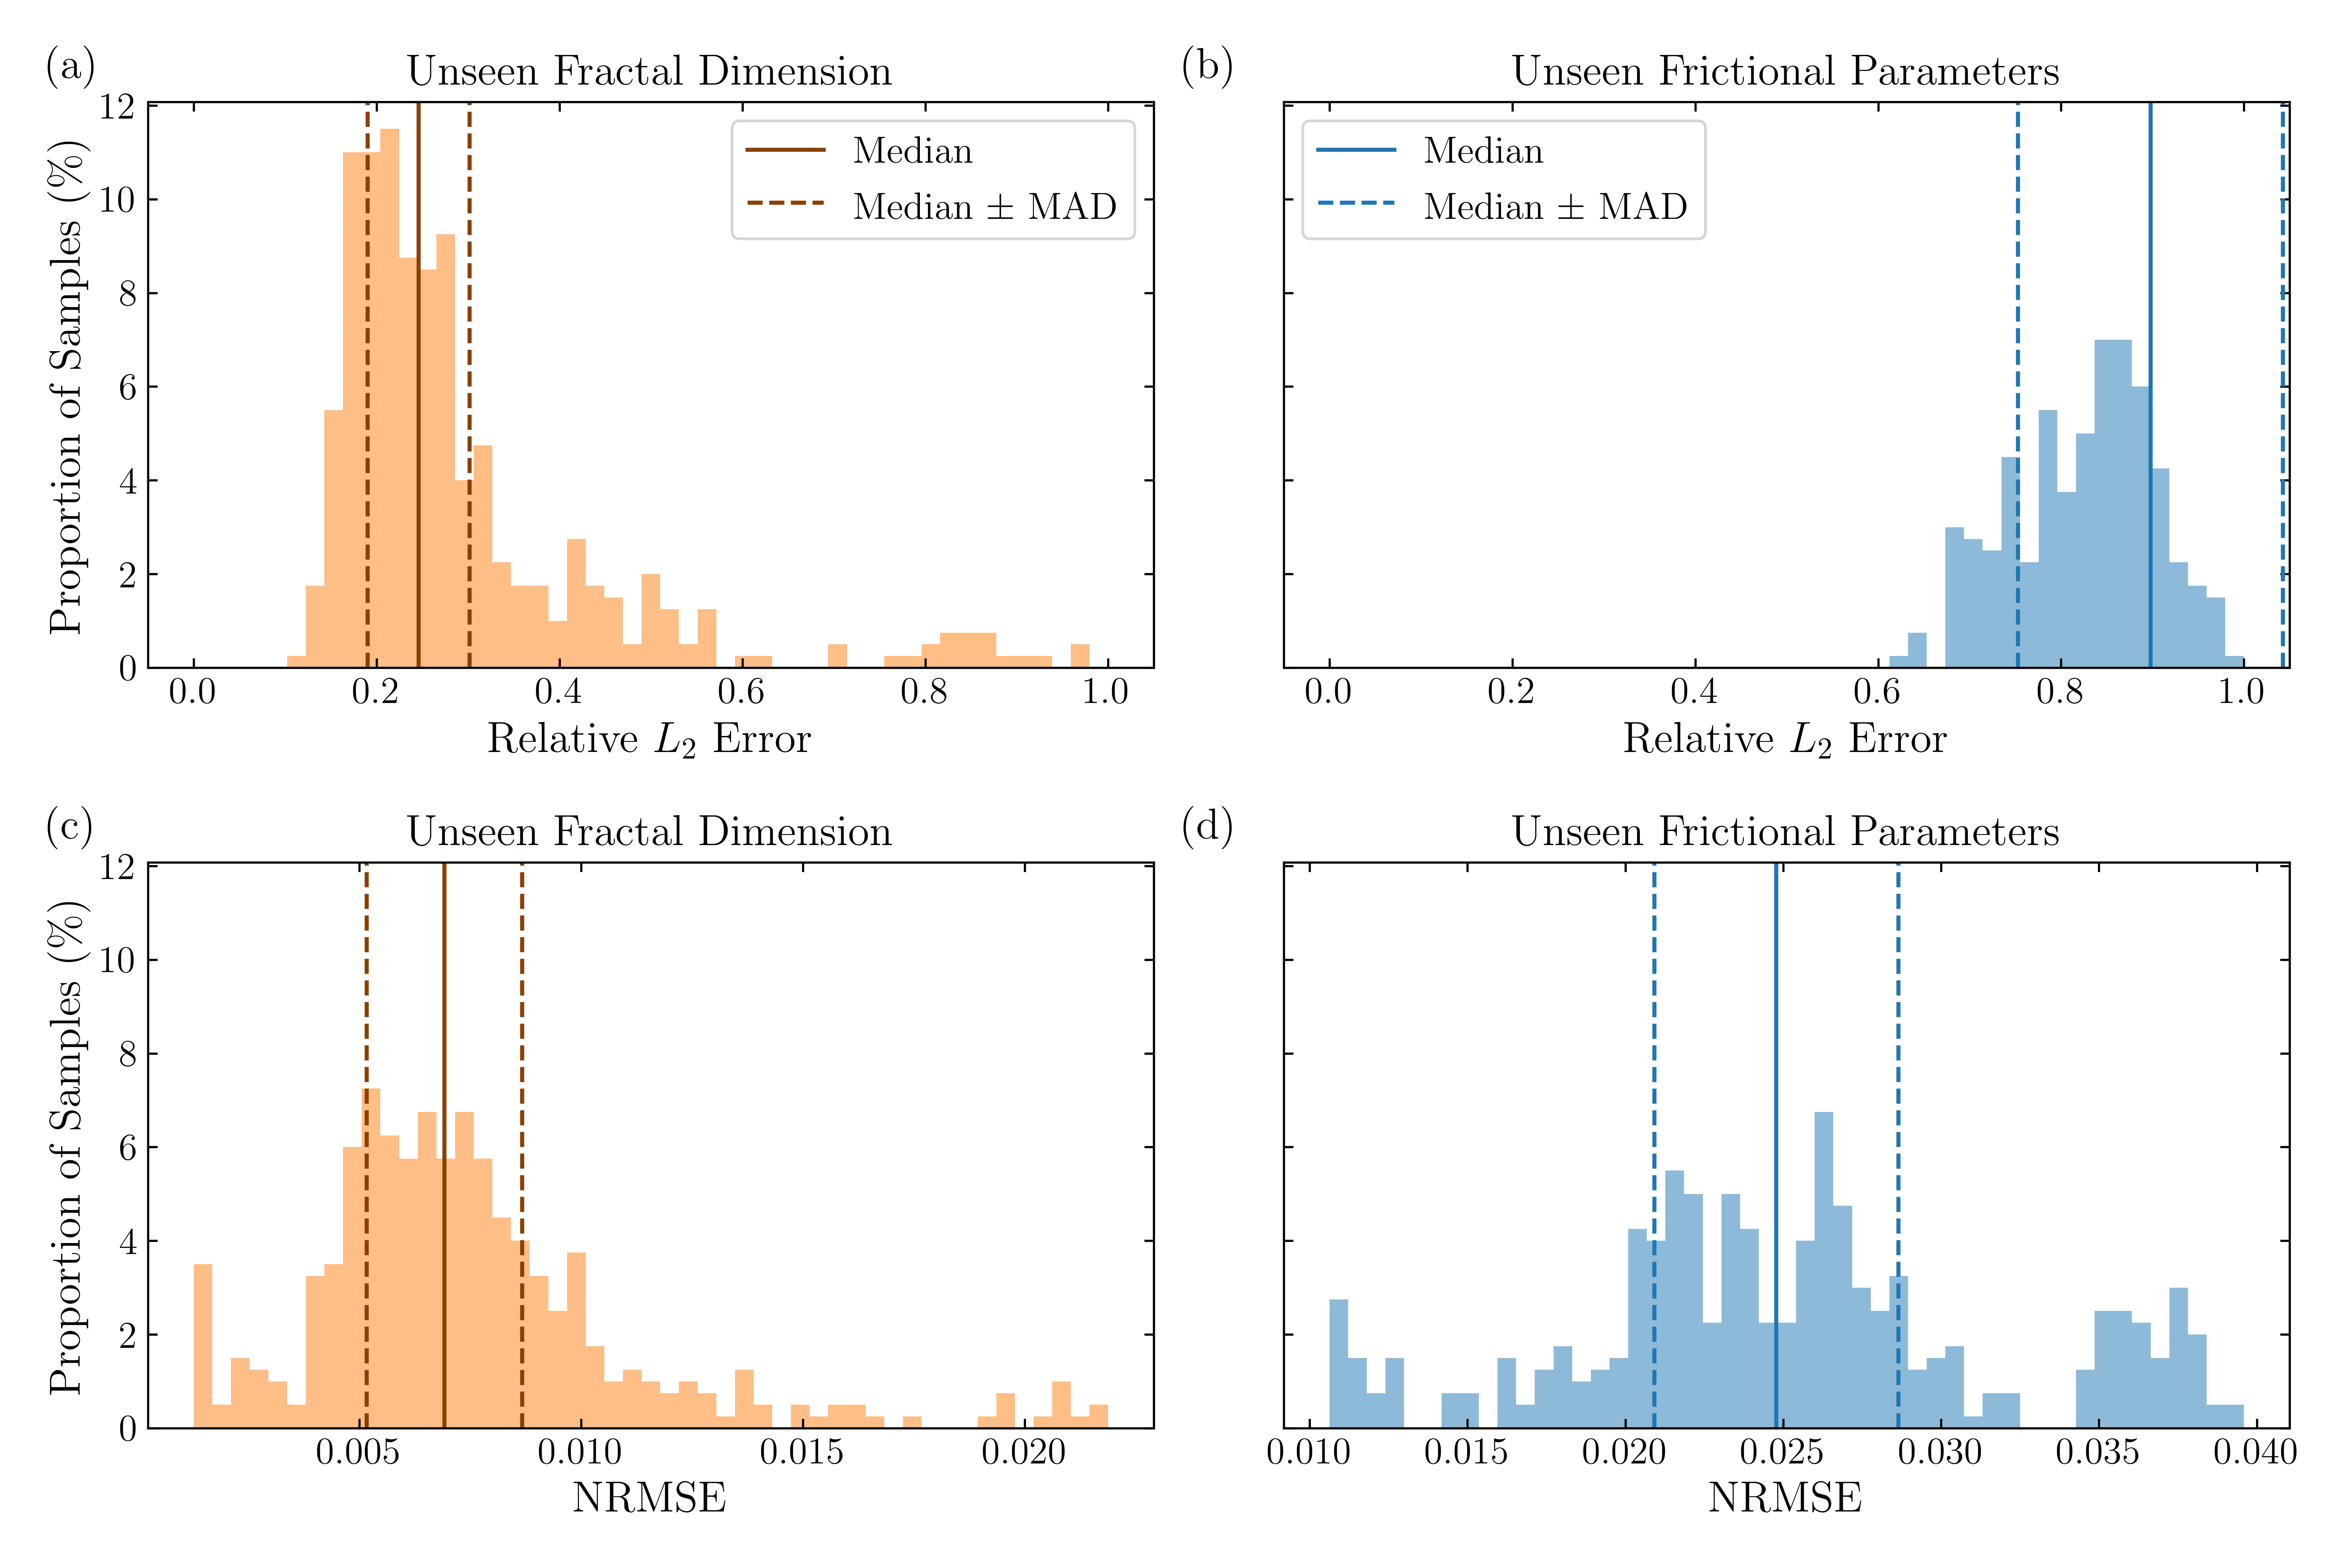
\includegraphics[width=1.0\linewidth]{3D_hist_unseen_2.png}
\caption{\label{fig:3D_hist_unseen}\DIFaddFL{The distribution of (a) the relative \(L_2\) error and (c) the NRMSE evaluated on unseen fractal dimension cases, and (b) the relative \(L_2\) error and (d) the NRMSE evaluated on unseen frictional parameters for the 3D model. These results are based on 400 realizations for each case. Vertical lines indicate the median and MAD. For unseen fractal dimension cases, the median \(\pm\) MAD of the relative error is \(0.245 \pm 0.0557\) and of the NRMSE is \(0.00692 \pm 0.00175\). For unseen frictional parameters cases, the median \(\pm\) MAD of the relative error is \(0.898 \pm 0.145\) and of the NRMSE is \(0.0248 \pm 0.00386\).
}}
\end{figure}


\DIFadd{An example of the predictions is }\DIFaddend presented in terms of the rupture front and time series at selected points in Figure\DIFdelbegin \DIFdel{\ref{fig:3D_fractal_dim13}, show agreement with the ground truth. The shape of the predicted rupture front }\DIFdelend \DIFaddbegin \DIFadd{~\ref{fig:3D_fractal_dim13}. The frictional parameters are \(\Delta a_{0} = 0.011\), \(a_{0} = 0.0065\), and \(b = 0.012\), and here, \(V_\text{th} = 0\)~m/s. The rupture front contour }\DIFaddend aligns with the ground truth\DIFdelbegin \DIFdel{initially, though the match slightly decreases over time, resulting in a NRMSE of 0.00906 }\DIFdelend \DIFaddbegin \DIFadd{, resulting in an NRMSE of 0.00422 }\DIFaddend and a relative \(L_2\) error of \DIFdelbegin \DIFdel{0.3883 }\DIFdelend \DIFaddbegin \DIFadd{0.1284 }\DIFaddend for this realization. \DIFdelbegin \DIFdel{We note that shifts in the rupture front can cause a high relative \(L_2\) error despite the visual agreement. This is due to the small ground truth values, close to zero, being compared to the peak slip rates in the shifted rupture front. The time series at point Eshows slight differences in the peak slip rate. However, it still captures the overall trend of }\DIFdelend \DIFaddbegin \DIFadd{The model accurately captures the rupture arrival time. Peak amplitudes exhibit very small mismatches at points D and E. Furthermore, }\DIFaddend the \DIFdelbegin \DIFdel{evolution}\DIFdelend \DIFaddbegin \DIFadd{predictions of post-peak decay closely match the ground truth}\DIFaddend . This demonstrates that FNO-2D generalizes effectively to different fractal dimensions of \(\tau_{0}\).

\begin{figure}
\centering
\DIFdelbeginFL %DIFDELCMD < 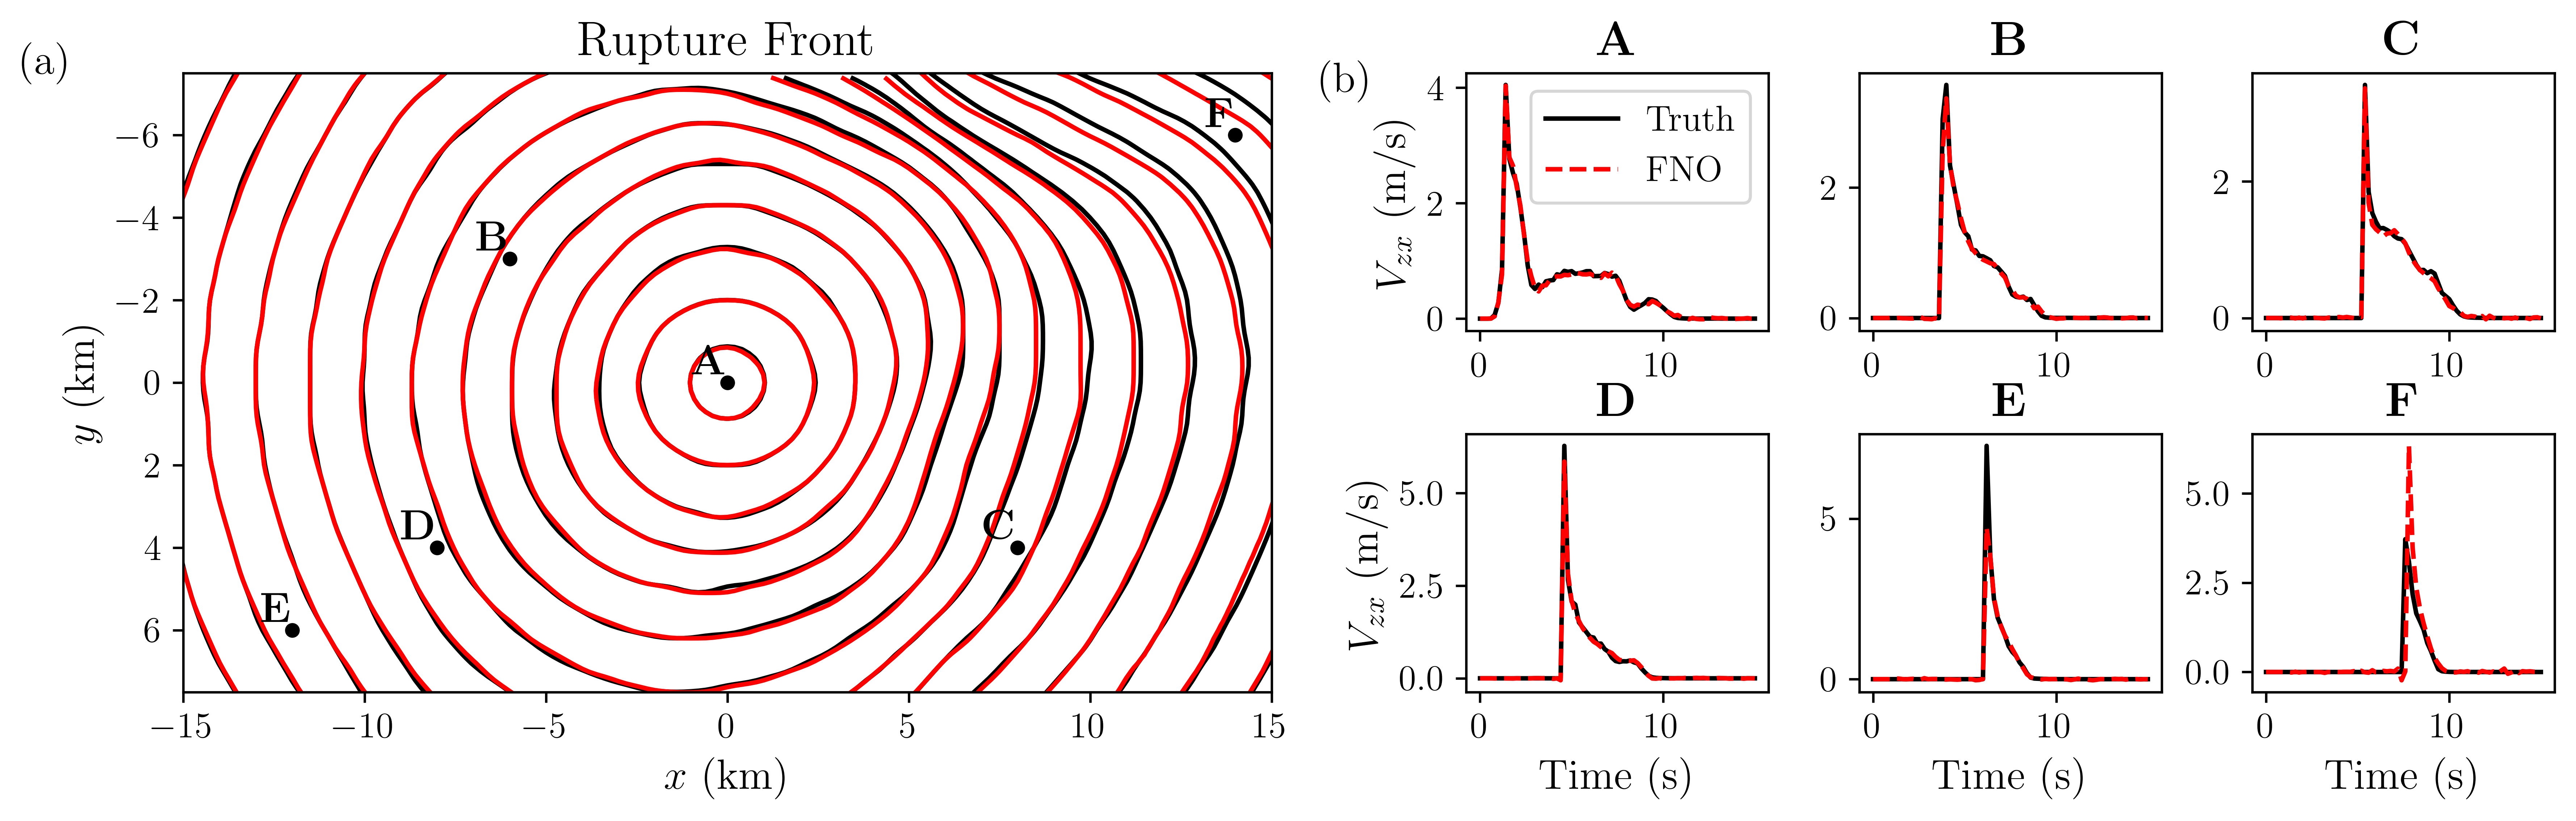
\includegraphics[width=1.0\linewidth]{3D_rupture_front_fractal_dim13_2.png}
%DIFDELCMD < %%%
\DIFdelendFL \DIFaddbeginFL 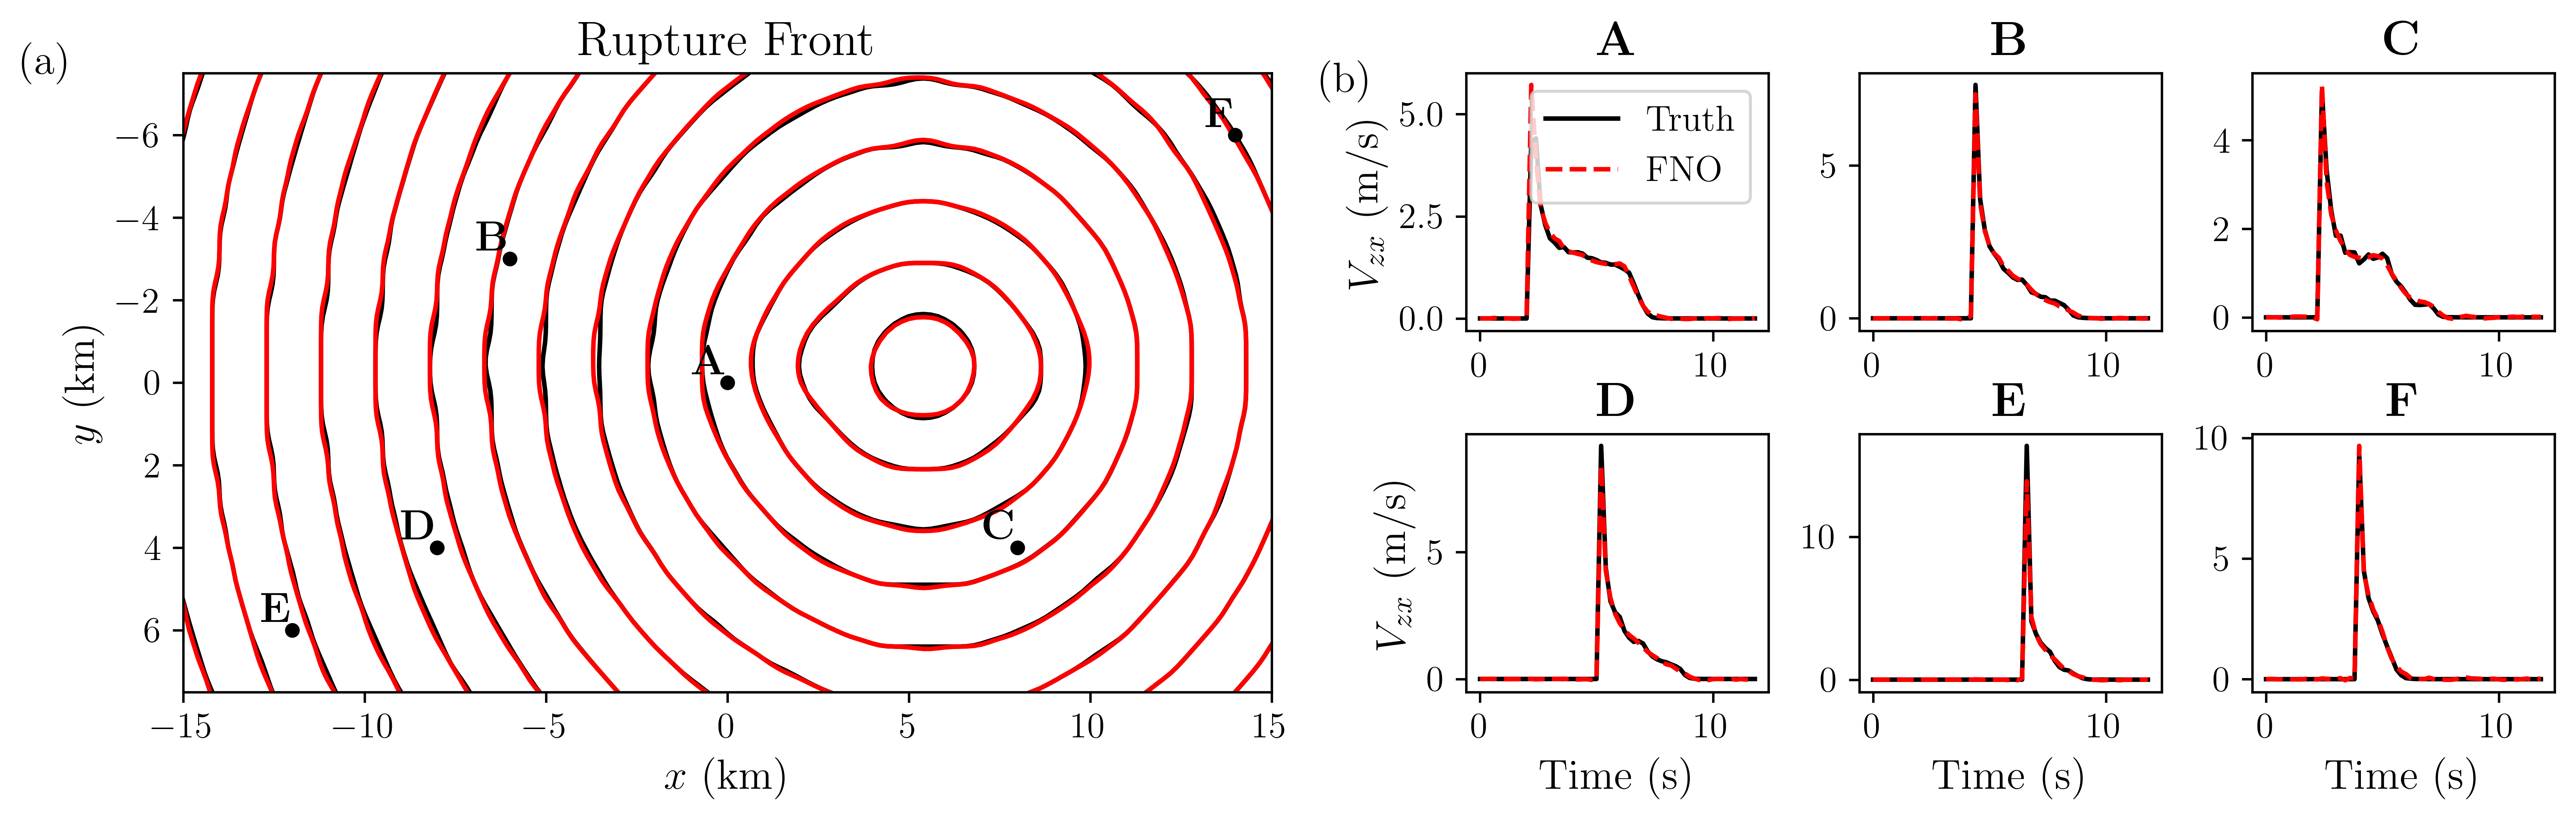
\includegraphics[width=1.0\linewidth]{3D_fractal_unseend.png}
\DIFaddendFL \caption{\label{fig:3D_fractal_dim13}Results of FNO-2D testing on an unseen fractal dimension \(D = 1.3\) of the initial fractal shear stress. The frictional parameters are \DIFdelbeginFL \DIFdelFL{\(\Delta a_{0} = 0.008\)}\DIFdelendFL \DIFaddbeginFL \DIFaddFL{\(\Delta a_{0} = 0.011\)}\DIFaddendFL , \DIFdelbeginFL \DIFdelFL{\(a_{0} = 0.008\)}\DIFdelendFL \DIFaddbeginFL \DIFaddFL{\(a_{0} = 0.0065\)}\DIFaddendFL , and \(b = 0.012\)\DIFaddbeginFL \DIFaddFL{. The initial \(V_{zx0}\) is chosen at the time step where \(V_\text{th}=0\) m/s}\DIFaddendFL : (a) Rupture front contour plot of the ground truth (black) and predictions (red), showing progression at 0.5 s intervals. (b) Time histories of slip rate at selected points in the VW region.
}
\end{figure}

\subsubsection{Generalization to Unseen Frictional Parameters}
\label{sec:FNO-2D_unseen_ab}

We evaluate the generalization performance of the trained FNO-2D model on previously unseen frictional parameter values. Specifically, \DIFdelbegin \DIFdel{parameter \(a\) }\DIFdelend \DIFaddbegin \DIFadd{we generate 100 realizations using frictional parameters sampled from combinations not included in the training dataset, as summarized in Table~\ref{tab:dataset_summary_unseenab}. After preprocessing the data based on velocity thresholds \( V_{\text{th}} \in \{0, 10^{-4}, 10^{-3}, 10^{-2}\} \), we obtain a total of 400 realizations with varying \( V_{zx0} \) fields. Figures \ref{fig:3D_hist_unseen}b and \ref{fig:3D_hist_unseen}d show the distributions of the relative \(L_2\) error and the NRMSE, respectively. Although the relative \(L_2\) error is high, with a median of \(0.898\), the range of the NRMSE in the 3D model is smaller than that in the 2D model. Despite the lower accuracy as measured by the relative \(L_2\) error, the 3D model demonstrates greater stability in terms of normalized error when compared with the observed range in \(V_{zx}\).
}


\DIFadd{Figure~\ref{fig:3D_unseen_ab} illustrates a representative case, including the predicted rupture front and time histories of the slip rate component \( V_{zx} \) at selected spatial locations. In this example, the frictional parameter \( a \) }\DIFaddend is set to \DIFdelbegin \DIFdel{\(0.0075\) }\DIFdelend \DIFaddbegin \DIFadd{\( 0.0067 \) }\DIFaddend in the VW region and \DIFdelbegin \DIFdel{\(0.0165\) }\DIFdelend \DIFaddbegin \DIFadd{\( 0.0177 \) }\DIFaddend in the VS region, while parameter \DIFdelbegin \DIFdel{\(b\) }\DIFdelend \DIFaddbegin \DIFadd{\( b \) }\DIFaddend is uniformly fixed at \DIFdelbegin \DIFdel{\(0.012\) }\DIFdelend \DIFaddbegin \DIFadd{\( 0.012 \) }\DIFaddend along the fault. The initial shear stress \DIFdelbegin \DIFdel{\(\tau_{0}\) is modeled }\DIFdelend \DIFaddbegin \DIFadd{\( \tau_{0} \) is constructed }\DIFaddend using a fractal distribution with \DIFdelbegin \DIFdel{fractal dimension \(D = 1.5\).
Figure \ref{fig:3D_unseen_ab} presents a successful case of the predicted rupture front and corresponding time series of \(V_{zx}\) at selected spatial locations. }\DIFdelend \DIFaddbegin \DIFadd{a fractal dimension \( D = 1.5 \).
}

\DIFaddend We observe spatial \DIFdelbegin \DIFdel{shifts }\DIFdelend \DIFaddbegin \DIFadd{and temporal discrepancies }\DIFaddend in the rupture front contours \DIFdelbegin \DIFdel{, which amplify the NMRSE and relative \(L_2\) error to 0.0171 and 0.6051, respectively. Some mismatches at the peaks of \(V_{zx}\) over time at selected points also contribute to this error. While }\DIFdelend \DIFaddbegin \DIFadd{and the time histories at points C, E, and F, which contribute to elevated errors, with an NRMSE of 0.0219 and a relative \( L_2 \) error of 0.6767. In particular, mismatches in the peak magnitudes of \( V_{zx} \) at these locations account for a significant portion of the error. However, }\DIFaddend the FNO-2D \DIFdelbegin \DIFdel{still captures the global features of the }\DIFdelend \DIFaddbegin \DIFadd{model successfully captures the overall }\DIFaddend temporal evolution of \DIFdelbegin \DIFdel{\(V_{zx}\) across }\DIFdelend \DIFaddbegin \DIFadd{\( V_{zx} \), including the }\DIFaddend nucleation, propagation, and arrest phases \DIFdelbegin \DIFdel{, we later discuss specific challenges related to }\DIFdelend \DIFaddbegin \DIFadd{of rupture. In the following discussion, we address the specific challenges in }\DIFaddend generalizing to unseen frictional properties and \DIFdelbegin \DIFdel{how to possibly improve the relative \(L_2\) error}\DIFdelend \DIFaddbegin \DIFadd{propose strategies to improve predictive accuracy}\DIFaddend .

\begin{figure}
\centering
\DIFdelbeginFL %DIFDELCMD < 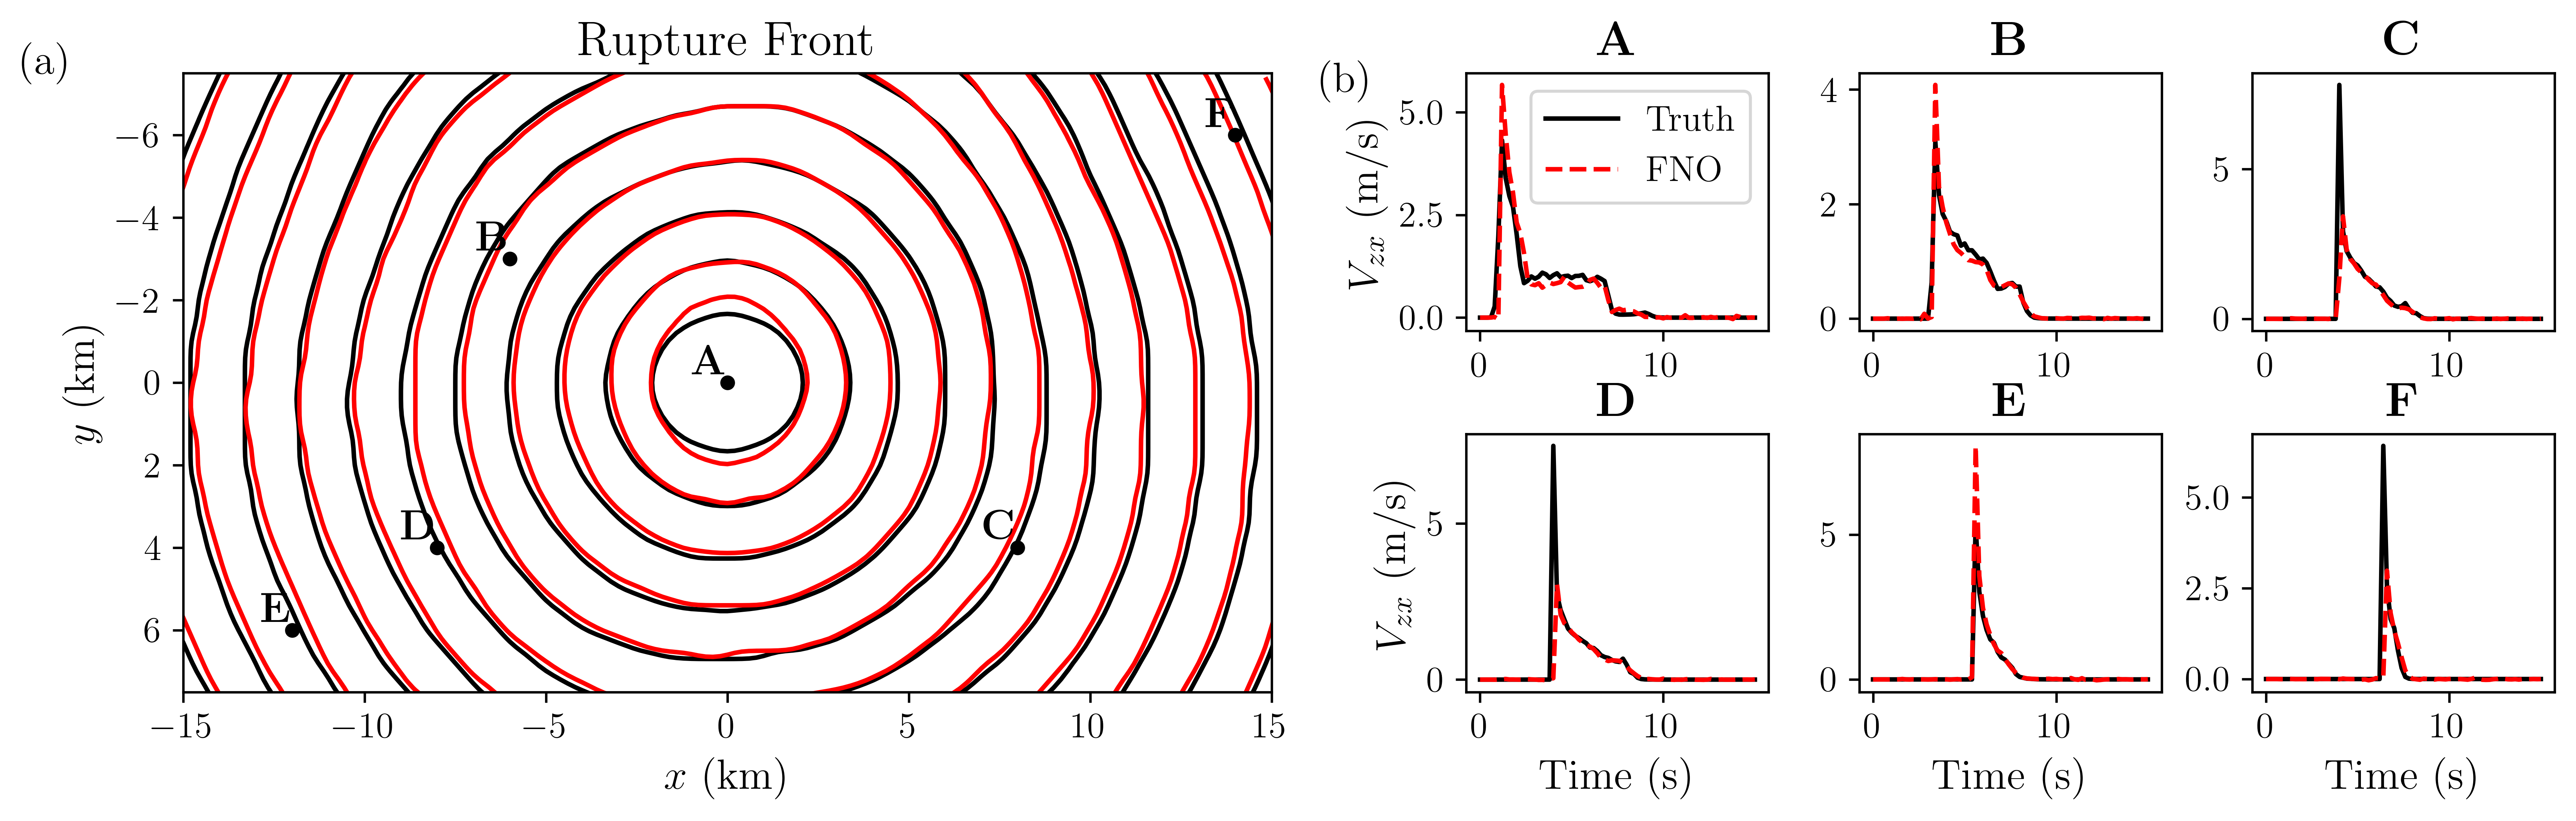
\includegraphics[width=1.0\linewidth]{3D_rupture_front_ab009_2.png}
%DIFDELCMD < %%%
\DIFdelendFL \DIFaddbeginFL 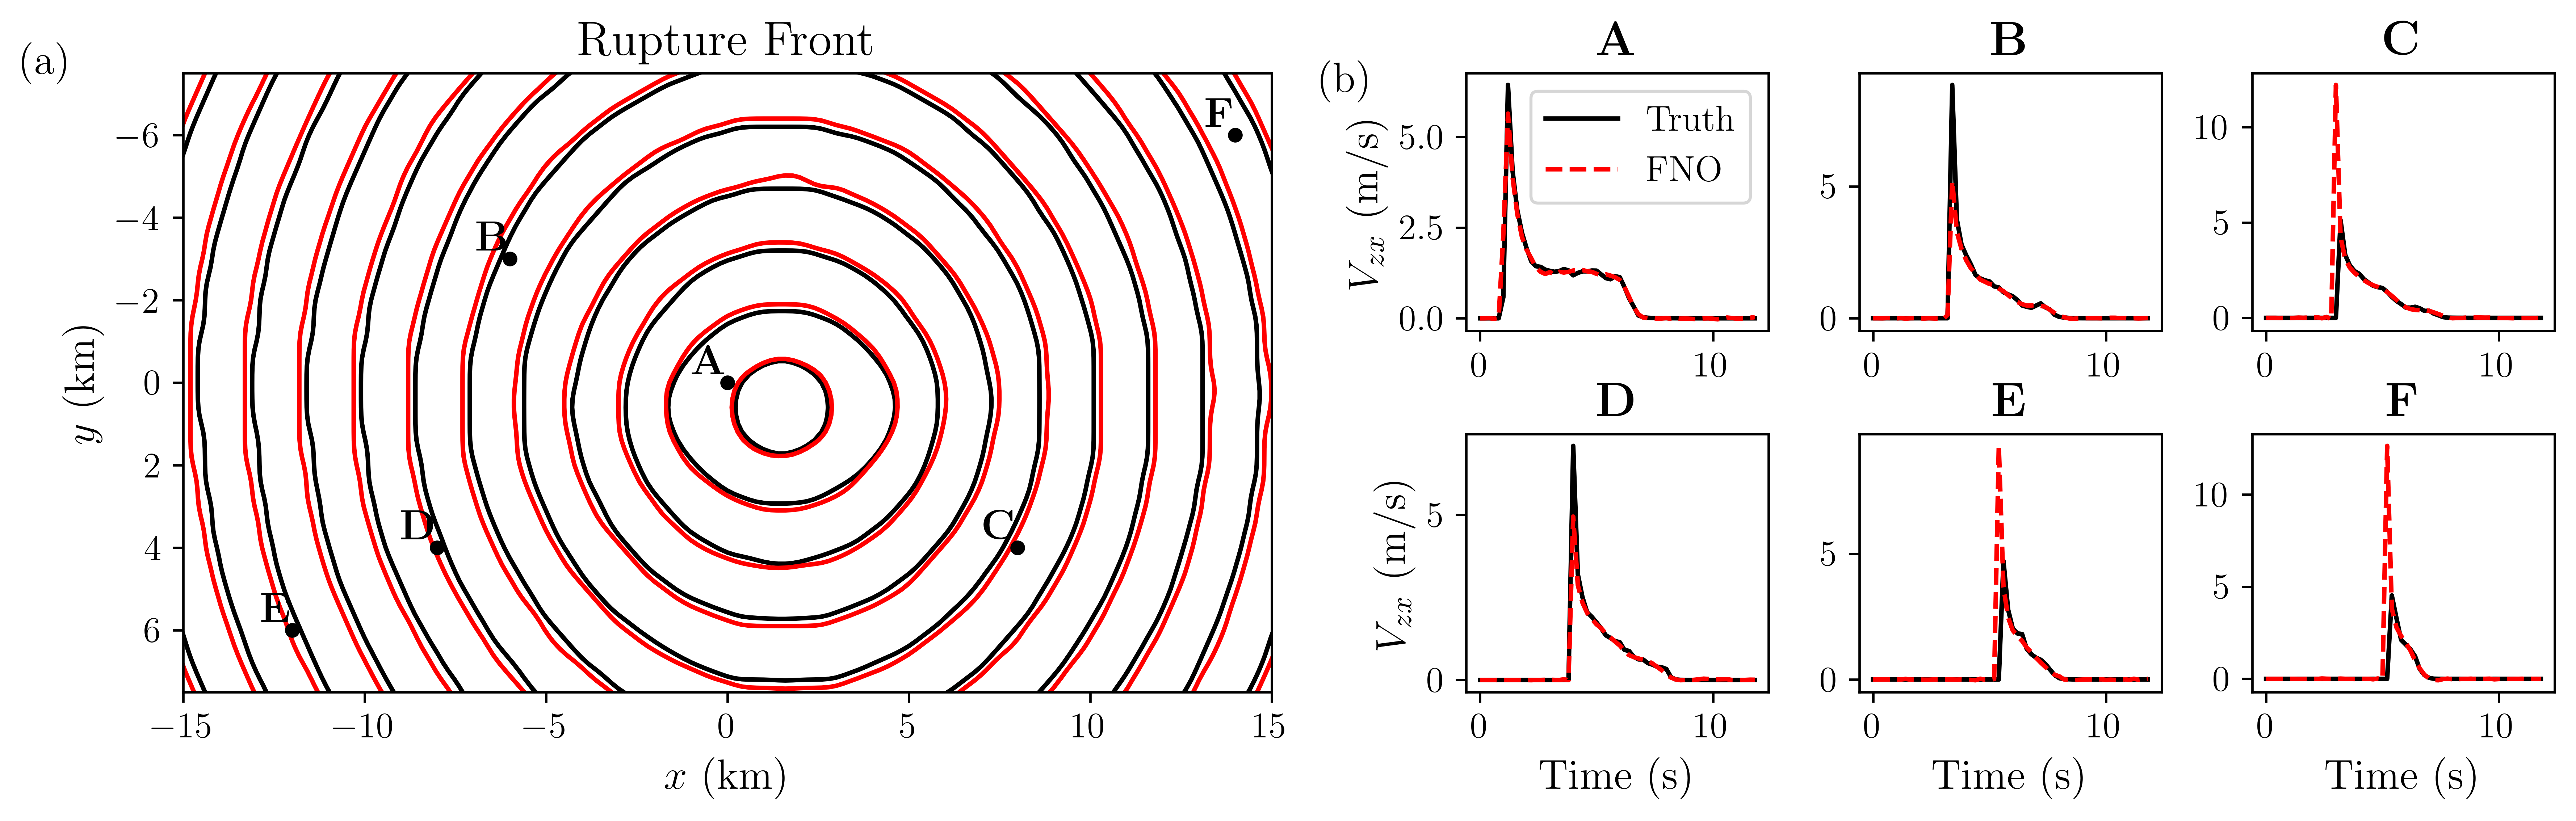
\includegraphics[width=1.0\linewidth]{3D_fractal_unseenab.png}
\DIFaddendFL \caption{\label{fig:3D_unseen_ab}Results of FNO-2D testing on an unseen \(a-b\) distribution. Inputs consist of frictional parameters \(a\) and \(b\), with \DIFdelbeginFL \DIFdelFL{\(\Delta a_{0} = 0.009\)}\DIFdelendFL \DIFaddbeginFL \DIFaddFL{\(\Delta a_{0} = 0.011\)}\DIFaddendFL , \DIFdelbeginFL \DIFdelFL{\(a_{0} = 0.0075\)}\DIFdelendFL \DIFaddbeginFL \DIFaddFL{\(a_{0} = 0.0067\)}\DIFaddendFL , and \(b = 0.012\), along with an initial shear stress distribution \(\tau_{0}\) with a fractal dimension \(D = 1.5\) \DIFaddbeginFL \DIFaddFL{and \(V_\text{th}=0\) m/s}\DIFaddendFL . (a) Rupture front contour plot showing progression at 0.5 s intervals. (b) Time histories of slip rate at selected points in the VW region.
}
\end{figure}

\subsection{Computational Efficiency Analysis}
\label{sec:comp_efficienvy}

We summarize the computational efficiency of FNO-1D and FNO-2D in Table \ref{tab:model_comparison}. \DIFdelbegin \DIFdel{The training }\DIFdelend \DIFaddbegin \DIFadd{Training }\DIFaddend and testing times are \DIFdelbegin \DIFdel{both evaluated on an Nvidia }\DIFdelend \DIFaddbegin \DIFadd{reported for an NVIDIA }\DIFaddend A100 GPU\DIFdelbegin \DIFdel{. Once the models are trained , they }\DIFdelend \DIFaddbegin \DIFadd{, while the 3D dynamic rupture dataset is trained using four parallel NVIDIA A100 GPUs. Once trained on the NCSA Delta system via ACCESS allocation \mbox{%DIFAUXCMD
\cite{boerner2023access}}\hskip0pt%DIFAUXCMD
, these models }\DIFaddend can be directly \DIFdelbegin \DIFdel{used as an alternative }\DIFdelend \DIFaddbegin \DIFadd{employed as efficient alternatives }\DIFaddend to numerical simulators.

For the application we are proposing, the trained model is used directly for subsequent predictions. Therefore, we compare the FNO model's performance to the computational time required by a numerical solver. To evaluate the \DIFaddbegin \DIFadd{potential }\DIFaddend computational speed-up, we compare the numerical simulation run time on an AMD EPYC 7763 “Milan” (PCIe Gen4) CPU to the FNO's testing time. The run times are 345 s for the 2D simulation and 1182 s for the 3D simulation. The predictions from the 2D and 3D simulations are $2 \times 10^{5}$ and $4 \times 10^{5}$ times faster than the conventional numerical simulation, respectively.

Notably, the prediction time does not increase significantly, despite the substantial increase in the number of parameters, from 2D to 3D. The training time is slower for the 3D simulation. However, we prioritize prediction accuracy and testing time over the off-line training time.

\begin{table}
\caption{Comparison of different models in terms of parameters, training time, testing performance, and speed-up. The testing times are calculated by taking the median of 100 random cases. The speed-up is compared with numerical simulation run time of 345 s for 2D and 1182 s for 3D.}
    \centering
    \DIFdelbeginFL %DIFDELCMD < \resizebox{\textwidth}{!}{ % Resize table to fit within text width
%DIFDELCMD <     \begin{tabular}{lcccc}
%DIFDELCMD <         \toprule
%DIFDELCMD <         & \# Parameter & Training & \multicolumn{2}{c}{Testing} \\
%DIFDELCMD <         \cmidrule(lr){4-5}
%DIFDELCMD <         & (–) & (s/epoch) & Prediction time (s) & Speed-up vs. numerical simulation (times) \\
%DIFDELCMD <         \midrule
%DIFDELCMD <         FNO-1D & 2,348,492 & 3  & 0.002 & $2 \times 10^5$ \\
%DIFDELCMD <         FNO-2D & 268,739,404 & 130  & 0.003 & $4 \times 10^5$ \\
%DIFDELCMD <         \bottomrule
%DIFDELCMD <     \end{tabular}
%DIFDELCMD <     }
%DIFDELCMD <     %%%
\DIFdelendFL \DIFaddbeginFL \resizebox{\textwidth}{!}{ % Resize table to fit within text width
    \begin{tabular}{lcccc}
        \toprule
        & \# Parameter & Training & \multicolumn{2}{c}{Testing} \\
        \cmidrule(lr){4-5}
        & (–) & (s/epoch) & Prediction time (s) & Speed-up vs. numerical simulation (times) \\
        \midrule
        FNO-1D & 2,348,492 & 30  & 0.002 & $2 \times 10^5$ \\
        FNO-2D & 268,739,404 & 594  & 0.003 & $4 \times 10^5$ \\
        \bottomrule
    \end{tabular}
    }
    \DIFaddendFL \label{tab:model_comparison}
\end{table}


\section{Discussion and Conclusion}
\label{sec:discussion}

To overcome the computational bottleneck of classical physics-based earthquake models, we present an FNO-based surrogate model to accelerate dynamic rupture simulations. In the surrogate model, we predict the evolution of the slip rate distribution on the fault plane, given the initial distribution of shear stress\DIFaddbegin \DIFadd{, slip rate, stress perturbation, }\DIFaddend and frictional parameters \(a\) and \(b\) in the rate-and-state friction law\DIFdelbegin \DIFdel{, a commonly used friction law in earthquake modeling}\DIFdelend . The ground truth is generated using the SBI method with different \DIFaddbegin \DIFadd{initial }\DIFaddend fractal shear stress\DIFaddbegin \DIFadd{, slip rate, nucleation site, }\DIFaddend and frictional parameter distributions in both 2D and 3D \DIFdelbegin \DIFdel{homogeneous }\DIFdelend domains. Each dataset is trained and tuned separately using FNO-1D and FNO-2D. We select the hyperparameters based on a balance between computational efficiency and accuracy as discussed in \DIFdelbegin \DIFdel{Appendix }\DIFdelend \ref{sec:appendix_b}. As a result, we achieve speedups of \( 4 \times 10^5 \) and \( 2 \times 10^5 \) compared to the SBI method in 3D and 2D dynamic rupture problems, respectively. This increase in speed potentially enables more efficient dynamic rupture inversion, statistical analysis, and identification of extreme events in ensembles of earthquake rupture forecasts.

Predicted slip rates are evaluated using pointwise metrics, including the \DIFdelbegin \DIFdel{normalized root mean squared error (NRMSE)}\DIFdelend \DIFaddbegin \DIFadd{NRMSE}\DIFaddend , which compares predictions with the observed range of the ground truth, and the relative \(L_2\) error, which assesses the discrepancy at discrete points in the domain. We demonstrate that the training process of FNO-based models does not exhibit overfitting. Test set predictions show strong agreement with the ground truth. Specifically, for the 2D dynamic rupture dataset, the median NRMSE is \DIFdelbegin \DIFdel{\(0.329\%\) }\DIFdelend \DIFaddbegin \DIFadd{\(0.388\%\) }\DIFaddend and the median relative \(L_2\) error is \DIFdelbegin \DIFdel{\(6.85\%\)}\DIFdelend \DIFaddbegin \DIFadd{\(2.70\%\)}\DIFaddend . For the 3D dynamic rupture dataset, the median NRMSE is \DIFdelbegin \DIFdel{\(0.387\%\) }\DIFdelend \DIFaddbegin \DIFadd{\(0.366\%\) }\DIFaddend and the median relative \(L_2\) error is \DIFdelbegin \DIFdel{\(15.3\%\)}\DIFdelend \DIFaddbegin \DIFadd{\(13.3\%\)}\DIFaddend . 

Higher errors in the 3D problem are primarily due to down-sampling to a lower resolution than the physical problem, resulting in a grid size that may smear some details in the process zone region. This limitation is due to constrained computational resources. Access to additional resources would allow training at higher resolution, potentially reducing these errors to a level comparable to what is seen in the 2D problem. The errors are generally more pronounced in regions with high-frequency features, reflecting the spectral bias, which states that deep learning models tend to favor low-frequency components. To further improve model performance, we suggest training on a \DIFdelbegin \DIFdel{specialized dataset, with the most critical hyperparameter being the width of \(P\) and \(Q\).   
This opens opportunities for further improving the model performance by increasing the size of the training dataset as well as increasing the model complexity.  
}\DIFdelend \DIFaddbegin \DIFadd{larger dataset.   
}\DIFaddend 

\DIFdelbegin \DIFdel{Furthermore, we test the model }\DIFdelend \DIFaddbegin \DIFadd{We also evaluate the models }\DIFaddend under unseen initial stress distributions and frictional parameters. The FNO-based models \DIFdelbegin \DIFdel{demonstrate robustness when applied to }\DIFdelend \DIFaddbegin \DIFadd{show robustness in }\DIFaddend out-of-distribution cases, such as a uniform initial stress distribution \DIFdelbegin \DIFdel{. Under this distribution, the problem setup corresponds }\DIFdelend \DIFaddbegin \DIFadd{corresponding }\DIFaddend to the SCEC/USGS verification exercise. \DIFdelbegin \DIFdel{Additionally, we evaluate the model on an initial }\DIFdelend \DIFaddbegin \DIFadd{They also perform well on a }\DIFaddend shear stress distribution with an unseen fractal dimension of \DIFdelbegin \DIFdel{\(D=1.3\). The FNO-based models maintain good accuracy under these conditions, with NRMSE values lower than \(1 \%\). We also test FNO-1D and FNO-2D }\DIFdelend \DIFaddbegin \DIFadd{\(D = 1.3\), achieving median relative \(L_2\) errors of 31.3\% in 2D and 24.5\% in 3D. By contrast, when tested }\DIFaddend on unseen frictional parameters\DIFdelbegin \DIFdel{. While we have demonstrated successful predictions for unseen frictional parameters}\DIFdelend , the model \DIFdelbegin \DIFdel{'s performance is less robust compared to tests involving unseen shear stress}\DIFdelend \DIFaddbegin \DIFadd{yields a median relative \(L_2\) error of 13.0\% in 2D but 89.8\% in 3D. One important source of error in FNO predictions is spatial and temporal shifts. When the slip rate is small, the relative \(L_2\) error can be amplified, particularly where sharp, high-value rupture fronts shift in space and time relative to small slip rate values}\DIFaddend . This reduced robustness may be attributed to the fact that variations in frictional parameters modify the underlying material model and consequently change the properties of the governing operator. In contrast, changing the shear stress distribution affects only the initial conditions without modifying the governing equations. This limitation could \DIFdelbegin \DIFdel{potentially be addressed by incorporating a greater variety of frictional parameters during training }\DIFdelend \DIFaddbegin \DIFadd{be mitigated by training with a larger datasets. As demonstrated in Section~\ref{sec:appendix_b}, increasing the size of the training dataset improves performance. A shared community database of large-scale dynamic rupture simulations would be highly beneficial}\DIFaddend .
\DIFdelbegin \DIFdel{One important source of error in FNO predictions is spatial and temporal shifts. When the slip rate is small, the relative \(L_2\) error can be amplified, particularly where sharp, high-value rupture fronts shift in space and time relative to small slip rate values.
}\DIFdelend 

We highlight a couple of key aspects of FNO as applied to our problem. The FNO neural approximation effectively captures the evolution of slip rate over extended periods. The FNO formulation is time-continuous and can be discretized as needed for training and application. \DIFdelbegin \DIFdel{Furthemore}\DIFdelend \DIFaddbegin \DIFadd{Furthermore}\DIFaddend , the FNO enables the use of data generated at varying spatial and temporal discretizations. Traditional solvers must adhere to stability condition to maintain stability, whereas this constraint does not apply to FNOs, allowing for greater flexibility in discretization and time stepping. Third, the FNO shows potential for successful generalization to unseen stress and frictional condition although our findings suggest that the performance will further improve by training on larger data sets. \DIFaddbegin \DIFadd{In addition, incorporating stress perturbations for rupture nucleation enables the model to learn the operator more flexibly, as one can vary the nucleation site location, nucleation radius, or even the spatial distribution of the perturbation. Lastly, this model serves as a proof-of-concept for simulating rupture scenarios given the initial conditions at any point in time.
}\DIFaddend 

We conclude with a discussion of limitations and potential future directions. First, this work assumes a specific mean and standard deviation for the input distributions. Future work should explore training the FNO on datasets with more diverse parameter distributions \DIFaddbegin \DIFadd{and non-dimensional quantities}\DIFaddend . Second, the current FNO is trained on datasets generated using a \DIFdelbegin \DIFdel{specific nucleation protocol. To improve generalization}\DIFdelend \DIFaddbegin \DIFadd{constant normal stress. To be more realistic}\DIFaddend , training the model on a \DIFdelbegin \DIFdel{broader range of nucleation parameters, including variation in the nucleation site, }\DIFdelend \DIFaddbegin \DIFadd{heterogeneous normal stress }\DIFaddend is desirable. Third, the FNO is trained for predictions within a fixed time interval. Extending the prediction horizon beyond a specific interval could involve recursive training, enabling the model to predict slip evolution iteratively. Furthermore, a hybrid approach combining traditional numerical solvers with FNOs could enable long-range predictions. A key aspect of this approach would be defining a robust criterion, such as a physics-guided error threshold, for switching between FNO and traditional solvers. \DIFaddbegin \DIFadd{In addition, investigating more advanced surrogate model architectures may further enhance performance. }\DIFaddend Finally, access to larger training datasets and more GPUs will further \DIFdelbegin \DIFdel{imporve }\DIFdelend \DIFaddbegin \DIFadd{improve }\DIFaddend the performance of FNOs and their ability to generalize. A community effort for creating a database for dynamic rupture simulations would be beneficial in that respect. 

%%

%  Numbered lines in equations:
%  To add line numbers to lines in equations,
%  \begin{linenomath*}
%  \begin{equation}
%  \end{equation}
%  \end{linenomath*}



%% Enter Figures and Tables near as possible to where they are first mentioned:
%
% DO NOT USE \psfrag or \subfigure commands.
%
% Figure captions go below the figure.
% Acronyms used in figure captions will be spelled out in the final, published version.

% Table titles go above tables;  other caption information
%  should be placed in last line of the table, using
% \multicolumn2l{$^a$ This is a table note.}
% NOTE that there is no difference between table caption and table heading in the final, published version
%
%----------------
% EXAMPLE FIGURES
%
% \begin{figure}
% \includegraphics{example.png}
% \caption{caption}
% \end{figure}
%
% Giving latex a width will help it to scale the figure properly. A simple trick is to use \textwidth. Try this if large figures run off the side of the page.
% \begin{figure}
% \noindent\includegraphics[width=\textwidth]{anothersample.png}
%\caption{caption}
%\label{pngfiguresample}
%\end{figure}
%
%
% If you get an error about an unknown bounding box, try specifying the width and height of the figure with the natwidth and natheight options. This is common when trying to add a PDF figure without pdflatex.
% \begin{figure}
% \noindent\includegraphics[natwidth=800px,natheight=600px]{samplefigure.pdf}
%\caption{caption}
%\label{pdffiguresample}
%\end{figure}
%
%
% PDFLatex does not seem to be able to process EPS figures. You may want to try the epstopdf package.
%

%
% ---------------
% EXAMPLE TABLE
%
% \begin{table}
% \caption{Time of the Transition Between Phase 1 and Phase 2$^{a}$}
% \centering
% \begin{tabular}{l c}
% \hline
%  Run  & Time (min)  \\
% \hline
%   $l1$  & 260   \\
%   $l2$  & 300   \\
%   $l3$  & 340   \\
%   $h1$  & 270   \\
%   $h2$  & 250   \\
%   $h3$  & 380   \\
%   $r1$  & 370   \\
%   $r2$  & 390   \\
% \hline
% \multicolumn{2}{l}{$^{a}$Footnote text here.}
% \end{tabular}
% \end{table}

%%%%%%%%%%%%%%%%%%%%%%%%%%%%%%%%%%%%%%%%%%%%%%%
% SIDEWAYS FIGURES and TABLES
% AGU prefers the use of {sidewaystable} over {landscapetable} as it causes fewer problems.
%
% \begin{sidewaysfigure}
% \includegraphics[width=20pc]{figsamp}
% \caption{caption here}
% \label{newfig}
% \end{sidewaysfigure}
%
%  \begin{sidewaystable}
%  \caption{Caption here}
% \label{tab:signif_gap_clos}
%  \begin{tabular}{ccc}
% one&two&three\\
% four&five&six
%  \end{tabular}
%  \end{sidewaystable}

%% If using numbered lines, please surround equations with \begin{linenomath*}...\end{linenomath*}
%\begin{linenomath*}
%\begin{equation}
%y|{f} \sim g(m, \sigma),
%\end{equation}
%\end{linenomath*}

%%% End of body of article

%%%%%%%%%%%%%%%%%%%%%%%%%%%%%%%%%%%%%%%%%%%%%%%
%% Optional Appendices go here
%
% The \appendix command resets counters and redefines section heads
%
% After typing \appendix
%
%\section{Here Is Appendix Title}
% will show
% A: Here Is Appendix Title
%
%\appendix
%\section{Here is a sample appendix}

%%%%%%%%%%%%%%%%%%%%%%%%%%%%%%%%%%%%%%%%%%%%%%%
% Optional Glossary, Notation or Acronym section goes here:
%
% Glossary is only allowed in Reviews of Geophysics
%  \begin{glossary}
%  \term{Term}
%   Term Definition here
%  \term{Term}
%   Term Definition here
%  \term{Term}
%   Term Definition here
%  \end{glossary}


%%%%%%%%%%%%%%%%%%%%%%%%%%%%%%%%%%%%%%%%%%%%%%%
% Acronyms
%% NOTE that acronyms in the final published version will be spelled out when used in figure captions.
%   \begin{acronyms}
%   \acro{Acronym}
%   Definition here
%   \acro{EMOS}
%   Ensemble model output statistics
%   \acro{ECMWF}
%   Centre for Medium-Range Weather Forecasts
%   \end{acronyms}


%%%%%%%%%%%%%%%%%%%%%%%%%%%%%%%%%%%%%%%%%%%%%%%
% Notation
%   \begin{notation}
%   \notation{$a+b$} Notation Definition here
%   \notation{$e=mc^2$}
%   Equation in German-born physicist Albert Einstein's theory of special
%  relativity that showed that the increased relativistic mass ($m$) of a
%  body comes from the energy of motion of the body—that is, its kinetic
%  energy ($E$)—divided by the speed of light squared ($c^2$).
%   \end{notation}

\appendix
\section{Details on Model Setup}
\label{sec:appendix_a}

Rupture is nucleated by applying a time- and space-dependent perturbation to the horizontal shear traction. The perturbation grows smoothly from zero to its maximum amplitude \(\Delta \tau_0\) over a finite time interval (\(T\)) and is confined to a circular region of radius (\(R\)) centered on the hypocenter. The nucleation perturbation is expressed as:

\begin{equation}
\Delta \tau(x, t) = \Delta \tau_0 F\left(x - x_0\right) G(t), \label{eq:1}
\end{equation}

where the spatial function \(F(r)\) and temporal function \(G(t)\) are given by:

\begin{equation}
F(r) =
\begin{cases} 
\exp\left(\dfrac{r^2}{r^2 - R^2}\right), & r < R, \\
0, & r \geq R,
\end{cases}
\end{equation}

\begin{equation}
G(t) =
\begin{cases} 
\exp\left[\dfrac{(t - T)^2}{t(t - 2T)}\right], & 0 < t < T, \\
1, & t \geq T.
\end{cases}
\end{equation}

\section{FNO Hyperparameters Tuning and Training Strategies}
\label{sec:appendix_b}

This section presents the training strategies and the influence of hyperparameters on prediction accuracy. \DIFaddbegin \DIFadd{We reuse the hyperparameters tuned on a three-feature model (initial shear stress and frictional parameters). The only change is preprocessing: feature-wise normalization is recomputed to accommodate 14 input features. While this choice reduces compute, it may be slightly suboptimal. }\DIFaddend For the 2D dynamic rupture dataset, we tune the model by varying the number of Fourier modes, the number of Fourier \DIFdelbegin \DIFdel{blocks}\DIFdelend \DIFaddbegin \DIFadd{layers}\DIFaddend , and the learning rate over 50 epochs. The number of retained Fourier modes is initially selected as 16 and 32, while the number of Fourier layers is set to 4, 5, and 6. The depth of the fully connected layers \(P\) and \(Q\) is chosen from 32, 64, 128, and 256. We consider two learning rates, 0.001 and 0.0005, while fixing the batch size at 10. Based on Table \ref{tab:2D_hyperparam}, we find that models with four Fourier layers generally yield the lowest error, with the best-performing candidates highlighted in bold. These candidates are selected based on a balance between the total number of parameters in the FNO model and prediction accuracy. We further train these models for 500 epochs, and the differences in relative \(L_2\) error among the top three models remain insignificant, specifically within a \(1\%\) difference. Consequently, we select the final model as the one with the lowest number of parameters, consisting of four Fourier layers, 32 Fourier modes, a width of 128 for the lifting and projection layers, and a learning rate of 0.001. This model is then further trained for up to 10,000 epochs until the training and testing losses saturate. This approach helps save computational resources and allows for more efficient hyperparameter selection, especially for large datasets such as the 3D dynamic rupture dataset. 

\begin{table}[ht!]
\caption{Relative \( L_2 \) errors for different hyperparameter configurations, including the number of Fourier layers, modes, learning rate, and the widths of \( P \) and \( Q \), on the 2D dynamic rupture testing dataset.}
    \centering
    \begin{tabular}{ccccccc}
        \toprule
        \textbf{Fourier Layers} & \textbf{Learning Rate} & \textbf{Modes} & \multicolumn{4}{c}{\textbf{Width of \(P\) and \(Q\)}} \\
        \cmidrule(lr){4-7}
        & & & 32 & 64 & 128 & 256 \\
        \midrule
        % 4 Layers Results
        4 & 0.001  & 16  & 0.327423 & 0.279825 & \textbf{0.199039}  & 0.225360  \\
         &         & 32  & 0.319402 & 0.263659  & 0.205039  & 0.206671  \\
         & 0.0005  & 16  & 0.376180 & 0.306192  & 0.241678  & 0.214775  \\
         &         & 32  & 0.361853 & 0.271715  & 0.238622  & \textbf{0.198188}  \\
        \midrule
        % 5 Layers Results
        5 & 0.001  & 16  & 0.324249  & 0.338498  & 0.328546  & 0.323920  \\
         &         & 32  & 0.309520  & 0.340786  & 0.324978  & 0.321918  \\
         & 0.0005  & 16  & 0.379091  & 0.340786  & 0.316518  & 0.312066  \\
         &         & 32  & 0.352530  & 0.329741  & 0.322074  & 0.305138  \\
        \midrule
        % 6 Layers Results
        6 & 0.001  & 16  & 0.330633  & 0.334641  & 0.324744  & 0.328914  \\
          &        & 32  & 0.297148  & 0.343834  & 0.320379  & 0.321232  \\
          & 0.0005 & 16  & 0.359399  & 0.275518  & 0.237807  & 0.425277  \\
          &        & 32  & 0.328937  & 0.250830  & 0.273538  & 0.212822  \\
        \bottomrule
    \end{tabular}
    \label{tab:2D_hyperparam}
\end{table}

To improve \DIFdelbegin \DIFdel{accuracy}\DIFdelend \DIFaddbegin \DIFadd{generalizability}\DIFaddend , we propose training \DIFdelbegin \DIFdel{exclusively on a specific dataset with a chosen fractal dimension and frictional parameters. Here, we select a dataset with \(D=1.6\), \(\Delta a_0 = 0.012\), and \(a_0 = 0.006\) resulting in a training set of 900 realizations and a testing set of 100 realizations. We primarily tune the number of Fourier modes, the width of the lifting and projection layers, and }\DIFdelend \DIFaddbegin \DIFadd{on a larger number of realizations while keeping the architecture and hyperparameters fixed. We assess the effect of }\DIFaddend the \DIFdelbegin \DIFdel{learning rate}\DIFdelend \DIFaddbegin \DIFadd{training set size by using 25\%, 50\%, 75\%, and 100\% of the available 28,700 realizations}\DIFaddend . The relative \(L_2\) error \DIFdelbegin \DIFdel{for the testing set is }\DIFdelend \DIFaddbegin \DIFadd{is then evaluated on a testing set of 3,280 realizations. The training losses for the different training set sizes are }\DIFaddend shown in Figure\DIFdelbegin \DIFdel{\ref{fig:heatmap}. The number of modes is increased to 16, 32, 64, 128. We observe a decrease in error when increasing the depth of the fully connected layers \(P\) and \(Q\).  The most influential hyperparameter is the width when using a learning rate of 0.001. It is evident that }\DIFdelend \DIFaddbegin \DIFadd{~\ref{fig:loss_numdata}. At epoch 500, }\DIFaddend the \DIFaddbegin \DIFadd{generalization gap between the training and testing losses decreases as the number of training realizations increases. Likewise, the }\DIFaddend relative \(L_2\) error \DIFdelbegin \DIFdel{decreases as the widths of \(P\) and \(Q\) increase, as indicated by the blue gradient on the right side of the heat map. Other hyperparameters, including the number of Fourier layers, the number of retained Fourier modes, and }\DIFdelend \DIFaddbegin \DIFadd{on }\DIFaddend the \DIFdelbegin \DIFdel{learning rate, do not exhibit a clear pattern, and the error fluctuates. 
}%DIFDELCMD < 

%DIFDELCMD < %%%
\DIFdel{After hyperparameter tuning, the revised model demonstrates enhanced predictive accuracy, with the predicted slip rates illustrated in Figure \ref{fig:tuning_set6}. In the zoomed inset of panel (f), the specialized FNO captures some high-frequency components better than the original FNO at \( x \approx -10 \) and \(x \approx 10\) km. This improvement paves the way for further increasing the complexity of the FNO in future work}\DIFdelend \DIFaddbegin \DIFadd{testing set decreases with larger training sets. The relative \(L_2\) errors for training on 25\%, 50\%, 75\%, and 100\% of the data are 0.0377, 0.0304, 0.0281, and 0.0266, respectively. This improvement demonstrates the benefit of training on a larger dataset}\DIFaddend .

\begin{figure}
    \centering
    \DIFdelbeginFL %DIFDELCMD < \includegraphics[width=0.8\linewidth]{heatmap.png}
%DIFDELCMD <     %%%
\DIFdelendFL \DIFaddbeginFL 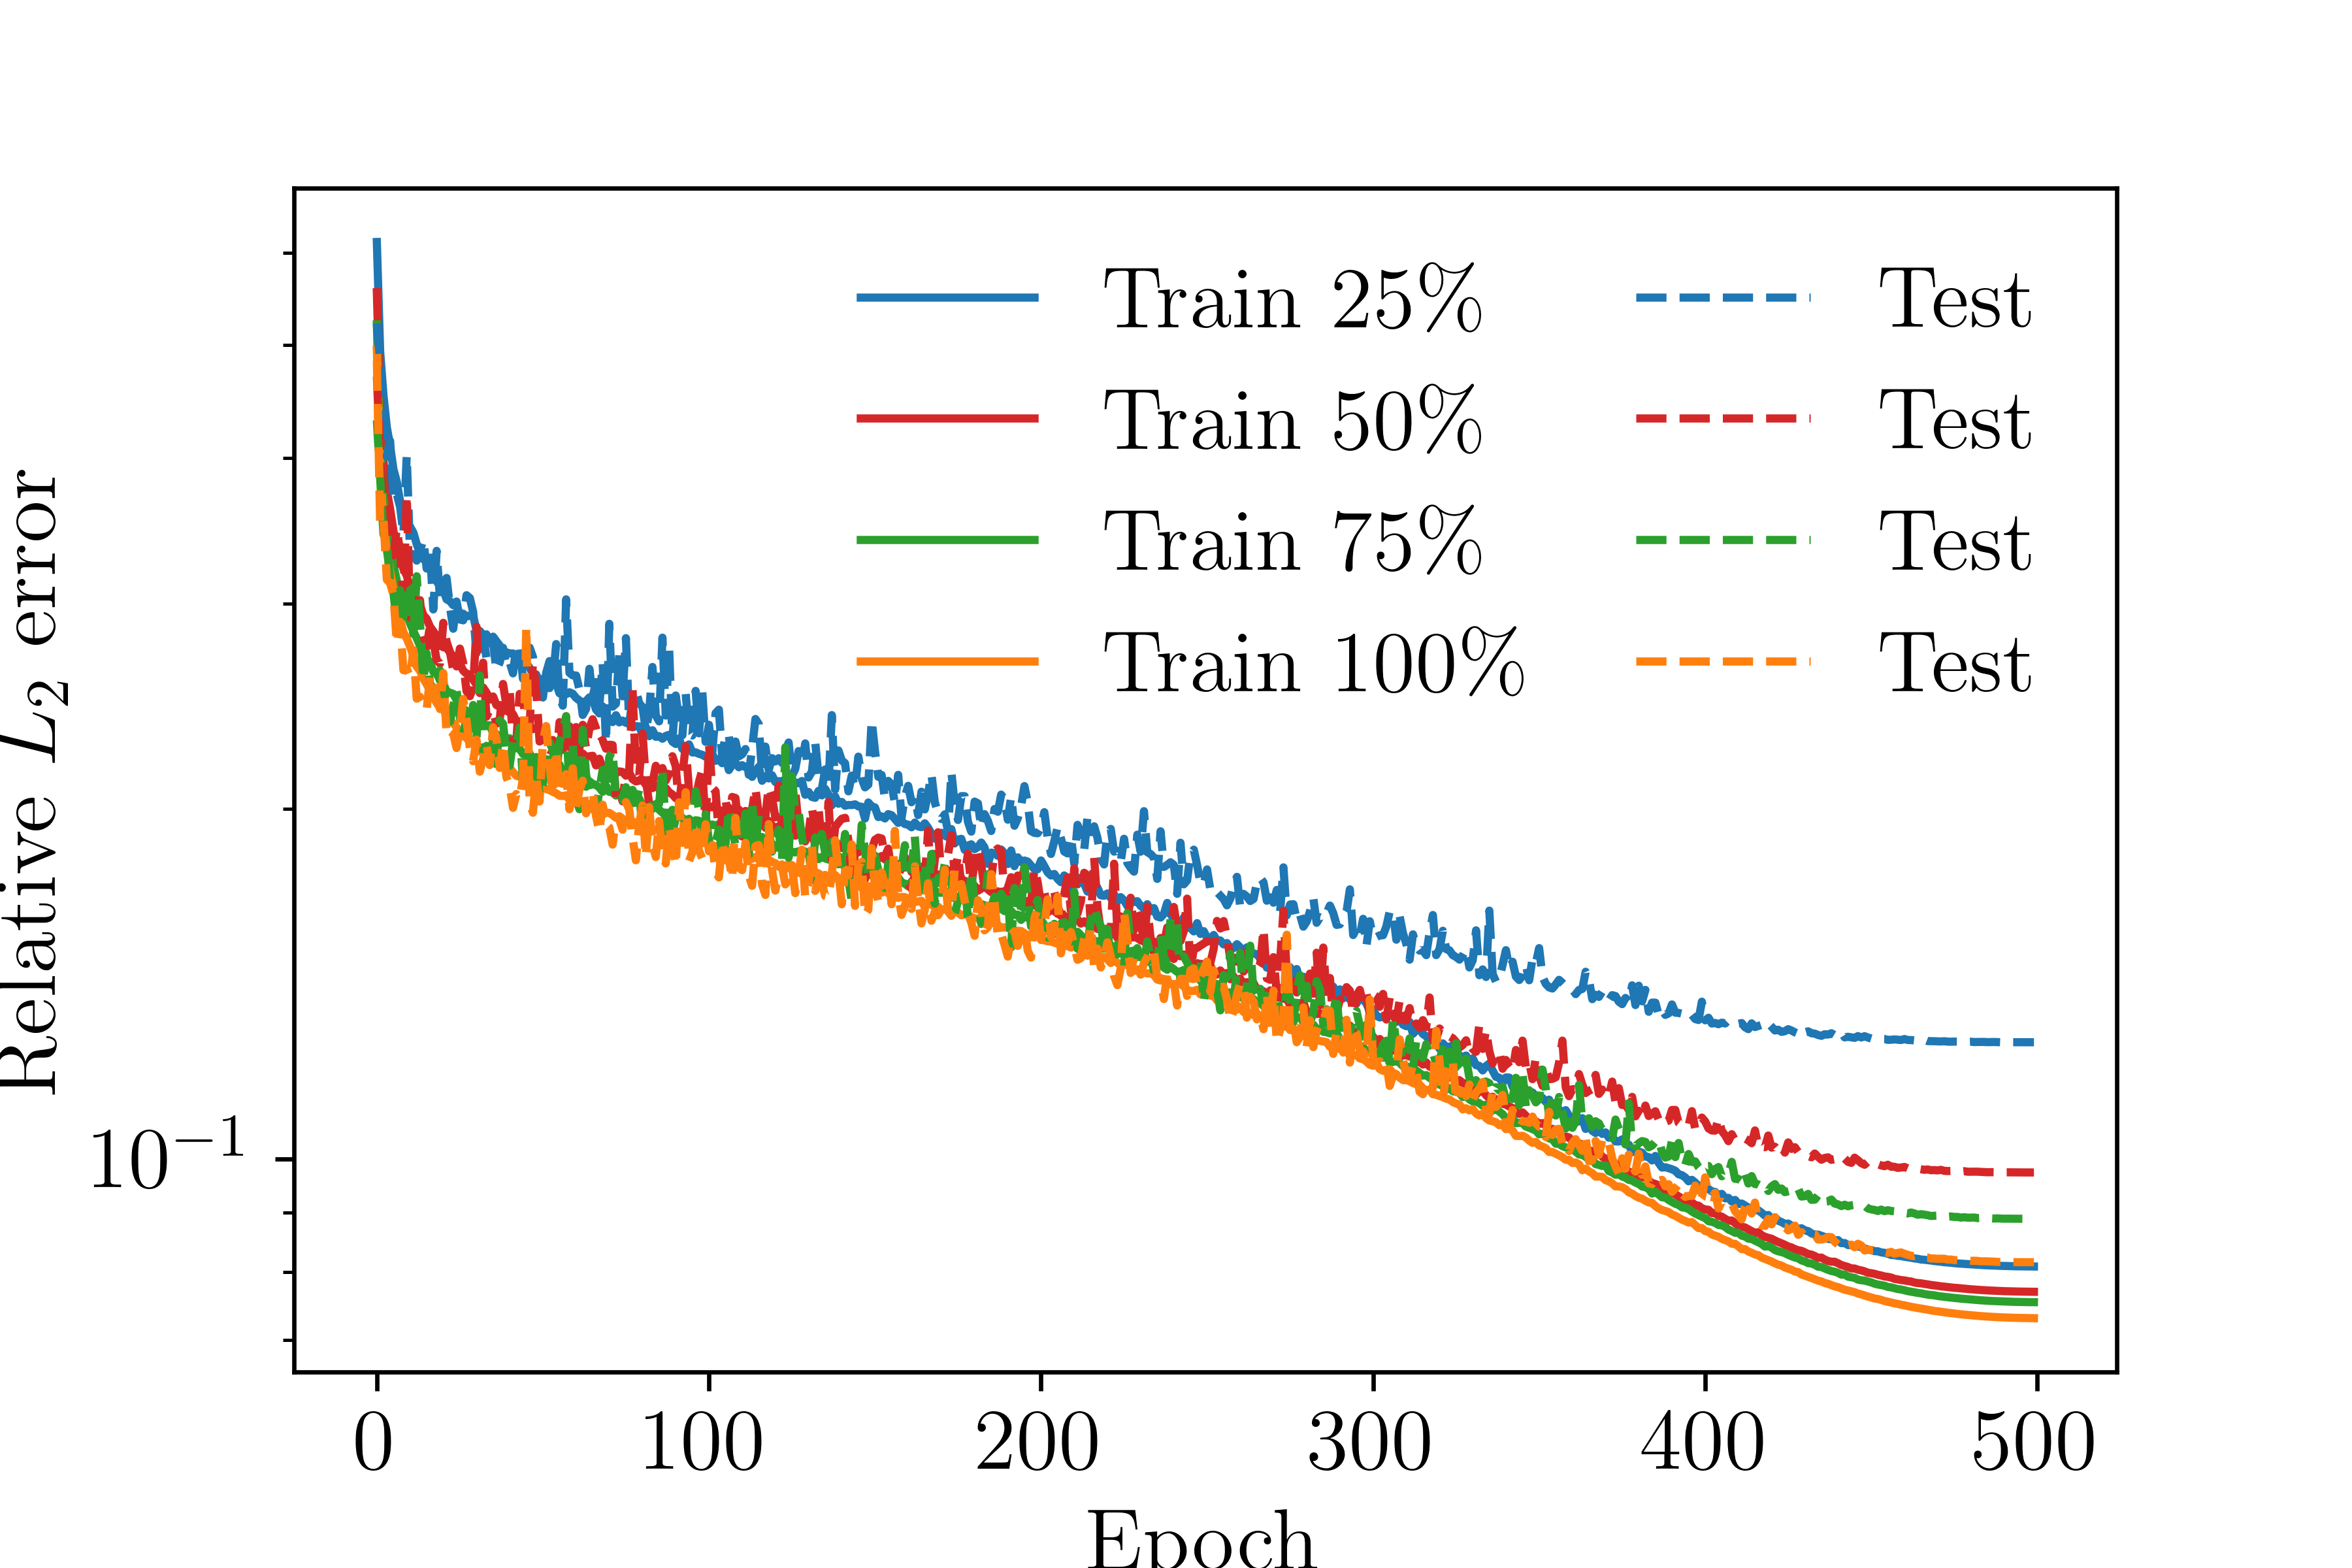
\includegraphics[width=0.7\linewidth]{loss_numdata_2.png}
    \DIFaddendFL \caption{\DIFdelbeginFL %DIFDELCMD < \label{fig:heatmap}%%%
\DIFdelFL{Heat map showing the relative \(L_2\) error of 100 }\DIFdelendFL \DIFaddbeginFL \label{fig:loss_numdata} \DIFaddFL{Training and }\DIFaddendFL testing \DIFdelbeginFL \DIFdelFL{sets with inputs }\DIFdelendFL \DIFaddbeginFL \DIFaddFL{losses for different numbers }\DIFaddendFL of \DIFdelbeginFL \DIFdelFL{fractal stress distribution at \(D=1.6\) }\DIFdelendFL \DIFaddbeginFL \DIFaddFL{training realizations: 25\%, 50\%, 75\%, }\DIFaddendFL and \DIFdelbeginFL \DIFdelFL{frictional parameters \(\Delta a_{0}=0.012\) and \(a_{0}=0.006\). The number }\DIFdelendFL \DIFaddbeginFL \DIFaddFL{100\% }\DIFaddendFL of \DIFdelbeginFL \DIFdelFL{modes and the widths of \(P\) and \(Q\) are shown on the vertical and horizontal axes}\DIFdelendFL \DIFaddbeginFL \DIFaddFL{7}\DIFaddendFL ,\DIFdelbeginFL \DIFdelFL{respectively}\DIFdelendFL \DIFaddbeginFL \DIFaddFL{380 sets. Solid lines show training losses}\DIFaddendFL , \DIFdelbeginFL \DIFdelFL{with (a) a learning rate of 0.0005 }\DIFdelendFL and \DIFdelbeginFL \DIFdelFL{(b) a learning rate of 0.001}\DIFdelendFL \DIFaddbeginFL \DIFaddFL{dashed lines show testing losses}\DIFaddendFL .}
\end{figure}


\DIFdelbegin %DIFDELCMD < \begin{figure}
%DIFDELCMD < \centering
%DIFDELCMD < \includegraphics[width=1.0\linewidth]{tuninig_set6_R2.png}
%DIFDELCMD < %%%
%DIFDELCMD < \caption{%
{%DIFAUXCMD
%DIFDELCMD < \label{fig:tuning_set6} %%%
\DIFdelFL{Results from FNO-1D (dashed red) are compared with those from the specialized FNO (dashed orange), which is trained on 900 separate sets of fractal stress distributions with \(D=1.6\) and frictional parameters \(a\) and \(b\) (with \(\Delta a_{0}=0.012\) and \(a_{0}=0.006\); dashed orange) and with the ground truth (solid blue). (a) and (b) show the inputs, including the initial shear stress and frictional parameters, while (c) - (f) are the outputs, consisting of predicted slip rate snapshots at selected discrete time steps.
}}
%DIFAUXCMD
%DIFDELCMD < \end{figure}
%DIFDELCMD < %%%
\DIFdelend %DIF >  To improve accuracy, we propose training exclusively on a specific dataset with a chosen fractal dimension and frictional parameters. Here, we select a dataset with \(D=1.6\), \(\Delta a_0 = 0.012\), and \(a_0 = 0.006\) resulting in a training set of 900 realizations and a testing set of 100 realizations. We primarily tune the number of Fourier modes, the width of the lifting and projection layers, and the learning rate. The relative \(L_2\) error for the testing set is shown in Figure \ref{fig:heatmap}. The number of modes is increased to 16, 32, 64, 128. We observe a decrease in error when increasing the depth of the fully connected layers \(P\) and \(Q\).  The most influential hyperparameter is the width when using a learning rate of 0.001. It is evident that the relative \(L_2\) error decreases as the widths of \(P\) and \(Q\) increase, as indicated by the blue gradient on the right side of the heat map. Other hyperparameters, including the number of Fourier layers, the number of retained Fourier modes, and the learning rate, do not exhibit a clear pattern, and the error fluctuates. 

%DIF >  After hyperparameter tuning, the revised model demonstrates enhanced predictive accuracy, with the predicted slip rates illustrated in Figure \ref{fig:tuning_set6}. In the zoomed inset of panel (f), the specialized FNO captures some high-frequency components better than the original FNO at \( x \approx -10 \) and \(x \approx 10\) km. This improvement paves the way for further increasing the complexity of the FNO in future work.
\DIFaddbegin 

%DIF >  \begin{figure}
%DIF >      \centering
%DIF >      \includegraphics[width=0.8\linewidth]{figures/V1/heatmap.png}
%DIF >      \caption{\label{fig:heatmap}Heat map showing the relative \(L_2\) error of 100 testing sets with inputs of fractal stress distribution at \(D=1.6\) and frictional parameters \(\Delta a_{0}=0.012\) and \(a_{0}=0.006\). The number of modes and the widths of \(P\) and \(Q\) are shown on the vertical and horizontal axes, respectively, with (a) a learning rate of 0.0005 and (b) a learning rate of 0.001.}
%DIF >  \end{figure}

%DIF >  \begin{figure}
%DIF >  \centering
%DIF >  \includegraphics[width=1.0\linewidth]{figures/V1/tuninig_set6_R2.png}
%DIF >  \caption{\label{fig:tuning_set6} Results from FNO-1D (dashed red) are compared with those from the specialized FNO (dashed orange), which is trained on 900 separate sets of fractal stress distributions with \(D=1.6\) and frictional parameters \(a\) and \(b\) (with \(\Delta a_{0}=0.012\) and \(a_{0}=0.006\); dashed orange) and with the ground truth (solid blue). (a) and (b) show the inputs, including the initial shear stress and frictional parameters, while (c) - (f) are the outputs, consisting of predicted slip rate snapshots at selected discrete time steps.
%DIF >  }
%DIF >  \end{figure}


\DIFaddend For the 3D dynamic rupture dataset, we primarily tune the model while keeping the number of Fourier layers fixed at four, based on insights from the 2D dynamic rupture dataset. The number of retained Fourier modes is initially selected as 16, 32, and 64, while the depth of \(P\) and \(Q\) is chosen from 32, 64, and 128. We consider learning rates of 0.001 and 0.0005. The results of the tuning process are presented in Table \ref{tab:3D_hyperparam}. The optimal model is selected with four Fourier layers, 32 Fourier modes, 128 neurons in \(P\) and \(Q\), and a learning rate of 0.001.


\begin{table}[ht!]
\caption{Relative \( L_2 \) errors for different hyperparameter configurations, including the number of Fourier layers, modes, learning rate, and the widths of \( P \) and \( Q \), tested on data from a 3D simulation of dynamic rupture.}
    \centering
    \begin{tabular}{ccccc}
        \toprule
        \textbf{Learning Rate} & \textbf{Modes} & \multicolumn{3}{c}{\textbf{Width of \(P\) and \(Q\)}} \\
        \cmidrule(lr){3-5}
        & & 32 & 64 & 128 \\
        \midrule
        % 4 Layers Results
        0.001  & 16  & 0.127383 & 0.115418 & 0.113272  \\
               & 32  & 0.108283 & 0.105937 & \textbf{0.080965}  \\
               & 64  & 0.102793 & 0.126559 & 0.114296  \\
        0.0005 & 16  & 0.123509 & 0.093694  & 0.107529  \\
               & 32  & 0.101131 & 0.096700  & 0.083106  \\
               & 64  & 0.096357 & 0.106043 & 0.091511 \\
        \bottomrule
    \end{tabular}
    \label{tab:3D_hyperparam}
\end{table}

\DIFaddbegin \section{\DIFadd{Quantitative Analysis of Prediction Error}}
\label{sec:appendix_c}

\DIFadd{As an additional validation metric, we compare the FNO predictions against the ground truth using the \(Q\) metric, which is specifically designed for time-series comparisons in dynamic rupture simulations~\mbox{%DIFAUXCMD
\cite{barall2015metrics}}\hskip0pt%DIFAUXCMD
. The \(Q\) metric is defined as
}\begin{equation}
    \DIFadd{Q(t_s) = 
    \frac{\lVert f(t) - g(t - t_s) \rVert_2}{\lVert f(t) \rVert_2 + \lVert g(t - t_s) \rVert_2},
    \label{Q}
}\end{equation}
\DIFadd{where \(f(t)\) denotes the vector of slip rate predictions from the FNO model, \(g(t)\) represents the corresponding ground truth values, and \(t_s\) is a temporal shift applied to align the signals. The optimal time shift is obtained as
}\begin{equation}
    \DIFadd{t_s^\star \in \arg\min_{t_s} Q(t_s).
    \label{t_s}
}\end{equation}
\DIFadd{A smaller \(Q\) value indicates closer agreement between prediction and ground truth.
}

\DIFadd{For illustration, we select three representative cases from the 3D dynamic rupture dataset, corresponding to relative \(L_2\) errors equal to the median, median\,+\,2MAD, and median\,+\,4MAD. For each case, we compute \(Q\) and report the associated optimal shift \(t_s^\star\).
}

\DIFadd{Figures~\ref{fig:app_med}--\ref{fig:app_med_4mad} present the rupture front evolution and slip rate histories for these cases. The computed \(Q\) values are 12.94\%, 20.6\%, and 39.6\%, with corresponding optimal time shifts \(t_s^\star\) of 0.005\,s, 0.004\,s, and 0.025\,s, respectively. Figure~\ref{fig:rel_err_peak} shows the relative error of the peak $V_{zx}$ as a function of time step for the case with relative $L_{2}$ error closes to the median. The error increases after time step~40, which marks the stage when the rupture arrives at the VS boundaries. This introduces higher-frequency components into the slip rate field that are more challenging to capture. Additional contributing factors include the limited availability of training samples, particularly for cases where the rupture reaches the boundaries, the restriction imposed by the chosen number of modes in the FNO, and the inherent spectral bias of neural operators.
}



\begin{figure}
    \centering
    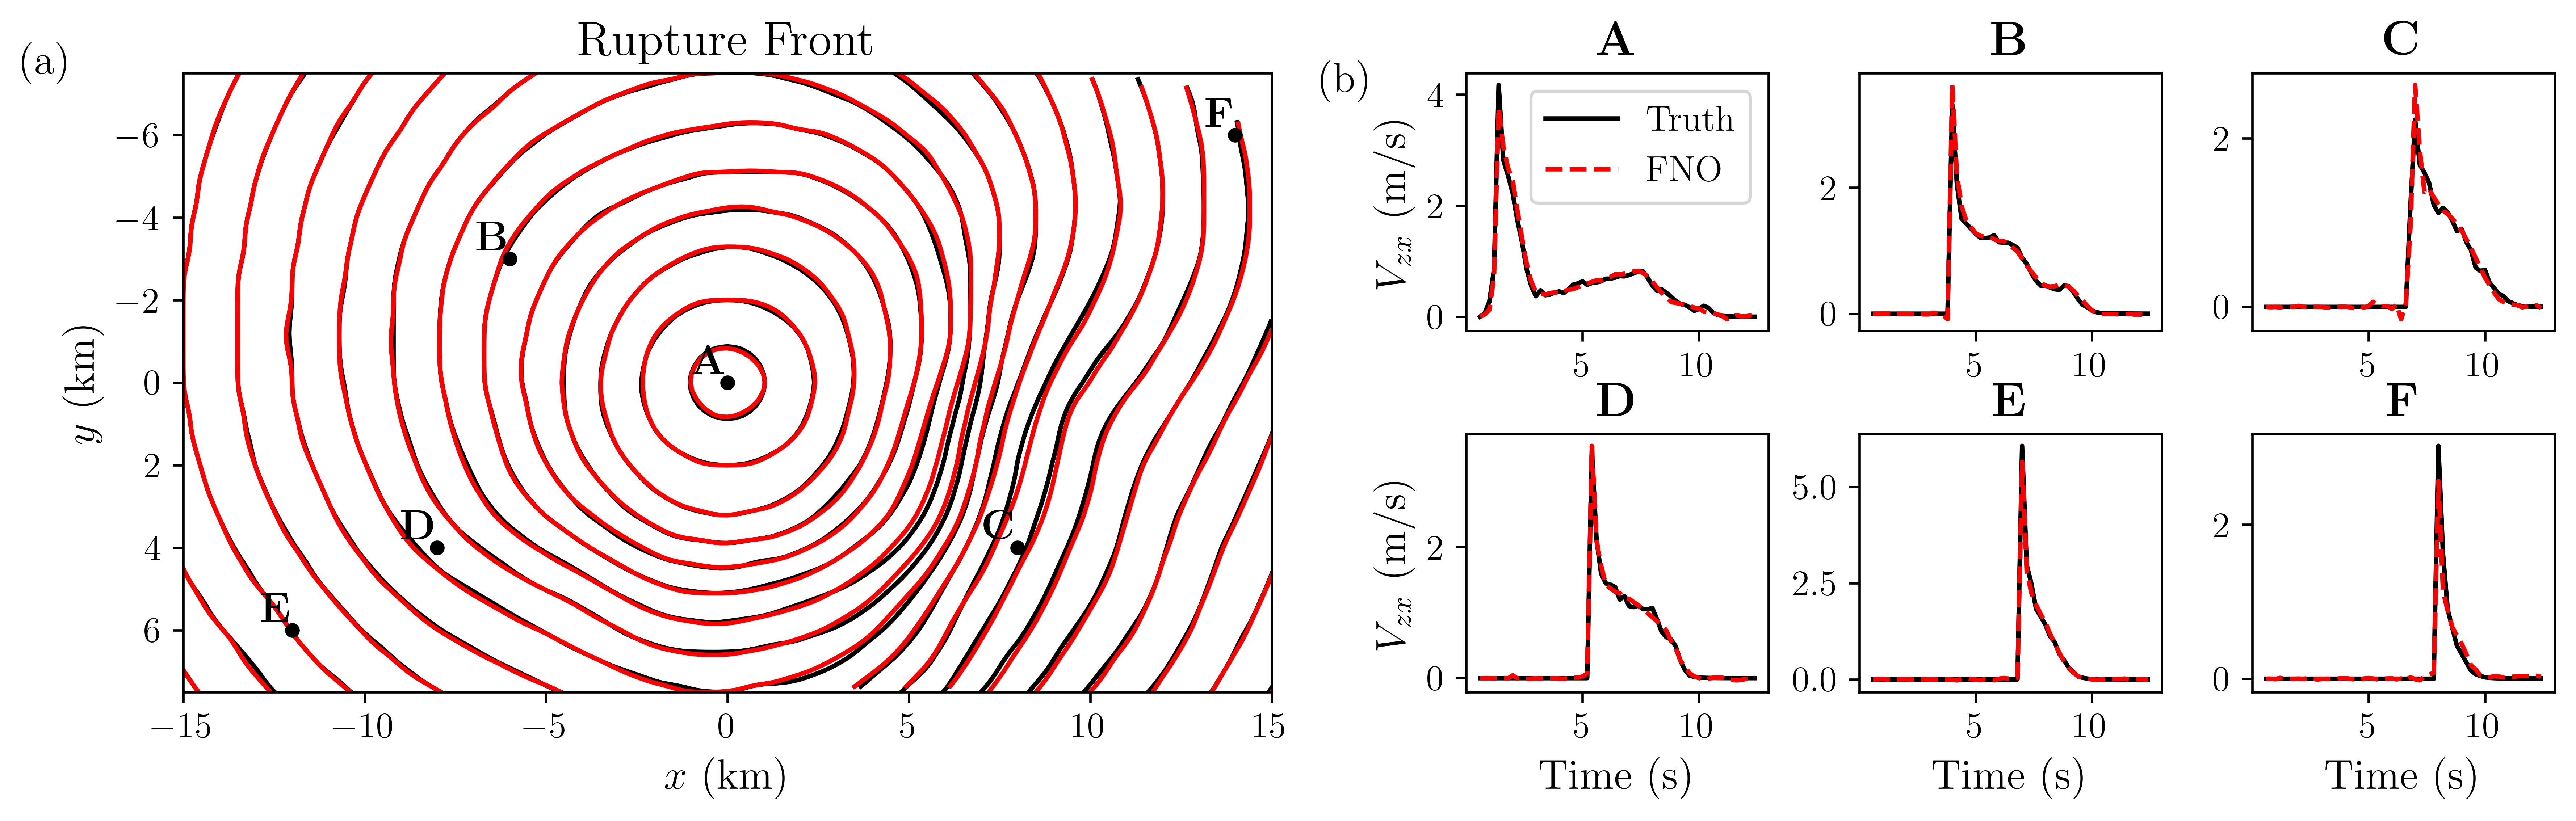
\includegraphics[width=1.0\linewidth]{app_med.png}
    \caption{\label{fig:app_med} \DIFaddFL{Results of FNO-2D on the testing dataset for a 3D dynamic rupture case with a relative \(L_2\) error of 0.130 (median) and an NRMSE of 0.00354. The inputs include the initial fractal shear stress (\(D = 1.5\)), the initial \(V_{zx}\) field (\(V_\text{th} = 10^{-3}\,\mathrm{m/s}\)), a nucleation perturbation, and frictional parameters \(a\) (\(a_0 = 0.008\), \(\Delta a_0 = 0.008\)) and \(b = 0.012\). (a) Rupture front contours at 0.5\,s intervals. (b) Time histories of slip rate at selected spatial locations.}}
\end{figure}

\begin{figure}
    \centering
    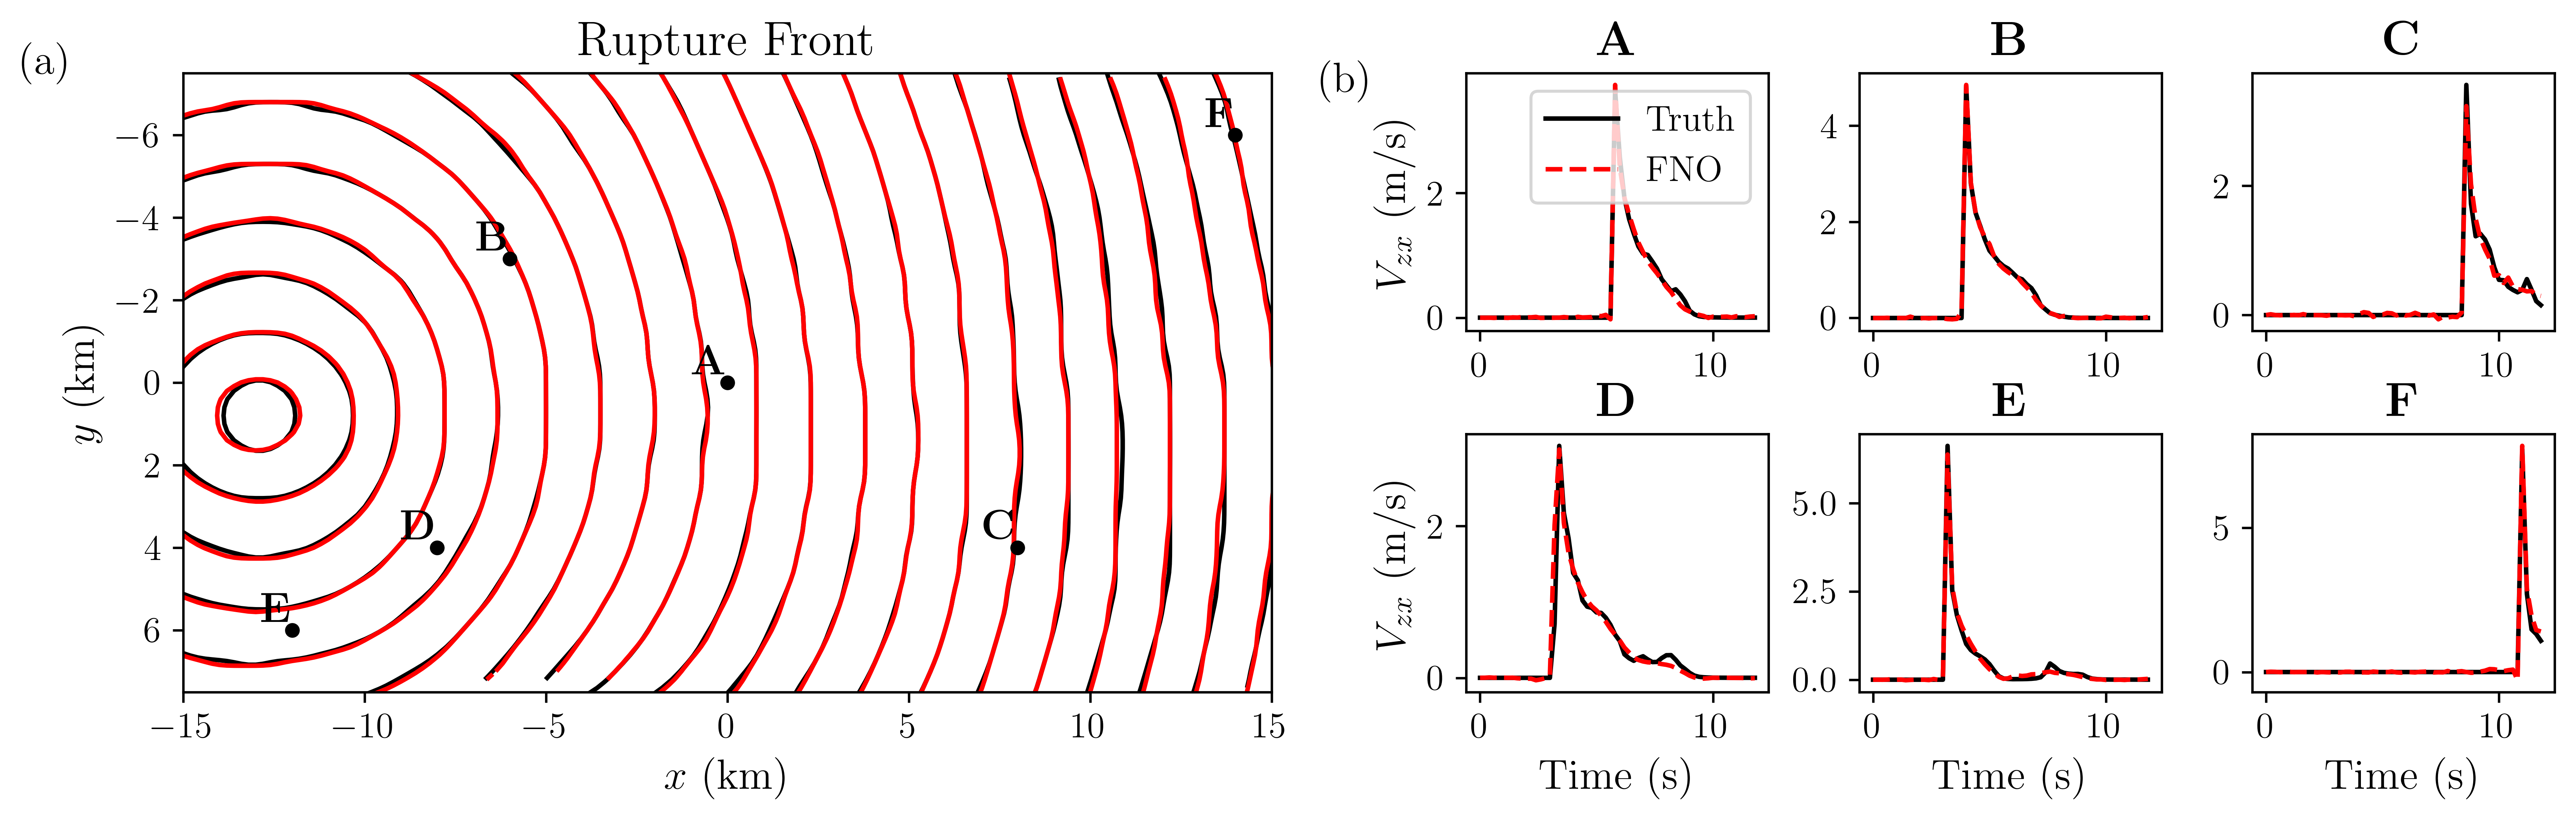
\includegraphics[width=1.0\linewidth]{app_med_2mad.png}
    \caption{\label{fig:app_med_2mad} \DIFaddFL{Results of FNO-2D on the testing dataset for a 3D dynamic rupture case with a relative \(L_2\) error of 0.207 (median\,+\,2MAD) and an NRMSE of 0.00531. The inputs include the initial fractal shear stress (\(D = 1.2\)), the initial \(V_{zx}\) field (\(V_\text{th} = 10^{-3}\,\mathrm{m/s}\)), a nucleation perturbation, and frictional parameters \(a\) (\(a_0 = 0.008\), \(\Delta a_0 = 0.008\)) and \(b = 0.012\). (a) Rupture front contours at 0.5\,s intervals. (b) Time histories of slip rate at selected spatial locations.}}
\end{figure}

\begin{figure}
    \centering
    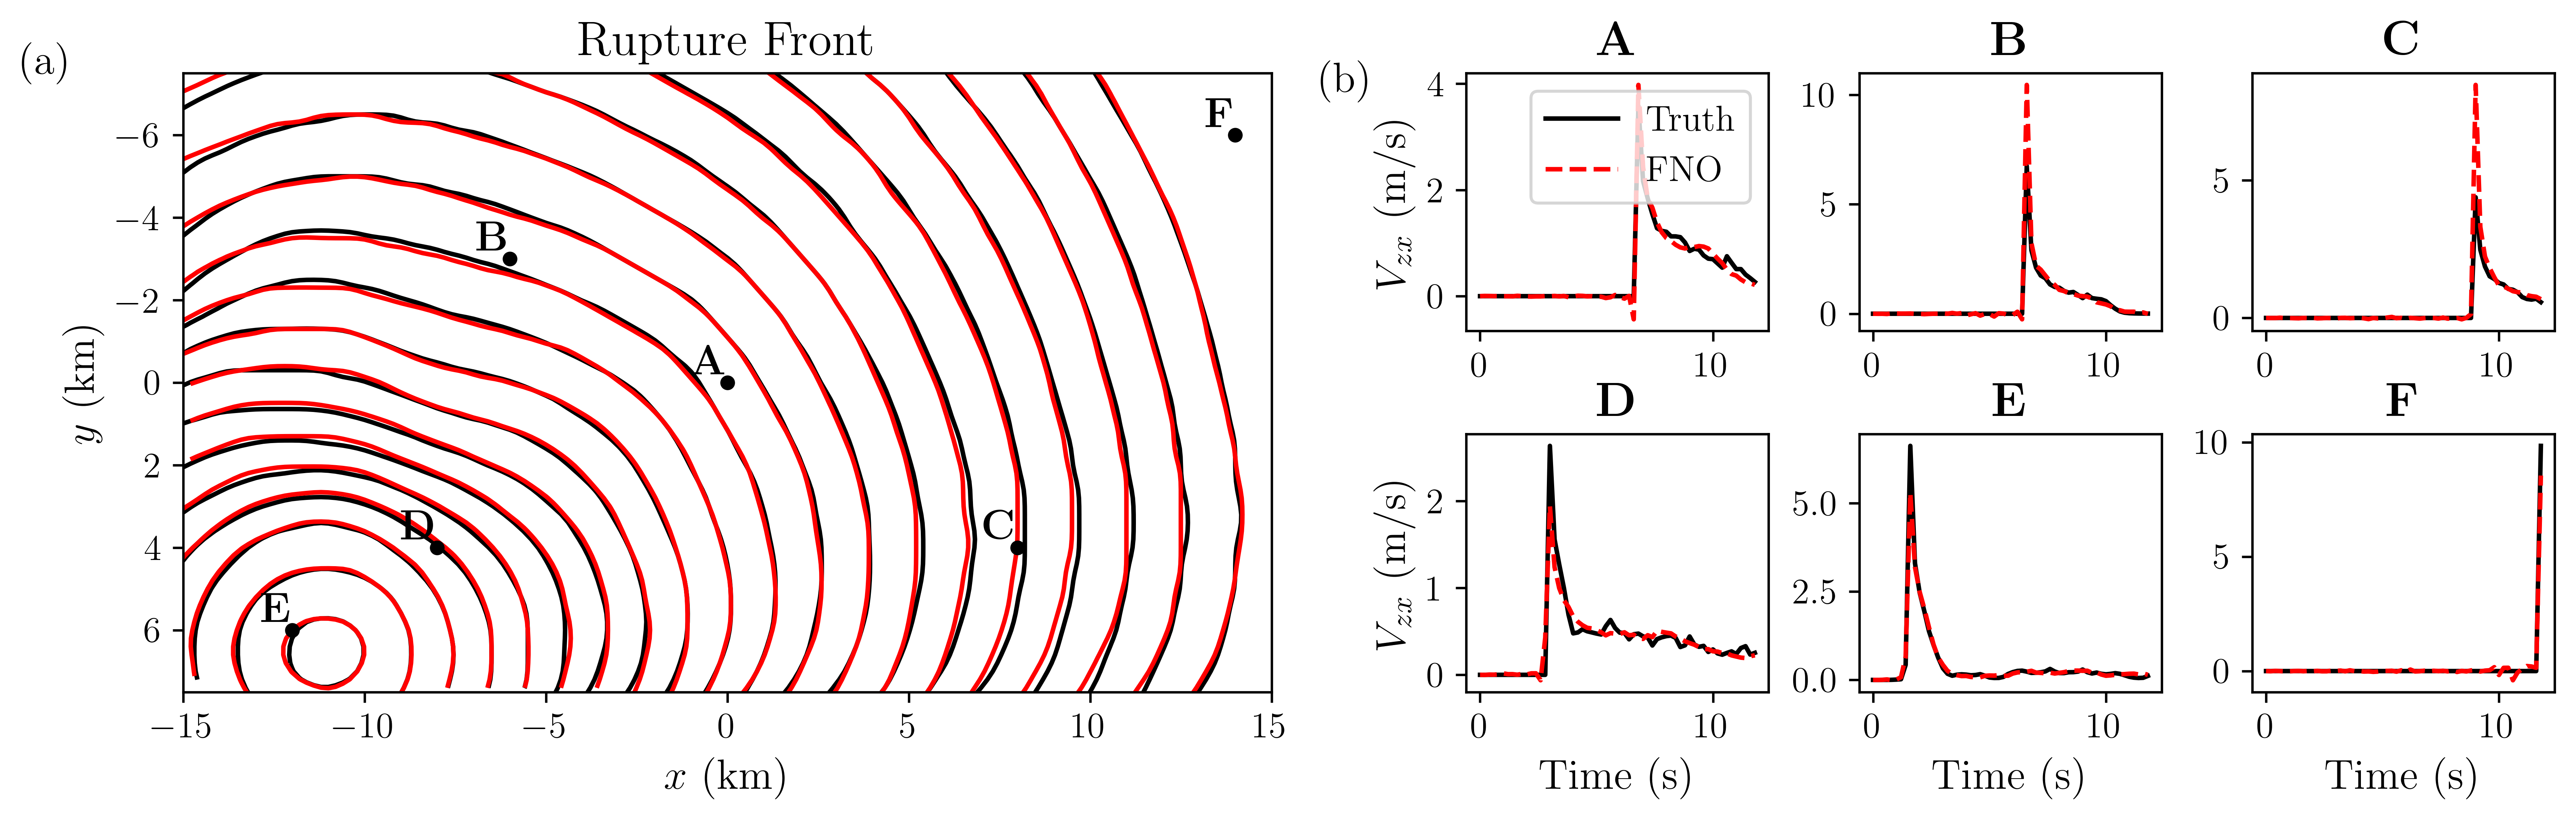
\includegraphics[width=1.0\linewidth]{app_med_4mad.png}
    \caption{\label{fig:app_med_4mad} \DIFaddFL{Results of FNO-2D on the testing dataset for a 3D dynamic rupture case with a relative \(L_2\) error of 0.408 (median\,+\,4MAD) and an NRMSE of 0.0108. The inputs include the initial fractal shear stress (\(D = 1.6\)), the initial \(V_{zx}\) field (\(V_\text{th} = 0\,\mathrm{m/s}\)), a nucleation perturbation, and frictional parameters \(a\) (\(a_0 = 0.008\), \(\Delta a_0 = 0.008\)) and \(b = 0.012\). (a) Rupture front contours at 0.5\,s intervals. (b) Time histories of slip rate at selected spatial locations.}}
\end{figure}

\begin{figure}
    \centering
    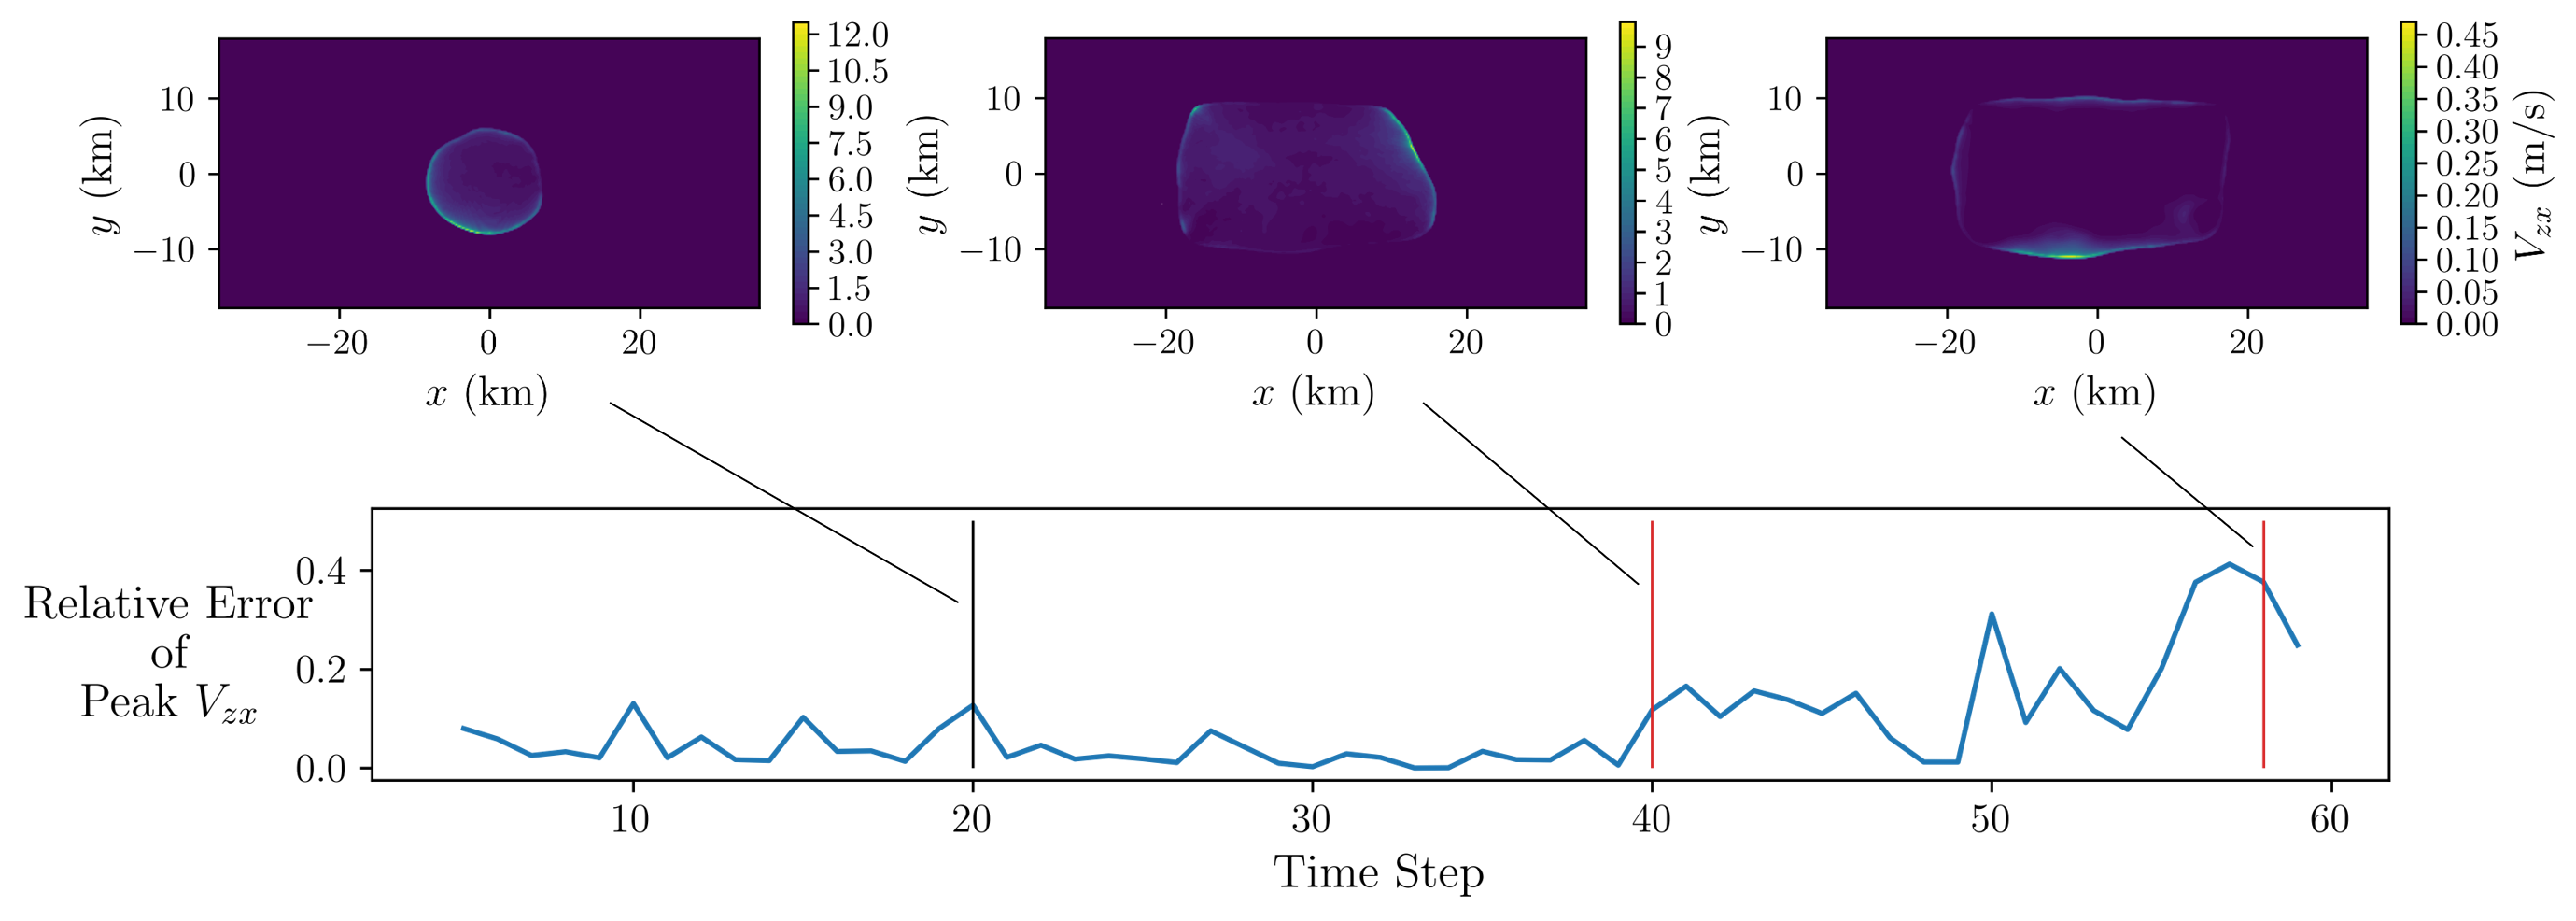
\includegraphics[width=0.9\linewidth]{error_time_2.png}
    \caption{\label{fig:rel_err_peak} \DIFaddFL{Top: Contours of the ground-truth slip rate $V_{zx}$ at time steps 20, 40, and 58, illustrating rupture propagation and the stages when rupture reaches the fault boundaries. Bottom: Temporal evolution of the relative error in the peak slip rate, with vertical lines marking the reference time steps (20, 40, and 58). The last two vertical lines (in red) indicate when the rupture front reaches the boundaries, leading to higher error due to the emergence of high-frequency components.}}
\end{figure}



\DIFaddend \section*{Open Research}
All data used in the analysis are available online at \citeA{tainpakdipat2025}. The FNO software used to conduct the numerical experiments will be made available upon acceptance.




\acknowledgments
The study was supported by the National Science Foundation (CAREER award No. 1753249 and OAC-2311207) and the Southern/Statewide California Earthquake Center (based on NSF Cooperative Agreement EAR-1600087 and USGS Cooperative Agreement G17AC00047). We also acknowledge funding provided by DOE EERE Geothermal Technologies Office to Utah FORGE and the University of Utah under Project DE-EE0007080 Enhanced Geothermal System Concept Testing and Development at the Milford City, Utah Frontier Observatory for Research in Geothermal Energy (Utah FORGE) site. \DIFaddbegin \DIFadd{This work used Delta at the National Center for Supercomputing Applications (NCSA) through allocation EES230038 from the Advanced Cyberinfrastructure Coordination Ecosystem: Services \& Support (ACCESS) program, which is supported by U.S. National Science Foundation grants \#2138259, \#2138286, \#2138307, \#2137603, and \#2138296.
}\DIFaddend 


\bibliography{cas-refs}

\end{document}



More Information and Advice:

%%%%%%%%%%%%%%%%%%%%%%%%%%%%%%%%%%%%%%%%%%%%%%%
%
%  SECTION HEADS
%
%%%%%%%%%%%%%%%%%%%%%%%%%%%%%%%%%%%%%%%%%%%%%%%

% Capitalize the first letter of each word (except for
% prepositions, conjunctions, and articles that are
% three or fewer letters).

% AGU follows standard outline style; therefore, there cannot be a section 1 without
% a section 2, or a section 2.3.1 without a section 2.3.2.
% Please make sure your section numbers are balanced.
% ---------------
% Level 1 head
%
% Use the \section{} command to identify level 1 heads;
% type the appropriate head wording between the curly
% brackets, as shown below.
%
%An example:
%\section{Level 1 Head: Introduction}
%
% ---------------
% Level 2 head
%
% Use the \subsection{} command to identify level 2 heads.
%An example:
%\subsection{Level 2 Head}
%
% ---------------
% Level 3 head
%
% Use the \subsubsection{} command to identify level 3 heads
%An example:
%\subsubsection{Level 3 Head}
%
%---------------
% Level 4 head
%
% Use the \subsubsubsection{} command to identify level 3 heads
% An example:
%\subsubsubsection{Level 4 Head} An example.
%
%%%%%%%%%%%%%%%%%%%%%%%%%%%%%%%%%%%%%%%%%%%%%%%
%
%  IN-TEXT LISTS
%
%%%%%%%%%%%%%%%%%%%%%%%%%%%%%%%%%%%%%%%%%%%%%%%
%
% Do not use bulleted lists; enumerated lists are okay.
% \begin{enumerate}
% \item
% \item
% \item
% \end{enumerate}
%
%%%%%%%%%%%%%%%%%%%%%%%%%%%%%%%%%%%%%%%%%%%%%%%
%
%  EQUATIONS
%
%%%%%%%%%%%%%%%%%%%%%%%%%%%%%%%%%%%%%%%%%%%%%%%

% Single-line equations are centered.
% Equation arrays will appear left-aligned.

Math coded inside display math mode \[ ...\]
 will not be numbered, e.g.,:
 \[ x^2=y^2 + z^2\]

 Math coded inside \begin{equation} and \end{equation} will
 be automatically numbered, e.g.,:
 \begin{equation}
 x^2=y^2 + z^2
 \end{equation}


% To create multiline equations, use the
% \begin{eqnarray} and \end{eqnarray} environment
% as demonstrated below.
\begin{eqnarray}
  x_{1} & = & (x - x_{0}) \cos \Theta \nonumber \\
        && + (y - y_{0}) \sin \Theta  \nonumber \\
  y_{1} & = & -(x - x_{0}) \sin \Theta \nonumber \\
        && + (y - y_{0}) \cos \Theta.
\end{eqnarray}

%If you don't want an equation number, use the star form:
%\begin{eqnarray*}...\end{eqnarray*}

% Break each line at a sign of operation
% (+, -, etc.) if possible, with the sign of operation
% on the new line.

% Indent second and subsequent lines to align with
% the first character following the equal sign on the
% first line.

% Use an \hspace{} command to insert horizontal space
% into your equation if necessary. Place an appropriate
% unit of measure between the curly braces, e.g.
% \hspace{1in}; you may have to experiment to achieve
% the correct amount of space.


%%%%%%%%%%%%%%%%%%%%%%%%%%%%%%%%%%%%%%%%%%%%%%%
%
%  EQUATION NUMBERING: COUNTER
%
%%%%%%%%%%%%%%%%%%%%%%%%%%%%%%%%%%%%%%%%%%%%%%%

% You may change equation numbering by resetting
% the equation counter or by explicitly numbering
% an equation.

% To explicitly number an equation, type \eqnum{}
% (with the desired number between the brackets)
% after the \begin{equation} or \begin{eqnarray}
% command.  The \eqnum{} command will affect only
% the equation it appears with; LaTeX will number
% any equations appearing later in the manuscript
% according to the equation counter.
%

% If you have a multiline equation that needs only
% one equation number, use a \nonumber command in
% front of the double backslashes (\\) as shown in
% the multiline equation above.

% If you are using line numbers, remember to surround
% equations with \begin{linenomath*}...\end{linenomath*}

%  To add line numbers to lines in equations:
%  \begin{linenomath*}
%  \begin{equation}
%  \end{equation}
%  \end{linenomath*}
